% Documents setup
\documentclass[11pt]{book}

% fix for pandoc 1.14
\providecommand{\tightlist}{%
  \setlength{\itemsep}{0pt}\setlength{\parskip}{0pt}}

\usepackage{tabu} % https://tex.stackexchange.com/questions/50332/vertical-spacing-of-a-table-cell

% Location of the csas-style repository: adjust path as needed
\newcommand{\locRepo}{csas-style}

% Use the style file in the csas-style repository (res-doc.sty)
\usepackage{\locRepo/res-doc}

% header-includes from R markdown entry


% Headers and footers
\lhead{Draft working paper --- Do not cite or circulate}
% \lhead{}
\rhead{}
% \rfoot{DRAFT - DO NOT CITE}

%%%% Commands for title page etc %%%%%

% Publication year
\newcommand{\rdYear}{2025}

% Publication month
\newcommand{\rdMonth}{Month}

% Report number
\newcommand{\rdNumber}{nnn}

% Region
\newcommand{\rdRegion}{Pacific Region}

% Title
\newcommand{\rdTitle}{Stock status and biological and fishery consequences of alternative harvest and rebuilding actions for Yukon River Chinook salmon (\emph{Oncorhynchus tshawytscha})}

\newcommand{\rdISBN}{978-0-660-38322-4}
\newcommand{\rdCatNo}{Fs70-6/2021-012E-PDF}

% Author names separated by commas and ', and' for the last author in the format 'M.H. Grinnell' (use \textsuperscript{n} for addresses)
\newcommand{\rdAuth}{Brendan M. Connors\textsuperscript{1}, Adam O'Dell\textsuperscript{2}, Hannah Hunter\textsuperscript{3}, Dylan Glaser\textsuperscript{4}, Jessica Gill\textsuperscript{3}, Steven Rossi\textsuperscript{5}, Carolyn Churchland\textsuperscript{3}, and Cheyenne Bradley\textsuperscript{2}}

% Author names reversed separated by commas in the format 'Grinnell, M.H.'
\newcommand{\rdAuthRev}{Connors, B.M., O'Dell, A., Hunter, H., Glaser, D., Gill, J., Rossi, S., Churchland, C., and Bradley, C.}

% Author addresses (use \textsuperscript{n})
\newcommand{\rdAuthAddy}{\textsuperscript{1}Institute of Ocean Sciences\\
Fisheries and Oceans Canada, 9860 W. Saanich Road\\
Sidney, British Columbia, V8L 5T5, Canada\\
\smallskip \textsuperscript{2}Yukon Rivers and Transboundary Area~ Fisheries and Oceans Canada, 419 Range Road\\
Whitehorse, Yukon Territory, Y0A 0A2, Canada~ \smallskip \textsuperscript{3}Regional Headquarters (Pacific)\\
Fisheries and Oceans Canada, 200-401 Burrard Street\\
Vancouver, British Columbia, V6C 3S4, Canada\\
\smallskip \textsuperscript{4}Pacific Biological Station\\
Fisheries and Oceans Canada, 3190 Hammond Bay Road\\
Nanaimo, British Columbia, V9T 6N7, Canada\\
\smallskip \textsuperscript{5}LGL Limited~ 9768 Second Street\\
Sidney, British Columbia, V8L 3Y8, Canada~}

\newcommand{\citationOtherLanguage}{Last, F.M. et Smith, A.B. Title Here (\emph{Latin Species Name}). DFO Secr. can. des avis sci. du MPO. Doc. de rech 2019/nnn. iv + 13 p.}

% Name of file with abstract and resume (see \abstract in inst/csas-style/res-doc.sty)
\newcommand{\rdAbstract}{\abstract{Here is the abstract text. Lorem ipsum dolor sit amet, consectetur adipisicing elit, sed do eiusmod tempor incididunt ut labore et dolore magna aliqua. Ut enim ad minim veniam, quis nostrud exercitation ullamco laboris nisi ut aliquip ex ea commodo consequat. Duis aute irure dolor in reprehenderit in voluptate velit esse cillum dolore eu fugiat nulla pariatur. Excepteur sint occaecat cupidatat non proident, sunt in culpa qui officia deserunt mollit anim id est laborum. \vspace{1.5mm} \break Start new paragraphs after a blank line and with 2 spaces indent. Lorem ipsum dolor sit amet, consectetur adipisicing elit, sed do eiusmod tempor incididunt ut labore et dolore magna aliqua. Ut enim ad minim veniam, quis nostrud exercitation ullamco laboris nisi ut aliquip ex ea commodo consequat. Duis aute irure dolor in reprehenderit in voluptate velit esse cillum dolore eu fugiat nulla pariatur. Excepteur sint occaecat cupidatat non proident, sunt in culpa qui officia deserunt mollit anim id est laborum.}}

%%%% End of title page commands %%%%%

% \pdfcompresslevel=5 % faster PNGs

\setcounter{section}{0}

\bibliographystyle{csas-style/res-doc}

\usepackage{amsmath}
\usepackage{bm}

% commands and environments needed by pandoc snippets
% extracted from the output of `pandoc -s`
%% Make R markdown code chunks work
\usepackage{array}
\usepackage{amssymb,amsmath}
\usepackage{color}
\usepackage{fancyvrb}

% From default template:
\newcommand{\VerbBar}{|}
\newcommand{\VERB}{\Verb[commandchars=\\\{\}]}
\DefineVerbatimEnvironment{Highlighting}{Verbatim}{commandchars=\\\{\},formatcom=\color[rgb]{0.00,0.00,0.00}}
\usepackage{framed}
\definecolor{shadecolor}{RGB}{248,248,248}
\newenvironment{Shaded}{\begin{snugshade}}{\end{snugshade}}
\newcommand{\AlertTok}[1]{\textcolor[rgb]{0.94,0.16,0.16}{#1}}
\newcommand{\AnnotationTok}[1]{\textcolor[rgb]{0.56,0.35,0.01}{\textbf{\textit{#1}}}}
\newcommand{\AttributeTok}[1]{\textcolor[rgb]{0.77,0.63,0.00}{#1}}
\newcommand{\BaseNTok}[1]{\textcolor[rgb]{0.00,0.00,0.81}{#1}}
\newcommand{\BuiltInTok}[1]{#1}
\newcommand{\CharTok}[1]{\textcolor[rgb]{0.31,0.60,0.02}{#1}}
\newcommand{\CommentTok}[1]{\textcolor[rgb]{0.56,0.35,0.01}{\textbf{#1}}}
\newcommand{\CommentVarTok}[1]{\textcolor[rgb]{0.56,0.35,0.01}{\textbf{\textit{#1}}}}
\newcommand{\ConstantTok}[1]{\textcolor[rgb]{0.00,0.00,0.00}{#1}}
\newcommand{\ControlFlowTok}[1]{\textcolor[rgb]{0.13,0.29,0.53}{\textit{#1}}}
\newcommand{\DataTypeTok}[1]{\textcolor[rgb]{0.13,0.29,0.53}{#1}}
\newcommand{\DecValTok}[1]{\textcolor[rgb]{0.00,0.00,0.81}{#1}}
\newcommand{\DocumentationTok}[1]{\textcolor[rgb]{0.56,0.35,0.01}{\textbf{\textit{#1}}}}
\newcommand{\ErrorTok}[1]{\textcolor[rgb]{0.64,0.00,0.00}{\textit{#1}}}
\newcommand{\ExtensionTok}[1]{#1}
\newcommand{\FloatTok}[1]{\textcolor[rgb]{0.00,0.00,0.81}{#1}}
\newcommand{\FunctionTok}[1]{\textcolor[rgb]{0.00,0.00,0.00}{#1}}
\newcommand{\ImportTok}[1]{#1}
\newcommand{\InformationTok}[1]{\textcolor[rgb]{0.56,0.35,0.01}{\textbf{\textit{#1}}}}
\newcommand{\KeywordTok}[1]{\textcolor[rgb]{0.13,0.29,0.53}{\textit{#1}}}
\newcommand{\NormalTok}[1]{#1}
\newcommand{\OperatorTok}[1]{\textcolor[rgb]{0.81,0.36,0.00}{\textit{#1}}}
\newcommand{\OtherTok}[1]{\textcolor[rgb]{0.56,0.35,0.01}{#1}}
\newcommand{\PreprocessorTok}[1]{\textcolor[rgb]{0.56,0.35,0.01}{\textbf{#1}}}
\newcommand{\RegionMarkerTok}[1]{#1}
\newcommand{\SpecialCharTok}[1]{\textcolor[rgb]{0.00,0.00,0.00}{#1}}
\newcommand{\SpecialStringTok}[1]{\textcolor[rgb]{0.31,0.60,0.02}{#1}}
\newcommand{\StringTok}[1]{\textcolor[rgb]{0.31,0.60,0.02}{#1}}
\newcommand{\VariableTok}[1]{\textcolor[rgb]{0.00,0.00,0.00}{#1}}
\newcommand{\VerbatimStringTok}[1]{\textcolor[rgb]{0.31,0.60,0.02}{#1}}
\newcommand{\WarningTok}[1]{\textcolor[rgb]{0.56,0.35,0.01}{\textbf{\textit{#1}}}}

\newcommand{\lt}{\ensuremath <}
\newcommand{\gt}{\ensuremath >}

%Defines cslreferences environment
%Required by pandoc 2.8
%Copied from https://github.com/rstudio/rmarkdown/issues/1649
% % \newlength{\cslhangindent}
% \setlength{\cslhangindent}{1.5em}
% \newenvironment{cslreferences}%
%   {}%
%   {\par}
% 
\DeclareGraphicsExtensions{.png,.pdf}
\begin{document}

\frontmatter

\hypertarget{sec:introduction}{%
\section{INTRODUCTION}\label{sec:introduction}}

The Yukon River is the fourth largest, and one of the most isolated, river systems in North America. It drains over 850,000 square kilometers from its headwaters in northern British Columbia through the Yukon Territory and Alaska, U.S. before emptying into the Bering Sea (\protect\hyperlink{ref-brabets2000environmental}{Brabets et al. 2000}). It is also one of the world's largest salmon producing river basins with millions of salmon entering the river in most years (\protect\hyperlink{ref-JTC2025Report}{JTC 2025}). Among these species are Chinook salmon (\emph{Oncorhynchus tshawytscha}) which spawn throughout the basin with nearly half returning to one of the hundreds of Canadian streams to spawn each year (\protect\hyperlink{ref-brown2017}{Brown et al. 2017b}; \protect\hyperlink{ref-JTC2025Report}{JTC 2025}).

Under Canada's Wild Salmon Policy (\protect\hyperlink{ref-WSP2005}{DFO 2005}), Canadian Yukon River Chinook salmon belong to 12 conservation units (CUs) which are genetically and ecologically unique (\protect\hyperlink{ref-holtbyConservationUnitsPacific2007}{Holtby and Ciruna 2007}). These 12 CUs represent 2 stock management units (SMU): Yukon River Chinook salmon and Porcupine Chinook salmon. Canadian-origin Yukon River Chinook salmon are genetically unique within the entire drainage, and sampling in the lower river provides in-season estimates of the Canadian component that enter the system. These data are used by fisheries managers in-season when determining appropriate management measures throughout the drainage. Since 1982, projects on the Yukon River have provided critical data on Chinook salmon passing the international border. From 1982--2004, a mark-recapture program utilizing fishwheels operated 15 river kilometers (rkm) upstream of the border and since 2005, an assessment site near Eagle, Alaska, 20 rkm downstream of the border has used sonars to estimate passage. Since 2023, a run reconstruction model (\protect\hyperlink{ref-connors_estimates_2023}{Connors et al. 2023}; \protect\hyperlink{ref-JTC2025Report}{JTC 2025}) has been used which incorporates assessment data to provide a postseason estimate of border passage. Escapement of Canadian-origin Chinook salmon is determined by removing harvest estimated to have occurred upstream of the Eagle sonar assessment site, in both U.S. and Canada. Chinook salmon returning to the Canadian portion of the Porcupine River move into the Porcupine River at Fort Yukon, Alaska, downstream of the U.S. and Canada border, and downstream of the assessment site near Eagle, Alaska. Assessment of Canadian-origin Chinook salmon in the Porcupine River has occurred at a site near Old Crow, Yukon since 2014. The total escapement of all Canadian-origin Yukon River Chinook salmon would therefore need to include estimates from the assessment sites on the mainstem Yukon River near Eagle, Alaska and on the Porcupine River near Old Crow, Yukon.

Yukon River Chinook salmon historically supported commercial, subsistence, recreational, and First Nations fisheries. In 2002, Canada and the United States finalized the Yukon River Chapter of the Pacific Salmon Treaty (1985) where a spawning escapement goal for Canadian-Origin Mainstem Yukon River Chinook salmon was set at 33,000 to 43,000. Prior to 2002, annual exploitation of Chinook salmon in the Yukon River averaged 150,000 fish, but had dropped to near 50,000, largely due to low return sizes and fishery closures. During this time, an escapement goal of 42,500 to 55,000 Chinook salmon was in place from 2010--2022. Aggregate returns of Canadian-origin Yukon Chinook have declined in recent decades culminating in five of the lowest returns on record in 2021--2024 (\protect\hyperlink{ref-JTC2025Report}{JTC 2025}). These declines have occurred coincident with declines in average female reproductive potential (due to declines in size and age; (\protect\hyperlink{ref-ohlberger_reproductive_2020}{Ohlberger et al. 2020})) and changing freshwater and marine conditions experienced throughout the Chinook life cycle {[}Feddern et al. (\protect\hyperlink{ref-feddern2024}{2024}); Murdoch et al. (\protect\hyperlink{ref-murdoch2024}{2024}); Howard and Von Biela (\protect\hyperlink{ref-howard2023}{2023})). In 2024, an agreement was reached between the Alaska Department of Fish and Game and Fisheries and Oceans Canada, which included fishery closures throughout the drainage and a rebuilding target of 71,000 Chinook salmon to pass the U.S.-Canada international border.

In addition to the U.S.-Canada border passage agreement, Yukon River Chinook salmon and Porcupine Chinook salmon have been identified as a major fish stock under the Fish Stocks provisions (FSP) of Canada's Fisheries Act amendments in June 2019. The major fish stocks identification under FSP warrants the development of three reference points: Limit Reference Point (LRP), Upper Stock Reference (USR), and Removal Reference (RR). These candidate reference points should be relevant to the assessment and management scale and type of information that is collected and how the assessment is used to support decision making. The Fish Stocks provisions utilize the reference points to ``to maintain major fish stocks at or above the level necessary to promote the sustainability of the stock, taking into account the biology of the fish and the environmental conditions affecting the stock'' (\protect\hyperlink{ref-DFO1985Act}{DFO 1985}). A rebuilding plan will be required per section 6.2 of the Fish Stocks provisions to keep the Yukon River Chinook salmon above the sustainable level specified in the reference points. The Fisheries Management sector of Fisheries and Oceans (DFO) has requested science advice on stock status, and the expected impacts of harvest and rebuilding actions, on Canadian-origin Yukon River Chinook Salmon.

\hypertarget{objectives}{%
\subsection{OBJECTIVES}\label{objectives}}

The specific objectives of this research document are to:
\begin{enumerate}
\def\labelenumi{\arabic{enumi}.}
\item
  describe current understanding of (a) stock structure and distribution, (b) stock, and component Conservation Unit, Wild Salmon Policy biological status and trends, and (c) anthropogenic, ecosystem, and climate factors affecting the stock;
\item
  describe potential rebuilding and enhancement activities that could contribute to stock rebuilding;
\item
  provide estimates of a Limit Reference Point and other candidate reference points (e.g., Upper Stock Reference and Removal Reference) for the Yukon SMU;
\item
  provide quantitative estimates of the expected biological and fishery consequences of current and alternative harvest management measures (e.g., no fishing, interim aggregate escapement goal, rebuilding goal, exploitation rate caps based on CU overfishing risk, etc.) that could contribute to stock rebuilding;
\item
  propose exceptional circumstances or assessment triggers for the stock (e.g., circumstances or conditions that represent a substantial departure from those under which the advice in this assessment was developed); and
\item
  identify key knowledge gaps and areas requiring future work.
\end{enumerate}
\hypertarget{sec:stock}{%
\section{STOCK STRUCTURE, BIOLOGY AND DISTRIBUTION}\label{sec:stock}}

Yukon River Chinook salmon spawning populations in Canada make up two Stock Management Units (SMU; (\protect\hyperlink{ref-DFO2024}{\textbf{DFO2024?}})), the Yukon River Chinook Salmon SMU and Porcupine Chinook Salmon SMU, and are comprised of twelve Conservation Units (CUs; (Table~\ref{tab-cons-unit-smu}); {[}Holtby and Ciruna (\protect\hyperlink{ref-holtbyConservationUnitsPacific2007}{2007}); **{[}(\protect\hyperlink{ref-Holtby}{\textbf{Holtby?}}) 2011**{]}). Conservation Units are groups of salmon that are genetically and ecologically unique (\protect\hyperlink{ref-holtbyConservationUnitsPacific2007}{Holtby and Ciruna 2007}), as described under Canada's Wild Salmon Policy (\protect\hyperlink{ref-WSP2005}{DFO 2005}). Nine CUs are from watersheds draining into the mainstem of the Yukon River and three from the Porcupine River that joins the Yukon River mainstem in Alaska. On average, the annual proportion of the total Yukon River Chinook salmon population (Alaska and Canada) is 42\% and varies from 31\%-54\% (\protect\hyperlink{ref-JTC2025Report}{JTC 2025}). These populations spawn in 15 major and 91 minor spawning locations throughout the Canadian portion of the watershed (Figure~\ref{map-spawn}; (\protect\hyperlink{ref-brown_catalog_2017}{Brown et al. 2017a})).

The Porcupine River basin, located in northern Yukon is comprised of three Chinook salmon CUs: Old Crow, Salmon Fork, and Porcupine (Figure~\ref{map-spawn}). Little data exists from Chinook salmon of the Old Crow and Salmon Fork CUs, and abundance of these populations is believed to be very low. The Porcupine CU is the most abundant of the region and the only one which receives annual assessment monitoring (DFO 2024). Chinook salmon passage in the Porcupine River has been estimated using sonar since 2014, with an average annual estimate of 2,800 fish and a recent estimate of 468 in 2024 (\protect\hyperlink{ref-JTC2025Report}{JTC 2025}).

Further south, along the mainstem Yukon River within Canada, nine CUs form a single SMU which contains the majority of Canadian Yukon River Chinook salmon (Figure~\ref{map-spawn}). Spawner abundance among the CUs varies considerably and is estimated through a monitoring and sampling program located near the U.S. / Canada border. Sampling is performed for age, sex, length, and genetics, providing estimates for the CUs within the SMU based upon daily sonar passage estimates (\protect\hyperlink{ref-DFO2024}{\textbf{DFO2024?}}). In addition, there are assessment sites throughout the Canadian portion of the watershed, operated by Yukon First Nations, Yukon Energy Corporation, or consultants (\protect\hyperlink{ref-JTC2025Report}{JTC 2025}). Sampling for genetics on the spawning grounds has informed the baseline which is used for genetic assignment of Canadian Yukon River Chinook salmon (Figure~\ref{map-gsi}).

Since the onset of the genetic sampling program in 1985, the Middle Yukon River and tributaries CU has averaged 43\% of the Yukon River Chinook SMU (Table~\ref{tab-cons-unit-smu}; Table~\ref{tab-CU-gsi-annual-summary}). During this time frame, the Pelly, North Yukon River and tributaries and Yukon River-Teslin headwaters CUs have averaged greater than 10\% of the SMU, while the remaining ranged 1-6\%. The Middle Yukon River and tributaries CU component has increased nearly two fold since the early years of the sampling program to a recent 10-year average of 58\%. This increase has appeared to come at the expense of Chinook assigned to the North Yukon River and tributaries, Pelly, White River and tributaries, Stewart, and Yukon River-Teslin headwaters CUs, which have decreased 30-60\%. The Nordenskiold CU has remained relatively consistent, producing a small component of the SMU, approximately 1\%, while the Upper Yukon River CU has increased slightly over time to nearly 5\%.

Yukon River Chinook salmon have a stream-type life history where fry remain in streams, rivers or lakes prior to out-migrating to the Bering Sea as 1- or 2-year-old smolts \textbf{(\protect\hyperlink{ref-connors2022refpts}{\textbf{connors2022refpts?}})}, though occasionally age-0 smolts have been seen (\protect\hyperlink{ref-bradford2008}{Bradford et al. 2008}). During the first summer, fry will migrate into non-natal streams, sometimes up to 75 km upstream or hundreds of kilometers downstream in search of optimal foraging and rearing habitats (\protect\hyperlink{ref-DFO2024}{\textbf{DFO2024?}}). Smolt out-migration is believed to be direct and occurs between April and June but understanding of smolt behaviour and out-migration timing is limited due to logistical constraints during the sampling period as smolts can migrate under ice (\protect\hyperlink{ref-bradford2008}{Bradford et al. 2008}; \protect\hyperlink{ref-wilson2025}{Wilson and Peacock 2025}).

Once smolts reach the Yukon River estuary, they exit the area by July or August (\protect\hyperlink{ref-howard2017}{Howard et al. 2017}; \protect\hyperlink{ref-Myers2010}{\textbf{Myers2010?}}). Juveniles move offshore into the northeastern Bering Sea with depths greater than 30 m by September-October and overwinter in the southeastern Bering Sea at the edge of the shelf break {[}(\protect\hyperlink{ref-myers2010}{\textbf{myers2010?}}); **Murphy et al. (\protect\hyperlink{ref-murphy2023}{2023}){]}\textbf{. Juvenile and immature Chinook salmon spend summers in the central Bering Sea and winters in the southeastern Bering Sea }(\protect\hyperlink{ref-myers2010}{\textbf{myers2010?}})\textbf{. After spending 2-6 years at sea, mature adults return to the shallow northeastern Bering Sea in the early summer }{[}(\protect\hyperlink{ref-myers2010}{\textbf{myers2010?}})**; Wilson and Peacock (\protect\hyperlink{ref-wilson2025}{2025}){]}. Most Canadian-origin Yukon River Chinook salmon return as age-five or age-six. Age-eight fish used to be seen frequently but are now rare \textbf{(\protect\hyperlink{ref-DFO2024}{\textbf{DFO2024?}})}.

Adult Canadian Yukon River Chinook salmon begin their upstream freshwater migration in May to June each year (\protect\hyperlink{ref-brown_catalog_2017}{Brown et al. 2017a}; \protect\hyperlink{ref-wilson2025}{Wilson and Peacock 2025}). Spawning populations located further upstream tend to return later on average, when compared with populations lower in the Canadian portion of the drainage (\protect\hyperlink{ref-connors2022}{Connors et al. 2022}). Performing one of the longest freshwater migrations known, they traverse approximately 2,000 km in 30 days to reach the U.S. / Canada border in late June -- August (\protect\hyperlink{ref-eiler2015migratory}{Eiler et al. 2015}; \protect\hyperlink{ref-wilson2025}{Wilson and Peacock 2025}). From here, the distance to spawning habitat varies by population, ranging from less than 100 km to over 1,000 km (\protect\hyperlink{ref-brown_catalog_2017}{Brown et al. 2017a}), and spawning is completed by approximately September 15 (\protect\hyperlink{ref-JTC2025Report}{JTC 2025}; \protect\hyperlink{ref-wilson2025}{Wilson and Peacock 2025}). Adaptation to this long migration has resulted in Canadian-origin Yukon River Chinook salmon being, on average, older and larger, with a higher fat content when compared to other populations in the basin (\protect\hyperlink{ref-eiler2015migratory}{Eiler et al. 2015}).

\hypertarget{stock-status-and-trends}{%
\section{STOCK STATUS AND TRENDS}\label{stock-status-and-trends}}

\hypertarget{data-sources}{%
\subsection{DATA SOURCES}\label{data-sources}}

A detailed review of assessment projects for Yukon Chinook salmon is provided in Pestal et al. (\protect\hyperlink{ref-pestal_review_2022}{2022}). This data review spanned assessment projects for Chinook salmon across the Yukon River Basin including mainstem passage (e.g., sonar, fishwheels, and mark-recapture projects), tributary spawning escapement (e.g., weir, tower, aerial, and sonar projects), harvest estimation, and associated biological sampling (e.g., genetics and age, sex, and length information for stock apportionment).

Briefly, the number of adult Chinook salmon migrating into the Canadian portion of the mainstem Yukon River has been estimated using a variety of methods over the past four decades. Fishwheels and a mark-recapture program operated in several locations near the border (at White and Sheep rocks) from the early 1980s to the mid 2000s to estimate abundance and collect biological samples. In 2005, a sonar site and drift gillnet test fishery were established at Eagle, Alaska, to also estimate border passage and collect biological samples, and this assessment project has continued to present. Within the Canadian portion of the Yukon River, spawning escapement has been enumerated at various tributaries using foot, aerial, and sonar based assessment methods (Figure~\ref{fig:fig-trib-spawn})(appendix figure X: tributary time series; appendix table x: tributaries, corresponding CUs, time-series length?). Many of these assessment projects have changed methods over time and/or have been relatively short in duration. The number of adult Chinook salmon migrating into the Canadian portion of the Porcupine River has been estimated using sonar since 2014.

Surface trawl surveys targeting juvenile Chinook in the northern Bering Sea have been used most years since 2003 to derive an estimate of the abundance of Yukon River salmon stocks (Canadian, middle Yukon, and lower Yukon) during their first summer at sea (\protect\hyperlink{ref-murphy2023}{Murphy et al. 2023}). These data have been used forecast adult returns (\protect\hyperlink{ref-JTC2025Report}{JTC 2025}), understand juvenile Chinook marine ecology, and shed light on life stage specific drivers of survival (\protect\hyperlink{ref-cunningham2018}{Cunningham et al. 2018}; \protect\hyperlink{ref-howard2023}{Howard and Von Biela 2023}). However, because the juvenile surveys are unable to estimate contributions of individual CUs to overall abundance we did not explicitly incorporate these data in our analyses.

Harvest of Canadian-origin Yukon Chinook salmon has historically occurred in commercial, subsistence, recreational, and Food Social and Ceremonial fisheries. In Alaska, harvest of Chinook salmon was historically apportioned to lower, middle and upper/Canadian stocks, by age, using scale pattern analysis. Since 2003 harvest of Yukon Chinook salmon in Alaska by age and stock of origin has been estimated using genetic methods. In Canada, harvests have been estimated from commercial landings, recreational catch cards, and from communal harvest information provided by individual First Nation Lands and Resources staff to DFO.

Yukon River Canadian-origin salmon are caught as bycatch in Bering Sea Aleutian Island (BSAI) groundfish fisheries along with other salmon stocks from Alaska, the west coast of Canada and the United States, eastern Asia, and Russia. The Canadian stock has typically made up a relatively small percentage (2\%--5\%) of the total catch in recent years (2011--2016) and is estimated to be on average \textasciitilde1\% of total return, per year (\protect\hyperlink{ref-ianelli_chinook_2018}{Ianelli and Stram 2018}; \protect\hyperlink{ref-connors_estimates_2023}{Connors et al. 2023}). Because harvest in BSAI fisheries is a relatively minor portion to total returns, and because estimates of harvest are not available for all years, we did not explicitly account for it in our analyses.

Biological information on Canadian-origin Yukon Chinook has been collected annually from the fish wheels at White and Sheep rocks (most years from 1985--2008) and the gillnet test fishery at Eagle (2005--present) to determine fish age, sex, and length. Samples have typically been taken over the annual upstream adult migration period, with the number of samples taken each day roughly proportional to daily passage (\protect\hyperlink{ref-connors_incorporating_2020}{Connors et al. 2020}). Genetic material has been recovered from 150--300 archived scale samples for most years between 1985--2005, and since then 500--1500 tissue samples have been taken per year for genetic stock assignment. Genetic material from individual fish samples have been used to assign fish to one of nine CUs via microsatellite markers (1985--2016) or Single Nucleotide Polymorphisms (SNPs; 2017--present)(Appendix~\ref{app:first-appendix}).

A state-space run reconstruction and spawner-recruitment model for the Canadian stock aggregate was recently developed (\protect\hyperlink{ref-connors_estimates_2023}{Connors et al. 2023}). The model is fit to data from various assessment projects that estimate mainstem passage, harvests, tributary escapements, stock proportions, and age composition and has been used to derive annual estimates of total harvest, escapement and returns, by age, for Canadian-origin Yukon Chinook salmon (\protect\hyperlink{ref-JTC2025Report}{JTC 2025}).

\hypertarget{run-reconstruction-and-spawner-recruitment-models}{%
\subsection{RUN RECONSTRUCTION AND SPAWNER-RECRUITMENT MODELS}\label{run-reconstruction-and-spawner-recruitment-models}}

We reconstructed spawner abundance and population dynamics at the CU scale following the approach described in Connors et al. (\protect\hyperlink{ref-connors2022}{2022}). This approach consisted of three overarching steps: (1) estimate daily CU composition (i.e., proportion of daily total abundance assigned to each of nine CUs) in test fisheries at the US-Canada border via molecular analyses of archived scale and tissue samples collected from returning spawners; (2) estimate annual CU-specific border passage and abundance via a state-space run-reconstruction model fitted to daily estimates of total border passage and CU composition; and (3) characterize CU scale population dynamics and estimate reference points by fitting age-structured, state-space spawner (or egg mass) recruitment models to estimated spawner abundances, harvest, and age composition. Details on the molecular analyses, run-reconstruction model, and spawner-recruitment analyses and estimation of reference points are detailed in Appendix~\ref{app:first-appendix},~\ref{app:second-appendix}, and~\ref{app:third-appendix}, respectively.

\hypertarget{reference-points}{%
\subsection{REFERENCE POINTS}\label{reference-points}}

\hypertarget{conservation-unit-scale}{%
\subsubsection{CONSERVATION UNIT SCALE}\label{conservation-unit-scale}}

Several biological reference points, or benchmarks, have been established at the CU scale to assess status under the Wild Salmon Policy (WSP; Holt (\protect\hyperlink{ref-holtEvaluationBenchmarksConservation2009}{2009})). These include a WSP lower biological benchmark (\(S_{GEN}\)) which delineates red and amber status zones and is defined as the spawning abundance that is expected to lead to recovery to \(S_{MSY}\) in one salmon generation in the absence of fishing under equilibrium conditions. This reference point is meant to identify when there is high risk of irreversible harm to the CU and is aligned with a COSEWIC assessment of ``endangered''. The WSP upper biological benchmark (80\%\(S_{MSY}\)) is used to delineate amber and green WSP biological status zones, and is defined as 80\% of the spawner abundance associated with maximum sustainable yield under equilibrium conditions. These two benchmarks (\(S_{GEN}\) and 80\%\(S_{MSY}\)) are typically used to assess WSP biological status when there is sufficient data to estimate spawner-recruitment relationships at the CU scale, however, alternatives can and have been used in more data limited contexts (e.g., 20\% of \(S_{MSR}\), spawner abundance associated with maximum recruitment, as a proxy for the lower WSP benchmark). (Table~\ref{pars-ref-pts})

While the use of MSY-based reference points under the Wild Salmon Policy and DFO's Precautionary Approach framework is consistent with international standards, the approach is has been criticized for potentially failing to meet broader socio-ecological objectives, or take Indigenous Knowledge systems and ecosystem based management principles into account (e.g., \protect\hyperlink{ref-frid2023re}{Frid et al. 2023}). These reference points also typically do not explicitly take into account changing reproductive potential due to shifts in size and/or age structure, which is widespread in Pacific salmon. For these reasons there have been calls to reimagine the reference points used to be more inclusive of Indigenous and ecosystem-based management principles.

For Canadian-origin Yukon Chinook salmon we used 20\% and 40\% of \(S_{MSR}\) as lower and upper biological benchmarks to formally assess WSP biological status for Yukon Chinook CUs by applying the rapid status assessment framework for Pacific salmon under Canada's Wild Salmon Policy (Pestal (\protect\hyperlink{ref-pestal2023state}{2023})). These benchmarks tend to be more biologicaly conservative than \(MSY\) based ones, while still being consistent with the intent of upper and lower benchmarks under the WSP and in their application to status assessments across salmon CUs in the Pacific Region.

We also used alternative lower (20\%\(S_{MSR}\)) and upper (\(S_{MSR}\)) biological reference points, based on analyses that explicitly take changes in demographic change into account, to quantify rebuilding potential and the biological consequences of alternative fisheries management scenarios (Section @ref(\#sec:impact)). We argue these reference points, and the upper one in particular, are better aligned with Indigenous and ecosystem based management principles and the concept of ``take only what you need and leave lots for the ecosystem'' (\protect\hyperlink{ref-reid2022protecting}{Reid et al. 2022}) because they are not tied to concept of maximum sustainable yield and, because they are associated with lower fishery removals, are expected to provide greater socio-ecological resilience in the face of future environmental uncertainty.

\hypertarget{stock-management-unit-scale}{%
\subsubsection{STOCK MANAGEMENT UNIT SCALE}\label{stock-management-unit-scale}}

A Limit Reference Point, Upper Sock Reference Point, and Maximum Removal Reference need to be defined for the Yukon Chinook Stock Management Unit to meet the Fish Stocks provisions of the Fisheries Act (\protect\hyperlink{ref-bill201968}{Bill 2019}).

The Limit Reference Point (LRP) represents the stock status below which serious harm may occur to the stock and where there may also be resultant impacts to the ecosystem, associated species and/or a long-term loss of fishing opportunities (\protect\hyperlink{ref-barrett2024technical}{Barrett et al. 2024}). Regional and national DFO guidance is that LRPs for salmon SMUs should be `CU {[}Conservation Unit{]} status-based' to meet the Fish Stocks provisions of the Fisheries Act (\protect\hyperlink{ref-holt2023guidelines}{Carrie. A. Holt 2023}). This means that a SMU is below its LRP if any component CUs are below their lower biological benchmark and hence in the `red' status zone. The Wild Salmon Policy (WSP) rapid status framework (\protect\hyperlink{ref-pestal2023state}{Pestal 2023}) is the default approach to formally assess the WSP status of each CU in an SMU in order to meet the Fish Stocks provisions of the Fisheries Act.

The Upper Stock Reference (USR) point is the aggregate SMU spawner abundance at which socio-ecological objectives for the system are expected to be met, and above which maximum allowable harvest rates (Removal Reference point) can be sustained. The USR should be set at an appropriate distance above the LRP to provide (a) sufficient opportunity for the management system to recognize a declining stock status and (b) time for management actions (e.g., reduced harvest) to have effect. The Removal Reference is the maximum acceptable harvest rate the SMU can be subject to and is typically set to be less than or equal to the removal rate associated with maximum sustainable yield (\(U_{MSY}\)).

Other aggregate abundance based reference points can be defined for an SMU. A ``lower fishery reference point'' is the aggregate SMU spawner abundance below which all fishery removals should be limited to the maximum extent possible and below which there is a high risk of serious and irreversible harm to the stock. This is referred to as a lower fisahery reference point to avoid confusion with the CU status-based LRP above. This type of reference point is helpful for informing management since assessment and fishery decisions are often abundance based and so can be operationalized.

We used a CU-status based LRP to formally assess SMU status relative to the LRP per national guidance where CU statuses are based on applying the rapid status assessment framework for Pacific salmon under Canada's Wild Salmon Policy (\protect\hyperlink{ref-pestal2023state}{Pestal 2023}); Appendix~\ref{app:fourth-appendix}{]}.

We propose a lower stock reference point of 20\% of \(S_{MSR}\) for the stock aggregate, when changes in demographics are explicitly taken into account (\textasciitilde{} 19,000 spawners based on \protect\hyperlink{ref-connors_estimates_2023}{Connors et al. 2023}). To be consistent with the intent of the \emph{Fisheries Act}, at aggregate returns below this reference point we propose that fishery removals be limited to the extent possible, while above the reference point removals can progressively be increased to the Removal Reference point (the maximum removal rate when the Upper Stock Reference point is met).

We propose an Upper Stock Reference point equal to \(S_{MSR}\) for the stock aggregate, when changes in demographics are taken into account (\textasciitilde{} 95,000 spawners based on \protect\hyperlink{ref-connors_estimates_2023}{Connors et al. 2023}) be used for the Stock Management Unit. This could be considered the aggregate spawner abundance at which socio-ecological objectives for the system are potentially maximized, and above which maximum allowable fishery removals could occur. We also propose that this also be used as the rebuilding target.

We propose that both the lower fishery reference point and Upper Stock Reference point be based on analyses of the Canadian-origin stock aggregate and not analyses of component CUs. We propose this because we consider these to be the most scientifically defensible estimate of stock aggregate dynamics, and hence reference points, because they are based on an integrated run-reconstruction and spawner-recruitment models fit to data from various assessment projects that estimate mainstem passage, harvest, tributary escapements, stock proportions, and age composition. In addition this model is used bilaterally under the Yukon River Agreement to derive annual estimates of total harvest, escapement and returns, by age, for Canadian-origin Yukon Chinook salmon. While this model does not explicitly take CU scale dynamics into account or consideration, the closed loop simulations undertaken in Section @ref(\#sec:impact) allow us to quantitatively evaluate the CU scale consequences of using these SMU reference points based on stock aggregate analyses.

Lastly we propose a maximum Removal Reference point for the stock aggregate that is equal to the long-term average \(U_{MSY}\) for the least productive CUs. Adhering to this reference point would ensure that maximum allowable fishery removals, in mixed-CU mainstem fisheries in Alaska and the Yukon, are unlikely to overfish the least productive CUs in the system.

All of the above reference points are proposed for the Yukon Chinook Salmon River SMU, and not the Porcupine SMU, or both SMUs combined. The reason for this is that there is very limited data for the Porcupine SMU (\textasciitilde10 observations of spawner abundance) which precluded us for characterizing it's dynamics and/or estimating biological reference points for it.

\hypertarget{conservation-unit-status-and-trends}{%
\subsection{CONSERVATION UNIT STATUS AND TRENDS}\label{conservation-unit-status-and-trends}}

\hypertarget{run-timing-and-reconstructed-spawner-abundances}{%
\subsubsection{RUN-TIMING AND RECONSTRUCTED SPAWNER ABUNDANCES}\label{run-timing-and-reconstructed-spawner-abundances}}

Run-timing, as inferred by the timing of passage from Alaska into the Yukon Territory, varied among CUs (Figure~\ref{fig:fig-run-timing}). Conservation Units with Chinook that spawn in the lower (more northern) portion of the Canadian Yukon River Basin tended to return, on average, earlier than those in the upper (more southern) portions of the basin. The upper river mainstem spawning CUs (Middle Mainstem and Upper Lakes and Mainstem) tended to return later than the Teslin CU that includes Chinook that spawn the furthest upriver, and Chinook form the Nordenskoild CU tended to have the latest, and most variable, run-timing. This run timing variation results in an average return migration that is about two times longer (\textasciitilde70 days) than the average across the individual CUs (\textasciitilde35 days).

All CUs exhibited considerable inter-annual variation in reconstructed spawner abundance over time (Figure~\ref{fig:fig-CU-spawn}). The Middle Yukon CU had on average the largest spawning abundances (\textasciitilde12,000) followed by the Pelly (\textasciitilde8,000) and Northern Yukon (\textasciitilde7,000) CUs. The Upper Yukon (\textasciitilde3,000) and Nordenskiold (\textasciitilde2,000) CUs had the smallest average spawner abundances. Across CUs spawner abundances in the most recent generation (2018-2024) were on average 37\% lower than that long-term average. The Pelly (-50\%) and White (-59\%) CUs have experienced the largest magnitude declines while spawner abundance in the Upper Yukon CU over the most recent generation was similar to the long-term average.

Reconstructed CU spawner abundances tended to correlate positively with tributary scale assessments of spawner abundance (Figure~\ref{fig:fig-trib-vs-CU-spawn}). Tributary assessments that indexed a larger fraction of the total CU and were higher precision methods (e.g., Tahkini and Klondike sonars, Tachun weir) tended to have the strongest positive correlations with reconstructed CU scale spawner abundances. One exception was the Whitehorse fishway that had little relationship with reconstructed spawner abundance for the Upper Yukon CU.

\hypertarget{spawner-recruitment-relationships}{%
\subsubsection{SPAWNER-RECRUITMENT RELATIONSHIPS}\label{spawner-recruitment-relationships}}

There is clear evidence of heterogeneity in intrinsic productivity and equilibrium abundance across CUs (Table~\ref{ref:pars-sr}). Estimates of intrinsic productivity ranged from 2.2 to 4.8 recruits-per-spawner and predicted equilibrium size ranged from from 3,900 to 18,400 spawners. These intrinsic productivities translate into harvest rates predicted to maximize long-term harvest (i.e., \(U_{MSY}\)) that range from \textasciitilde35\% to 61\%. Most CUs showed some visual evidence of overcompensation with modestly declining recruitment at relatively high spawner abundances, and for many of the CUs the largest recruitment were observed in brood years with relatively low to moderate spawning abundances in the early part of the time series (1985--1995 brood years) (Figure~\ref{fig:fig-CU-SR}). Interannal variation in recruitment was positively correlated among CUs (mean pairwise correlation of \textasciitilde0.5) and was strongest (weakest) for CUs that were geographically closest (furthest) from each other. There is evidence of time-trends in recruitment and productivity over time (Figure~\ref{fig:fig-prod-trends}) with productivity having been estimated to have declined by an average of 60\% across CUs between the late 1980s and the early 2020s.

\hypertarget{escapement-quality}{%
\subsubsection{ESCAPEMENT QUALITY}\label{escapement-quality}}

As has been well documented previously (\protect\hyperlink{ref-ohlberger_demographic_2018}{Ohlberger et al. 2018}, \protect\hyperlink{ref-ohlberger_reproductive_2020}{2020}; \protect\hyperlink{ref-connors_estimates_2023}{Connors et al. 2023}), age, size and sex ratios, as measured at the Alaska-Yukon border, have all changed over time (Figure~\ref{fig:fig-asl}). The proportion of returning fish that were sexed as female declined from an average of approximately 53\% in the 1980s to 46\% in the 2020s, with considerable interannual variation (as high as 59\% in 1989 and low as 31\% in 2023. Female size at age also declined for most ages with the exception of 6 year olds. Female Chinook salmon age composition has also changed considerably over time. In the 1980s, approximately 20\% of females were seven year olds, 70\% were six year olds, and fewer than 10\% of females returned on average as five year olds. By the 2020s an average of 5\% of females returned as seven year olds, 70\% as six year olds and 25\% as five year olds.

When one takes into account the relationship between female size and fecundity (\protect\hyperlink{ref-ohlberger_reproductive_2020}{Ohlberger et al. 2020}), these observed demographic changes translate into a marked decline in average reproductive output per spawner. Specifically, the average total eggs per spawner declined by \textasciitilde{} 35\% from the late 10980s to the early 2020s.

These changes result in modest differences in the inferred shape of the relationship between reproductive output (i.e., spawners vs.~total egg mass) and recruitment (Figure~\ref{fig:fig-CU-EMR}). Estimated time-trends in intrinsic productivity were qualitatively very similar between the two alternative reproductive output - recruitment models (\textbf{Figure: Trends in productivity by CU and recruitment model}. This suggests that observed declines in the number of recruits produced per spawner over time are predominantly driven by processes influencing survival (e.g., environmental and ecosystem processes) and not due to demographic changes.

As a result of the observed declines in reproductive output, the spawner abundance expected to maximize recruitment (\(S_{MSR}\)), given recent (2015-2024) demographic characteristics, was estimated to be on average X\% greater across all CUs than that estimated given historical (1985-1995) demographic characteristics (\textbf{Table of demographic reference points}). in contrast, \(S_{MSR}\) given recent (2015-2024) demographic characteristics was estimated to be on average X\% greater across all CUs when demographics change was not taken into account (Figure~\ref{fig:fig-demo-smsr}) but for several CUs estimates of \(S_{MSR}\) corresponded to smaller spawner abundances when demographic change was explicitly accounted for (i.e., Big Salmon, Northern Yukon, Upper Yukon CUs). The reason why estimates were lower for some Cus may be due to subtly different shapes between the two alternative reproductive output (i.e., spawners vs.~total egg mass) and recruitment relationships; CUs like Big Salmon and the Northern and Upper Yukon appeared to have more evidence for overcompensation and this could in turn result in estimates of the spawner abundance expected to maximize recruitment being lower as well.

\hypertarget{wild-salmon-policy-rapid-status-assessments}{%
\subsection{WILD SALMON POLICY RAPID STATUS ASSESSMENTS}\label{wild-salmon-policy-rapid-status-assessments}}

An assessment of CU biological statuses was carried out following the methods detailed in the Wild Salmon Policy (WSP) rapid status framework (\protect\hyperlink{ref-pestal2023state}{Pestal 2023}). The key input into these assessments were reconstructed spawner abundances over time and corresponding biological reference points (Table~\ref{ref:pars-sr}), and data inputs and resulting statuses were reviewed thorough a series of meetings with subject matter experts. More details are provided in Appendix~\ref{app:fourth-appendix}

Three CUs (Nordenskiold, Stewart, and White) were assessed as in the Red status zone due to spawner abundances over the most recent generation being below an absolute abundance lower threshold of 1,500 spawners. The Northern Yukon \& Tributaries CU was assessed as in the Red status zone because spawner abundances over the most recent generation were below the lower biological reference point of 20\%\(S_{MSR}\). One additional CU, the Porcupine, was provisionally assessed as in the Red status zone due to a recent precipitous decline in spawner abundance, however, the CU did not have sufficient data to meet minimum data standards (e.g., greater than 15 years of observations) for formal application of the WSP rapid status approach. The WSP rapid statuses for other CUs in this SMU were assessed as in the Amber status zone (Figure~\ref{fig:fig-rapid-status}).

\hypertarget{smu-status-and-trends}{%
\subsection{SMU STATUS AND TRENDS}\label{smu-status-and-trends}}

Aggregate SMU scale returns, harvest and spawner abundances were derived from updated fits of the model described Connors et al. (\protect\hyperlink{ref-connors_estimates_2023}{2023}) with data through 2024.

The Yukon Chinook SMU experienced relatively large run-sizes from 1985-1995, followed by a sharp decline in the late 1990s, a modest recovery in the mid-2000s and then general decline since with the lowest observed run-sizes on record in 2022-2024 (Figure~\ref{fig:fig-smu-trends}). Overall the SMU experienced a \textasciitilde65\% decline in run-size between 1985-1995 and 2014-2024. In contrast to run size, spawning escapements have varied from year to year but been relatively consistent over time (grey bands in Figure~\ref{fig:fig-smu-trends}a) with the exception of the very low spawning abundances in recent years.

Aggregate SMU harvest has also varied considerably over time, and realized harvest rates have ranged from an average of 68\% in the late 1980s and early 1990s to 18\% over the most recent decade (Figure~\ref{fig:fig-smu-trends}b). In the last four return years harvest was dramatically curtailed and averaged 3\%-8\%.
\begin{itemize}

\item
  Trends in Yukon SMU run-size, escapement and harvest
  \begin{itemize}

  \item
    Magnitude of recent decline, \% below long-term average, and steep reductions in harvest
  \item
    Point out these reconstructions are based on updated fit of stock aggregate model described in (\protect\hyperlink{ref-connors_estimates_2023}{Connors et al. 2023})
    \begin{itemize}

    \item
      \textbf{Figure: SMU spawner and run-size over time}
    \end{itemize}
  \end{itemize}
\item
  Status of SMU based on component CU WSP statuses
  \begin{itemize}

  \item
    Describe status of SMU based on CU-status based LRP
  \item
    \emph{Do we want some sort of visual of CU status?}
  \end{itemize}
\end{itemize}
\hypertarget{sec:factors}{%
\section{ANTHROPOGENIC, ECOSYSTEM AND CLIMATE FACTORS AFFECTING THE STOCK}\label{sec:factors}}

The past decade has seen a considerable amount of research into anthropogenic, ecosystem, and climate factors that may be contributing to recent and long-term declines in body size and productivity in Canadian-origin Yukon Chinook. These factors act across multiple life stages and ecosystems utilized by Yukon Chinook salmon (Table~\ref{tab:tab-factors-summary}). This section briefly summarizes what is currently known about factors affecting the stock by life stage, but is not an exhaustive review.

\hypertarget{spawning-adults}{%
\subsection{Spawning Adults}\label{spawning-adults}}

The adult freshwater return migration of Canadian-origin Yukon Chinook salmon is one of the longest of any Pacific salmon populations, up to 3,200km (\protect\hyperlink{ref-brown2017}{Brown et al. 2017b}), and spawning is believed to be the life stage where both environmental factors and individual fish dynamics (e.g., age and/or size) are most limiting the productivity of Canadian-origin Yukon Chinook salmon and present the highest risk to the future of the stock (\protect\hyperlink{ref-howard2023}{Howard and Von Biela 2023}; \protect\hyperlink{ref-vonfinster}{Von Finster et al. In press}). Over their long freshwater migrations, Canadian-origin Yukon Chinook salmon can be exposed to a range of temperature and flow conditions, especially those fish who do not spawn in the mainstem. Maximum daily temperatures (\protect\hyperlink{ref-feddern2024}{Feddern et al. 2024}) and maximum weekly temperatures above 18\(^\circ\)C (\protect\hyperlink{ref-murdoch2024}{Murdoch et al. 2024}) are negatively associated with the productivity of some CUs, and this is hypothesized to occur via reduced survival and spawning success with carry over effects to juvenile production in the following generation (\protect\hyperlink{ref-vonbiela2020}{Von Biela et al. 2020}; \protect\hyperlink{ref-murdoch2024}{Murdoch et al. 2024}). Heat stress occurs at 18\(^\circ\)C and intensifies at 21\(^\circ\)C for Yukon River Chinook salmon (\protect\hyperlink{ref-u.s.epa2003}{U. S. EPA 2003}; \protect\hyperlink{ref-bowen2020}{Bowen et al. 2020}), and in the Yukon, adult Chinook salmon that experienced warmer water temperatures and lower discharge in the mainstem Yukon River during their return migrations tended to produce fewer juveniles per spawning adult (\protect\hyperlink{ref-howard2023}{Howard and Von Biela 2023}). Conservation Units (CUs) vary in the timing of their upstream migrations, likely in part due to the thermal regimes in which their eggs incubate (\protect\hyperlink{ref-connors2022}{Connors et al. 2022}) and they may be differently adapted to temperatures during their spawning migration, which may explain variation among CUs in their relationships with migration temperature. For example, mainstem CUs tend to have the weakest relationships between productivity and migration temperatures, while the Pelly, Stewart, and White-Donjek CUs tend to have the strongest relationships (\protect\hyperlink{ref-feddern2024}{Feddern et al. 2024}).

Pathogens and disease are also a concern in spawning adults, and their impact is likely mediated by environmental conditions (e.g., temperature during return migrations). \emph{Ichthyophonus hoferi} is a pathogen that can infect immature or maturing Chinook salmon in the marine environment (\protect\hyperlink{ref-murphy2023}{Murphy et al. 2023}; \protect\hyperlink{ref-murphy2024_youtube}{Murphy 2024}), but infection is most likely to impact survival and reproductive success during spawning migrations. It is believed to infect female Chinook salmon more than males (\protect\hyperlink{ref-kocan2004}{Kocan et al. 2004}). Signs of infection appear greatest near the midpoint of Canadian Yukon Chinook salmon migrations (\protect\hyperlink{ref-carroll2023}{Carroll and Liller In press}) and it has been hypothesized that \emph{Ichthyophonus} could be responsible in part for returns at the border crossing at Eagle being lower than forecasts based on counts near the river mouth (\protect\hyperlink{ref-vonfinster}{Von Finster et al. In press}). Another issue affecting spawners is thiamine deficiency, a condition related to diet in the marine environment that disproportionately affects salmon with long migrations (\protect\hyperlink{ref-larson2019}{Larson and Howard 2019}). Low thiamine levels in spawning adults and subsequently low stores in eggs may also be contributing to lower run sizes (\protect\hyperlink{ref-larson2019}{Larson and Howard 2019}; \protect\hyperlink{ref-howard2023}{Howard and Von Biela 2023}), but research on its impacts and causes in Canadian-origin Yukon Chinook salmon is limited.

There are local population effects related to hydroelectric facilities at Mayo and Whitehorse Rapids. The Mayo facility obstructs all passage of adult fish into historically productive habitat, which locally extirpated the population during construction in the 1950s. Gravel starvation and channel works potentially contribute to reduced quality of spawning habitat below the dam as well (\protect\hyperlink{ref-vonfinster}{Von Finster et al. In press}). The Whitehorse Rapids facility and storage dam have fish ladders for adult passage, but the efficacy of the ladder is low (31\%), particularly for females (13\%) (\protect\hyperlink{ref-twardek2023}{Twardek et al. 2023}).

\hypertarget{egg-fry-and-smolt}{%
\subsection{Egg, fry, and smolt}\label{egg-fry-and-smolt}}

The survival of salmon during their egg incubation and freshwater rearing life stages is influenced by hydrology and broader climate conditions. There is some evidence that above average streamflows during egg incubation in the fall is negatively associated with productivity (\protect\hyperlink{ref-feddern2024}{Feddern et al. 2024}). Warmer winter temperatures in freshwater during incubation and rearing are associated with above average productivity (\protect\hyperlink{ref-murdoch2024}{Murdoch et al. 2024}). However, it is considered unlikely that environmentally driven changes in egg survival are principally responsible for observed productivity declines in Canadian-origin Yukon Chinook salmon populations (\protect\hyperlink{ref-lamborn2025}{Lamborn et al. 2025}; \protect\hyperlink{ref-vonfinster}{Von Finster et al. In press}).

Climate and hydrological conditions during fry rearing are also associated with productivity. High levels of precipitation during the fry stage are associated with lower productivity (\protect\hyperlink{ref-murdoch2024}{Murdoch et al. 2024}). The date of Yukon River ice out (break-up of river ice in spring) is associated with smolt outmigration timing, and earlier ice out years have been linked with increased survival and productivity (\protect\hyperlink{ref-cunningham2018}{Cunningham et al. 2018}; \protect\hyperlink{ref-murdoch2024}{Murdoch et al. 2024}). In smaller tributaries, the formation of stream ice (aufeis) can reduce or even stop stream flow, which can be fatal to rearing salmon (\protect\hyperlink{ref-bradford2001}{Bradford et al. 2001}). Climate change is expected to result in earlier ice out, but it also increase winter temperature variability, potentially increasing the prevalence of irregular ice formations like aufeis. Observed impacts of climate change on rearing Canadian-origin Yukon Chinook salmon appear to have complex causes, and future responses are uncertain.

The Whitehorse Rapids hydroelectric facility requires smolts to pass downstream over the spillway, through the power generation turbines, or through the fish ladder. Recent studies indicate that downstream mortality rates could be as high as 30\%, and could stun juveniles as they pass through the facility, increasing their vulnerability to predators downstream {]} (\protect\hyperlink{ref-twardek2023}{Twardek et al. 2023}). It is possible that flow regimes and gravel starvation from the Mayo hydroelectric facility are impacting incubation and rearing below the dam, but the extent of impact is unclear (\protect\hyperlink{ref-vonfinster}{Von Finster et al. In press}).

In the central Yukon area, which comprises nearly all (96\%) of Yukon Territory's placer mining production (\protect\hyperlink{ref-vanloon2025}{Loon 2025}), placer mining activities can have a large impact on stream beds, banks, and surrounding terrain. Activities related to placer and gold mining, including sluicing, road development, and tailings ponds, can create downstream sediment deposition and increase fine sediment suspension, as well as increase bank destabilization (\protect\hyperlink{ref-vonfinster}{Von Finster et al. In press}). Sedimentation can impact egg incubation through reduced oxygen absorption, reduce the egg-to-fry survival rate (\protect\hyperlink{ref-jensen2009}{Jensen et al. 2009}), and change the behaviour of fry (\protect\hyperlink{ref-dfo2000}{DFO 2000}). Elevated turbidity and sediment levels can reduce primary and secondary productivity of aquatic systems, further impacting fry survival (\protect\hyperlink{ref-dfo2000}{DFO 2000}). Additionally, current regulations for placer mining do not consider cumulative impacts of multiple mining locations throughout the watershed.

\hypertarget{juvenile}{%
\subsection{Juvenile}\label{juvenile}}

The climatic and ecosystem conditions that salmon encounter in their first year in the marine environment can affect survival and growth during juvenile or maturing marine life stages. Similar to river ice, sea ice in the Bering Sea is related to the outmigration of Yukon Chinook, and productivity is higher when sea ice melts early (\protect\hyperlink{ref-bradford2008}{Bradford et al. 2008}; \protect\hyperlink{ref-howard2017}{Howard et al. 2017}; \protect\hyperlink{ref-feddern2024}{Feddern et al. 2024}). Decreasing ice cover in the estuary may also be associated with increased food resources available to juvenile salmon (\protect\hyperlink{ref-murphy2021}{Murphy et al. 2021}). Earlier outmigration and abundant food resources allow higher growth and survival in the first months of marine life, which are generally considered a critical life stage with relatively high mortality (\protect\hyperlink{ref-cunningham2018}{Cunningham et al. 2018}). Warmer winter temperatures in the first year at sea are also associated with higher productivity, but there is less evidence of any such relationship with summer temperatures (\protect\hyperlink{ref-murdoch2024}{Murdoch et al. 2024}; \protect\hyperlink{ref-feddern2024}{Feddern et al. 2024}). Future climate shifts will likely continue to reduce sea ice and increase winter temperatures, but it should not necessarily be assumed that historical relationships will hold under future climate conditions to increase productivity. Conditions during early marine life may already be detrimental in some years; for example, juvenile energy density decreased in 2019, the hottest recorded year in the Bering Sea (\protect\hyperlink{ref-murphy2023}{Murphy et al. 2023}). Increasing temperatures during this life stage have also been correlated with an increase in the number of returning jacks (salmon that return early), thereby contributing to overall declines in the average size of spawners (\protect\hyperlink{ref-murphy2021}{Murphy et al. 2021}).

Subadult Chinook salmon are vulnerable to predation by apex predators (salmon sharks and killer whales). There is some evidence that killer whale abundance is increasing in the North Pacific generally, possibly driving declines in both survival and size (\protect\hyperlink{ref-seitz2019}{Seitz et al. 2019}; \protect\hyperlink{ref-ohlberger2019}{Ohlberger et al. 2019}). However, research specific to Chinook salmon in the Bering Sea is limited.

\hypertarget{adult}{%
\subsection{Adult}\label{adult}}

While data pertaining to the adult marine life stage is relatively scarce, the resulting condition and size of salmon entering freshwater is easily observed, which has led to hypotheses that foraging conditions in the Bering Sea have declined in recent decades. The availability of high quality prey for adult Chinook salmon foraging in the Bering Sea is likely mediated by both bottom-up and top-down processes. It has been hypothesized that warmer temperatures have resulted in declining prey quality for Chinook salmon in the Eastern Bering Sea as they stage for spawning migration, potentially causing thiamine deficiency (\protect\hyperlink{ref-howard2023}{Howard and Von Biela 2023}). While it is not known how food webs have shifted as the Bering Sea has changed with climate change, bottom-up effects via salmon prey resources are thought to be widespread among Pacific salmon populations. Yukon Chinook salmon may also be experiencing increasing direct or indirect competition with increasingly abundant wild and hatchery pink salmon in the Being Sea (\protect\hyperlink{ref-feddern2024}{Feddern et al. 2024}; \protect\hyperlink{ref-lamborn2025}{Lamborn et al. 2025}). While pink and Chinook salmon typically occupy a different tropic niche (\protect\hyperlink{ref-johnson2009}{Johnson and Schindler 2009}), pink salmon are highly efficient foragers that are capable of causing trophic cascades (top-down effects) that affect many levels of marine food webs (\protect\hyperlink{ref-ruggerone2016}{Ruggerone 2016}; \protect\hyperlink{ref-ruggerone2023}{Ruggerone et al. 2023}). Suboptimal prey and increased competitors for Chinook salmon combined with contractions in suitable ocean habitat due to climate change (\protect\hyperlink{ref-abdul-aziz2011}{Abdul-Aziz et al. 2011}) may all contribute to continued degradation of habitat conditions for Yukon Chinook salmon later in their marine life.

\hypertarget{sec:enhancement}{%
\section{ENHANCEMENT}\label{sec:enhancement}}

\hypertarget{history-of-enhancement-of-yukon-chinook}{%
\subsection{HISTORY OF ENHANCEMENT OF YUKON CHINOOK}\label{history-of-enhancement-of-yukon-chinook}}

Over the last 40 years several enhancement activities have been directed towards Yukon Chinook, though they have been fairly modest in nature. These activities have included hatcheries, incubation facilities, and in-stream incubation projects (Figure~\ref{fig:fig-enhance-proj}. The largest and longest running enhancement project has been the Whitehorse Rapids Fish Hatchery which began operations in 1984 as mitigation for turbine induced mortalities of migrating Chinook salmon juveniles associated with the Whitehorse Rapids Generating Facility (\protect\hyperlink{ref-ricks1996}{Consulting and Enterprises 1996}). The hatchery was designed for a maximum capacity of 400,000 Chinook smolt 0+ reared to a weight of 2 grams. There is currently an annual release target of 90,000 smolt 0+ Chinook for rebuilding purposes, reduced from 150,000 in 2024. To varying degrees juveniles have been adipose fin clipped and coded-wire tagged (CWT) since 1984. More recently, parentage-based tagging (PBT) was implemented beginning with the 2019 brood year. Fin clipping and tagging provides harvest and assessment information and enables in-season hatchery genetic management by reducing total hatchery origin broodstock as necessary. In addition to its primary rebuilding objective, the Whitehorse Rapids Fish Hatchery supports stewardship and education activities by annually providing up to 2,000 eggs for local Stream to Sea classroom incubators.

The Whitehorse Rapids Fish Hatchery is owned and operated by the Yukon Energy Corporation. DFO's Salmonid Enhancement Program determines the hatchery production targets for the facility through an Integrated Production Planning process, which considers DFO's priorities and mandate, the Wild Salmon Policy, fish health, and hatchery-wild interactions. These plans include details on target releases by stock, release strategy and location, and fin clipping and tagging (\protect\hyperlink{ref-sep_data_tables}{Fisheries and Canada In press}). Whitehorse Rapids Fish Hatchery became the only active enhancement facility in the watershed after the McIntyre Creek Fish Incubation Facility was destroyed by a fire in 2018.

Genetic management is a priority in hatchery operational planning and salmon management that has evolved over time. Recent work by Withler et al. (\protect\hyperlink{ref-withler2018}{Withler et al. 2018}) and updated enhanced contribution guidelines (\protect\hyperlink{ref-bradford2024}{Bradford et al. 2024}) provide guidance on the genetic risk of prolonged hatchery enhancement activities on wild stocks, identifying Proportionate Natural Influence (PNI) as a key metric to measure hatchery genetic influence. PNI is a widely applied metric to evaluate, classify, and monitor levels of hatchery influence and genetic risk to the natural adaptive state of `integrated' populations (\protect\hyperlink{ref-HSRG2009}{Group 2009}, \protect\hyperlink{ref-HSRG2015}{2015}). Integrated populations in this context are those in which natural origin (including WSP designated wild) and hatchery origin salmon spawn in both the hatchery and natural environments, with gene flow between the two. PNI is calculated by dividing the proportion of natural origin broodstock by the combination of natural origin broodstock and hatchery origin spawners. The PNI metric is associated with specific biological designations which progress from ``wild'' to ``integrated-hatchery'', as defined in Withler et al.~2018. With an average PNI of 0.72, the Yukon Chinook populations above the fishway (part of the Upper Yukon River CU; CU 69) are considered `integrated-transition', where natural origin salmon are in the majority, and gene flow is dominated by the natural environment (Figure~\ref{fig:fig-wh-fishway}).

\hypertarget{potential-enhancement-activities-that-could-contribute-to-stock-rebuilding}{%
\subsection{POTENTIAL ENHANCEMENT ACTIVITIES THAT COULD CONTRIBUTE TO STOCK REBUILDING}\label{potential-enhancement-activities-that-could-contribute-to-stock-rebuilding}}

Given the depressed state of Yukon River Chinook salmon there is general agreement among DFO, Yukon First Nation Salmon Stewardship Alliance, Yukon Salmon Sub-Committee, and the Council of Yukon First Nations that hatcheries are a viable option for supporting rebuilding efforts; however, more research and work is needed to determine where enhancement could be effective, how best to use enhancement, and on what populations (\protect\hyperlink{ref-YFNSSA2023}{Alliance and Yukon First Nations 2023}).

Enhancement activities for rebuilding purposes should address identified bottlenecks to salmon recovery efforts and should be part of a comprehensive recovery strategy that considers habitat and harvest measures. However, enhancement for rebuilding often incurs heightened risks and complexities and must be characterized by well-defined objectives, a clear plan to transition through recovery stages, a robust monitoring program, and strong safeguards that acknowledge the potential genetic, ecological and disease risk associated with enhancement (\protect\hyperlink{ref-DFO2013}{DFO 2013}). This can be best achieved with enhancement plans that summarize enhancement objectives, goals and intended outcomes, developed in consultation with First Nations and stakeholders. Bradford et al.~(in revision) outlines the steps involved in designing enhancement recovery programs. Key initial activities to consider for Yukon River Chinook include:
\begin{itemize}
\item
  Identify threats and stressors that are contributing to low returns and determine if hatchery enhancement could contribute to rebuilding efforts. For example, hatchery management measures may help mitigate or avoid freshwater bottlenecks or promote returns to preferable spawning habitat through various release strategies.
\item
  Assess the likelihood of recovering a self-sustaining wild population, which will inform the enhancement goals, approach, and possible outcomes. For example, where recovery is possible, short-term supplementation can accelerate recovery or stabilize a population while threats/stressors are addressed. Where recovery is unlikely, a hatchery program may be used to satisfy other values, including human and ecosystem use.
\item
  Design an enhancement plan that is based on spawner recovery goals and corresponding recovery phases and triggers. Rebuilding focused enhancement plans ought to include defined escapement targets, benchmarks and timelines; where hatchery, habitat, and harvest measures are coordinated to meet clearly articulated population, Conservation Unit or stock management goals.
\end{itemize}
\hypertarget{sec:HABITAT}{%
\section{HABITAT}\label{sec:HABITAT}}

\hypertarget{freshwater-habitat-conditions}{%
\subsection{FRESHWATER HABITAT CONDITIONS}\label{freshwater-habitat-conditions}}
\begin{itemize}

\item
  brief summary of current state of freshwater habitats, changes in them over time and projected changes into the future
\end{itemize}
\hypertarget{potential-habitat-restoration-activities-that-could-contribute-to-stock-rebuilding}{%
\subsection{POTENTIAL HABITAT RESTORATION ACTIVITIES THAT COULD CONTRIBUTE TO STOCK REBUILDING}\label{potential-habitat-restoration-activities-that-could-contribute-to-stock-rebuilding}}
\begin{itemize}

\item
  activities that could be/are being considered, justification for them (e.g., addressing freshwater survival in a specific spawning population/CU), key knowledge gaps, and potential next steps to consider them further
\end{itemize}
\hypertarget{sec:impact}{%
\section{IMPACT OF FISHERY MANAGEMENT MEASURES}\label{sec:impact}}

\hypertarget{closed-loop-simulation-model}{%
\subsection{CLOSED LOOP SIMULATION MODEL}\label{closed-loop-simulation-model}}

We developed a simple closed loop forward simulation, conditioned on our estimates of historical spawner abundance, harvest, age composition and time-varying productivity (Figure~\ref{fig:fig-schematic}). This model was then used to help light on expected biological and fishery consequences of current and alternative harvest management measures. The simulation started in the last year for which we had empirical observations (2024) and projected the dynamics of individual Conservation Units forward in time. In each year of the simulation, the model (1) generated a forecast of aggregate returns (with empirically based forecast error), (2) applies a given harvest control rule (HCR; see fishery sub-model description below), with outcome uncertainty because management control is not perfect, and (3) allows remaining fish to spawn.

Details on model components and calculation of performance are provided in the sections below.

\hypertarget{operating-model}{%
\subsubsection{OPERATING MODEL}\label{operating-model}}

The operating model was used to simulate future population trajectories for the nine CUs for which we were able to fit spawner-recruitment models. The operating model projected their population dynamics forward over 26 years (i.e., to 2050, approximately four Chinook generations), thereby generating a posterior predictive distribution of future states conditioned on the historical data. By simulating Canadian origin Yukon Chinook salmon dynamics in this manner, we ensured that predicted future spawner abundance and age structure were conditioned on the incomplete cohorts at the end of the data series (i.e., those cohorts from which one or more older age classes have not yet returned to spawn) and that uncertainties in the spawner-recruit relationships were propagated through time (i.e., by drawing from the posterior distributions of each estimated parameter and abundance state in each iteration of the simulation).

Population dynamics were assumed to be driven by Ricker (\protect\hyperlink{ref-ricker-1954}{1954}) type spawner-recruitment relationships: \begin{equation}
  \ln(R_i,y) = \ln(S_i,y) + \ln(\alpha_i) - \beta S_i,y + v_i,y
  \label{eq:AR1-ricker-main}
\end{equation}
where \(\alpha\) is productivity (intrinsic rate of growth and \(\beta\) is the magnitude of within brood year (\(y\)) density-dependent effects for CU \(i\). Inter-generational variation in survival, \(\sigma_{i,y}\), was modeled as a multivariate normal vector:
\begin{equation}
  \sigma_{i,y} \sim \mathcal{MVN}\left(\mathbf{0}, \Sigma_R\right)
  \label{eq:var-covar}
\end{equation}
where the root diagonal of the covariance matrix \(\Sigma_R\) is the CU specific inter-generational variation in survival and where correlation in the recruitment residual time series vectors \(\boldsymbol{\varepsilon}_i\) and \(\boldsymbol{\varepsilon}_k\) between CU \(i\) and \(k\) (\(\rho_{i,k}\)) is captured in the off-diagonal covariance elements of \(\Sigma_R\).

Returns in year \(t\), \(N_{t,i}\), were then modeled as a function of the proportion of individuals that mature and return at each age: \begin{equation}
  N_{t,i} = \sum_{a=4}^{7} R_{t-a} p_{a-3}
  \label{eq:totalreturn-main}
\end{equation}
where \(p\) is the maturity schedule composed of four age (ages four through seven). In each year of the forward simulation, the number of spawners in Equ.~\ref{eq:AR1-ricker-main} was calculated as the total return (Equ.~\ref{eq:totalreturn-main}) minus aggregate harvest which was determined according to the harvest control rules described in the following section ().

In each iteration of the forward simulation (n = 500) the operating model was parameterized by taking a draw from the joint posterior distributions of the relevant parameters from the spawner-recruitment models with time-varying intrinsic productivity fit to each CU (Equ.~\ref{eq:AR1-ricker}-\ref{eq:tv-alpha}).

\hypertarget{fishery-sub-model}{%
\subsubsection{FISHERY SUB-MODEL}\label{fishery-sub-model}}

In each year of the simulation total returns were assumed to be forecasted with error. This error was assumed to be lognormally distributed with a mean equal to the true run size and a standard deviation of 0.79 based on a retrospective assessment of the mid-point of preseason forecasts and true run size 2000-present (\protect\hyperlink{ref-JTC2025Report}{JTC 2025}). Forecasted returns were then used as an input into a given harvest control rule that specified a target exploitation rate given the expected run-size. Outcome uncertainty (i.e., deviations from targeted catch due to imperfect management control) was then applied to calculate realized catch, where outcome uncertainty was assumed to be equal to a CV of 10\%.

The specific harvest control rules considered are detailed in Table X (\textbf{Table and Figure: HCRs considered}) and ranged from a no fishing scenario to illustrate expected recovery potential, to fixed exploitation rate rules intended to simply illustrate the expected impact of a range of harvest rates, to escapement goal type rules (with and without caps on maximum exploitation) that were intended to approximate a range of realistic harvest management strategies. Conservation Units were assumed to be equally vulnerable to harvest and harvest control rules were defined by a combination of a lower management reference point, an upper reference point and a maximum removal reference, all defined at the stock aggregate scale. When there is both a lower and upper reference point, harvest rates linearly increase from zero at spawner abundances below the lower reference point to the maximum removal reference at run sizes equal to the spawner abundances associated with the upper reference point. The maximum removal reference was never allowed to exceed 80\% in any scenarios because this is the maximum estimated aggregate harvest rate to have been experienced by the stock {[}occurred in 1987; JTC (\protect\hyperlink{ref-JTC2025Report}{2025}){]}.

\hypertarget{performance-measures}{%
\subsubsection{PERFORMANCE MEASURES}\label{performance-measures}}

We quantified the expected performance of the HCRs against biological and fishery objectives and associated quantitative performance measures (Table~\ref{tab-perf-metrics-descriptions}). Biological objectives included\ldots{}
\begin{itemize}

\item
  description of performance measures (\% CUs above lower and upper benchmarks, average annual catch, relative catch -- BNA met?), why chosen (i.e., what objectives they represent), and how calculated.
\end{itemize}
\hypertarget{consequences-of-current-and-alternative-harvest-management-measures}{%
\subsection{CONSEQUENCES OF CURRENT AND ALTERNATIVE HARVEST MANAGEMENT MEASURES}\label{consequences-of-current-and-alternative-harvest-management-measures}}
\begin{itemize}

\item
  Description of the performance of current, and then alternative, HCRs relative to performance measures
\item
  Emphasize instances where there are tradeoffs
\item
  Discuss performance under robustness test where productivity returns to long-term average
  \begin{itemize}

  \item
    ** Figure: trajectory of spawners and catch for a select subset of HCRs**
  \item
    ** Figure: Performance measure barplot across HCRs**
  \item
    ** Appendix table: performance measure values for reference and robustness tests **
  \end{itemize}
\end{itemize}
\hypertarget{sec:discussion}{%
\section{DISCUSSION}\label{sec:discussion}}

\hypertarget{summary-of-key-findings}{%
\subsection{SUMMARY OF KEY FINDINGS}\label{summary-of-key-findings}}
\begin{itemize}
\item
  proposed reference points (LRP, USR, RR), SMU status; emphasize LRP is based on CU status but Lower Management Reference Point can be aggregate abundance based
\item
  recap performance of current and alternative harvest control rules, as well as rebuilding actions
\item
  sensitivity to key axes of uncertainty (robustness tests)
\end{itemize}
\hypertarget{exceptional-circumstances-or-assessment-triggers-for-the-stock}{%
\subsection{EXCEPTIONAL CIRCUMSTANCES OR ASSESSMENT TRIGGERS FOR THE STOCK}\label{exceptional-circumstances-or-assessment-triggers-for-the-stock}}
\begin{itemize}

\item
  recommend frequency of reassessments then propose circumstances that would trigger a reassessment earlier (e.g., new proposed HCRs, broader range of objectives/performance measures, multiple years of very depressed productivity, end of fishing moratorium)
\end{itemize}
\hypertarget{key-knowledge-gaps-and-areas-of-potential-future-work}{%
\subsection{KEY KNOWLEDGE GAPS AND AREAS OF POTENTIAL FUTURE WORK}\label{key-knowledge-gaps-and-areas-of-potential-future-work}}

Key assumptions: 1. population dynamics: - equal vulnerability to fisheries - no natural mortality after passing border: get stat on proportion of tagged fish from recent telemetry that made it past eagle and were detected on spawning grounds, as a rough estimate of potential en-route mortality in Canada. I know sample sizes are really small but it helps shed some modicum of light on the big assumption of the run-reconstructions models that border passage - CDN harvest = escapement - age comps reasonably approximated 2. Management consequences - super simplified, points to recovery and rebuilding potential and framework for more exploration

Reality check: - make clear that IMEG model is probably closer to truth, but we needed to consider CUs and can treat out attempts to reconstruct as alternative hypotheses

Future work - genetics of juvenile surveys and deeper dive porcupine ref points - revisit baseline sample collection, CU delineation, measures of genetic distincness\ldots{}

Assessment triggers: - enough data for porcupine

\hypertarget{acknowledgements}{%
\section{ACKNOWLEDGEMENTS}\label{acknowledgements}}

We are thankful for the numerous technicians and biologists that have collected data on Fraser River Pinks for over 60 years. We thank Dan Greenberg for analytical advice, Angus Straight for providing hatchery context, Maxime Veilleux and Colin Schwindt for a description of current catch allocation. Matt Townsend, Sue Grant, Steve Latham, Catherine Michielsens, Adam Keizer, Mike Hawkshaw, Merran Hague and Luke Rogers provided helpful background context and feedback on an earlier version of this document. We thank Teri Tarita for help accessing historical documentation on the rationale for the current spawner abundance goals and wish her a happy retirement.

\hypertarget{figures}{%
\section{FIGURES}\label{figures}}


\begin{figure}[htb]

{\centering \pdftooltip{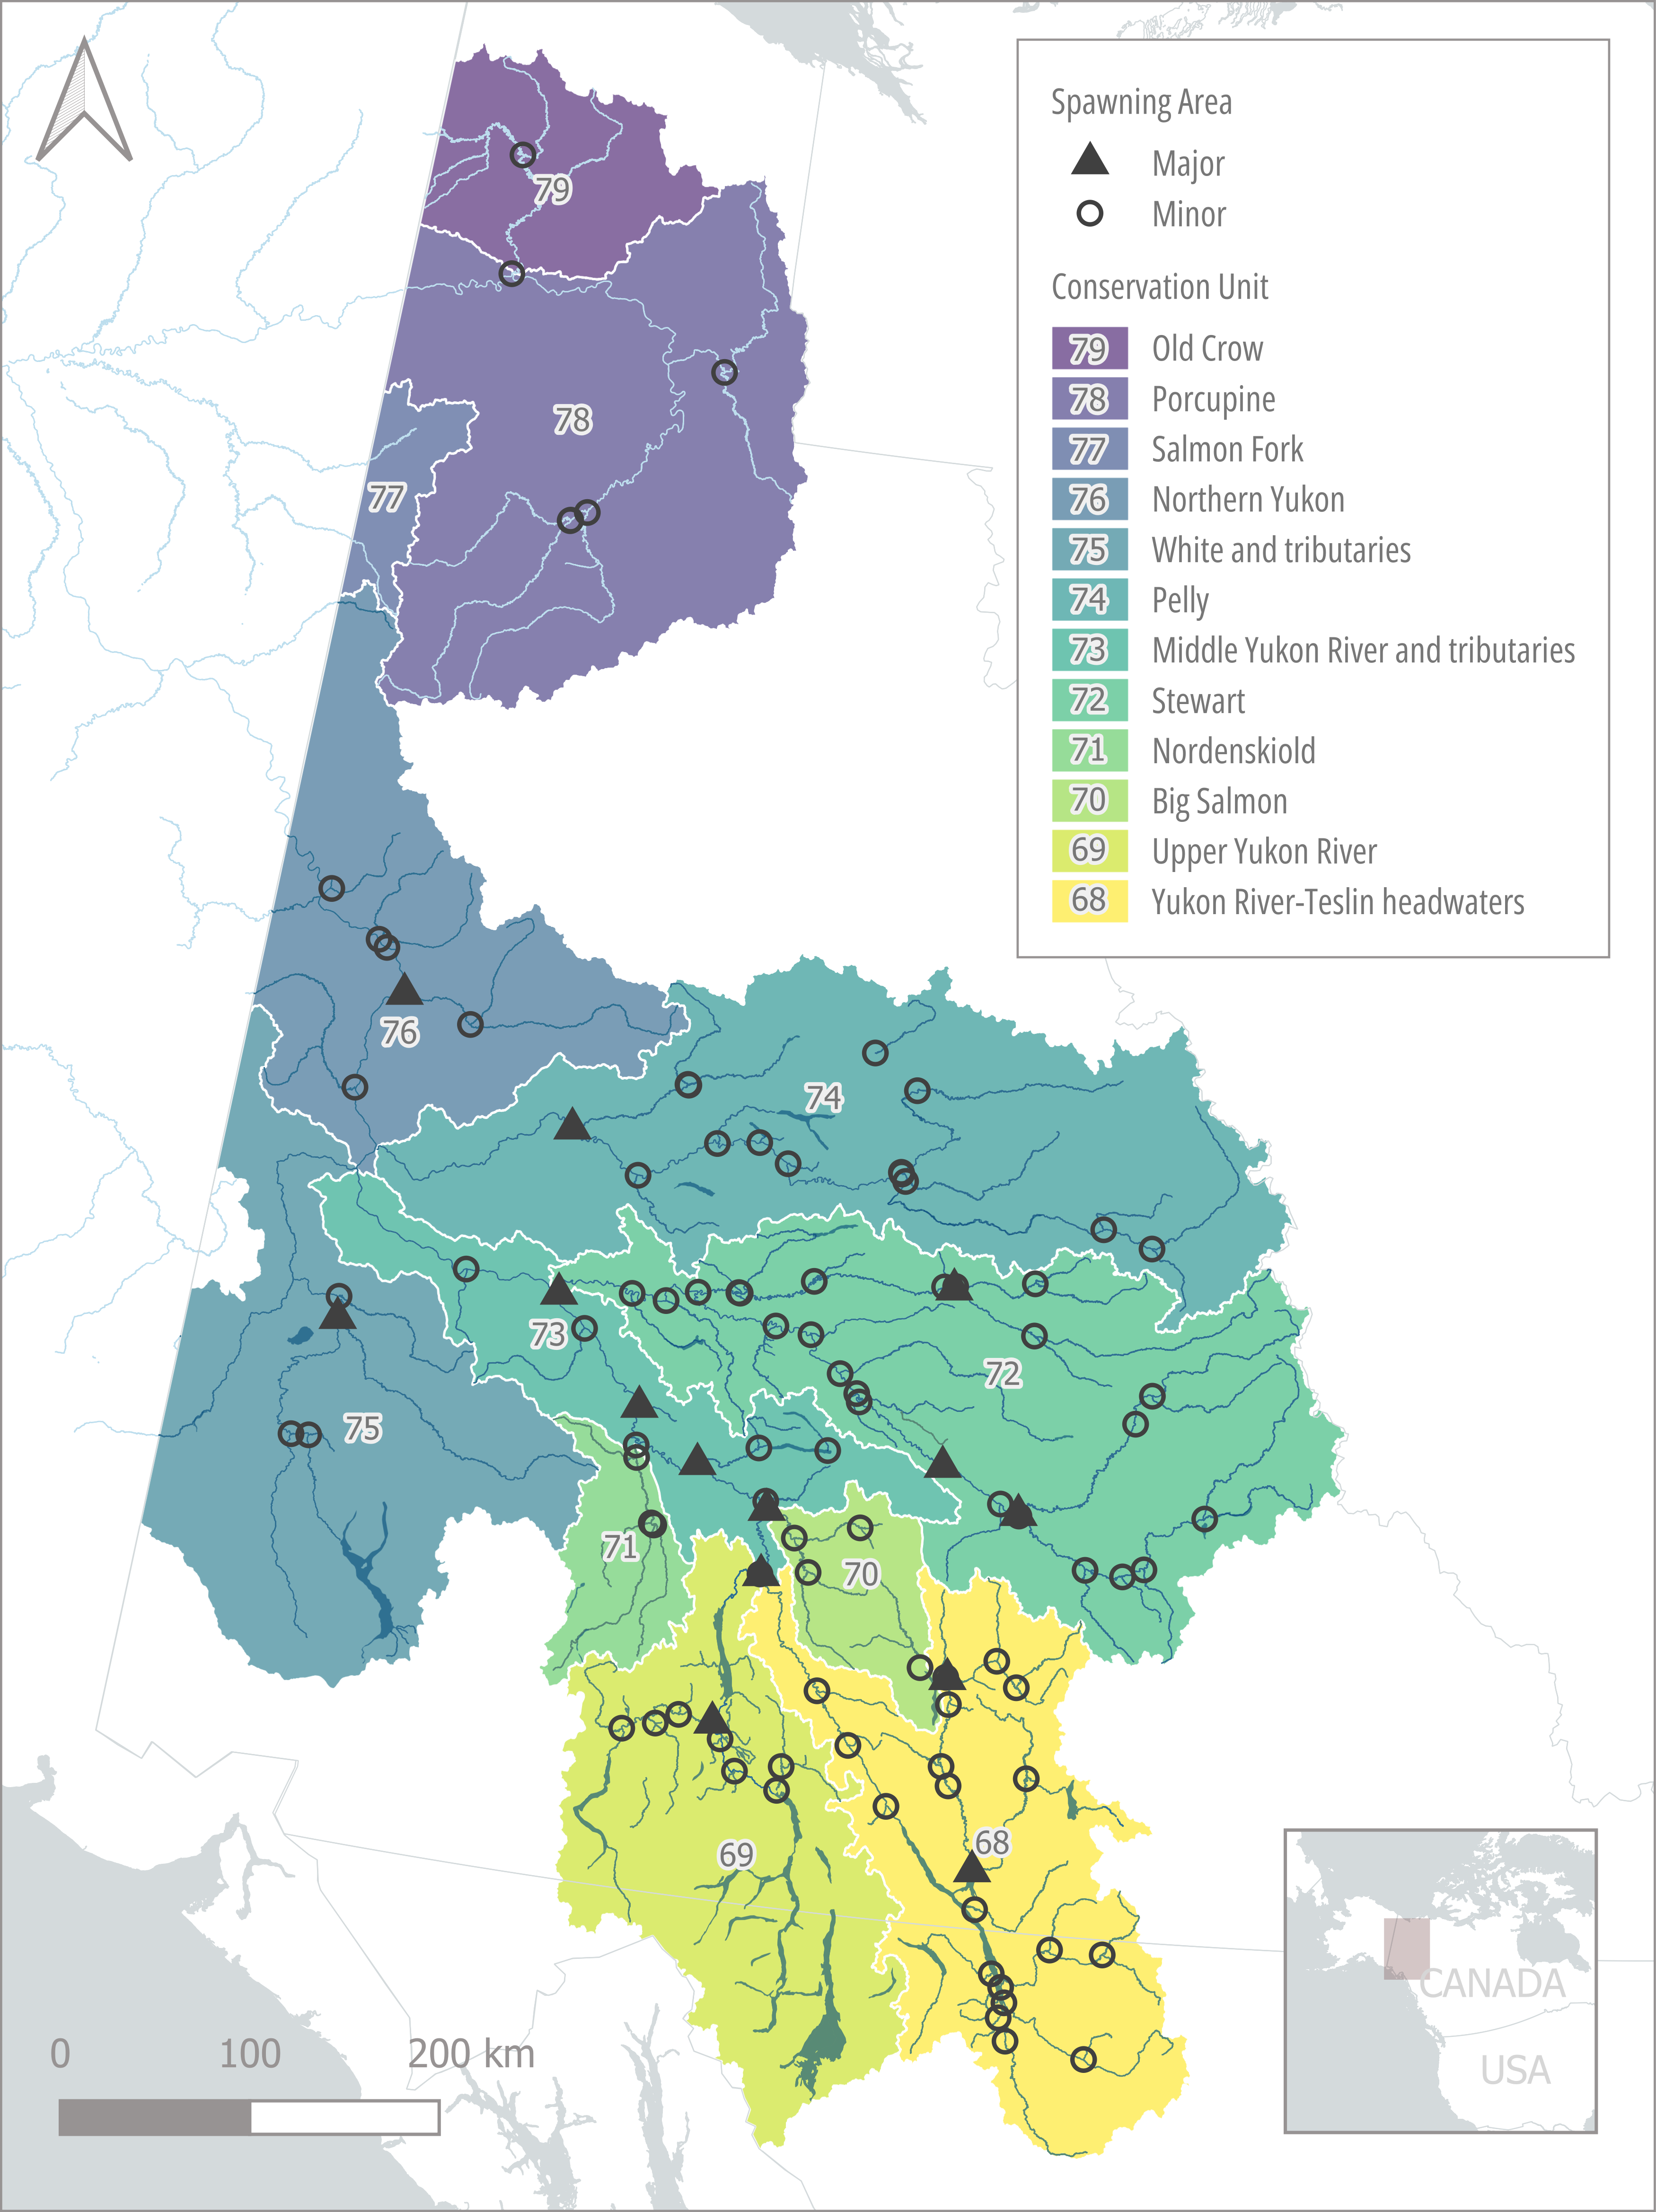
\includegraphics[width=6in]{figure/yukon-map-spawn}}{Figure \ref{fig:fig-map-spawn}} 

}

\caption{Canadian Yukon Chinook salmon Conservation Units and major and minor spawning locations as cataloged in Brown et al. (\protect\hyperlink{ref-brown_catalog_2017}{2017a}).}\label{fig:fig-map-spawn}
\end{figure}

\begin{figure}[htb]

{\centering \pdftooltip{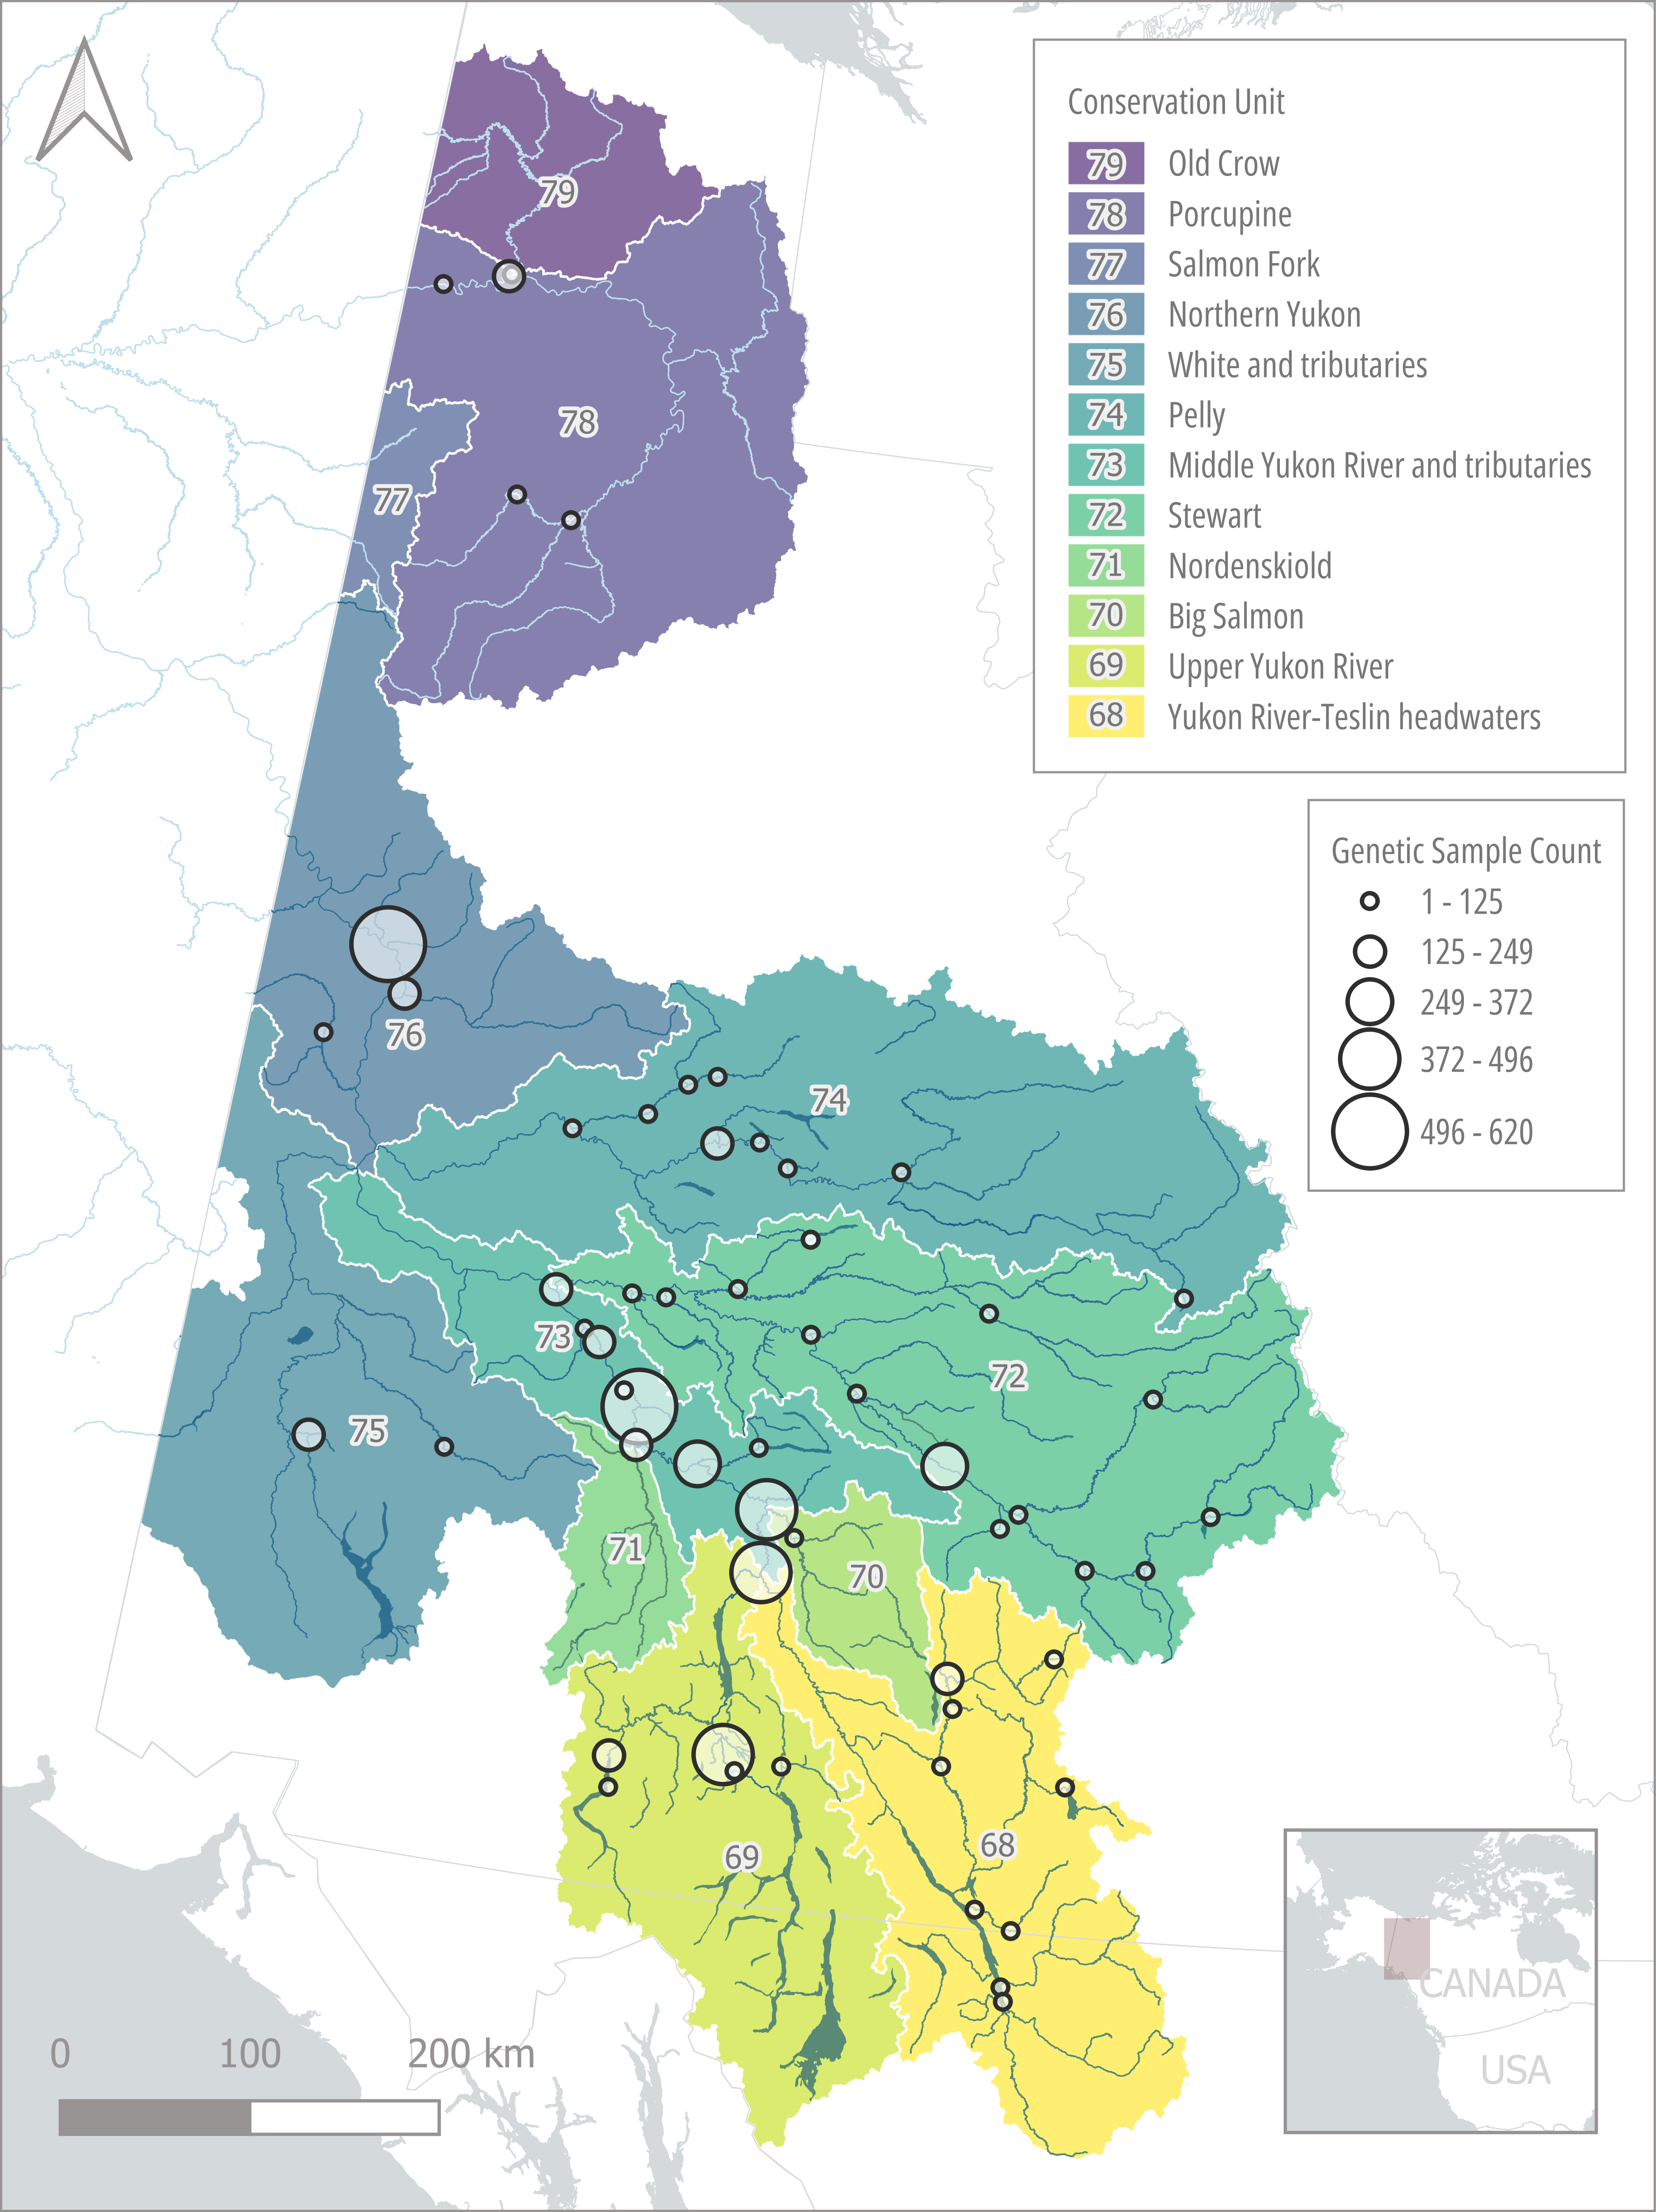
\includegraphics[width=6in]{figure/yukon-map-gsi}}{Figure \ref{fig:fig-map-gsi}} 

}

\caption{Various assessment sites and genetics sampling locations and number of samples per site in the Canadian portion of the Yukon River watershed.}\label{fig:fig-map-gsi}
\end{figure}

\begin{figure}[htb]

{\centering \pdftooltip{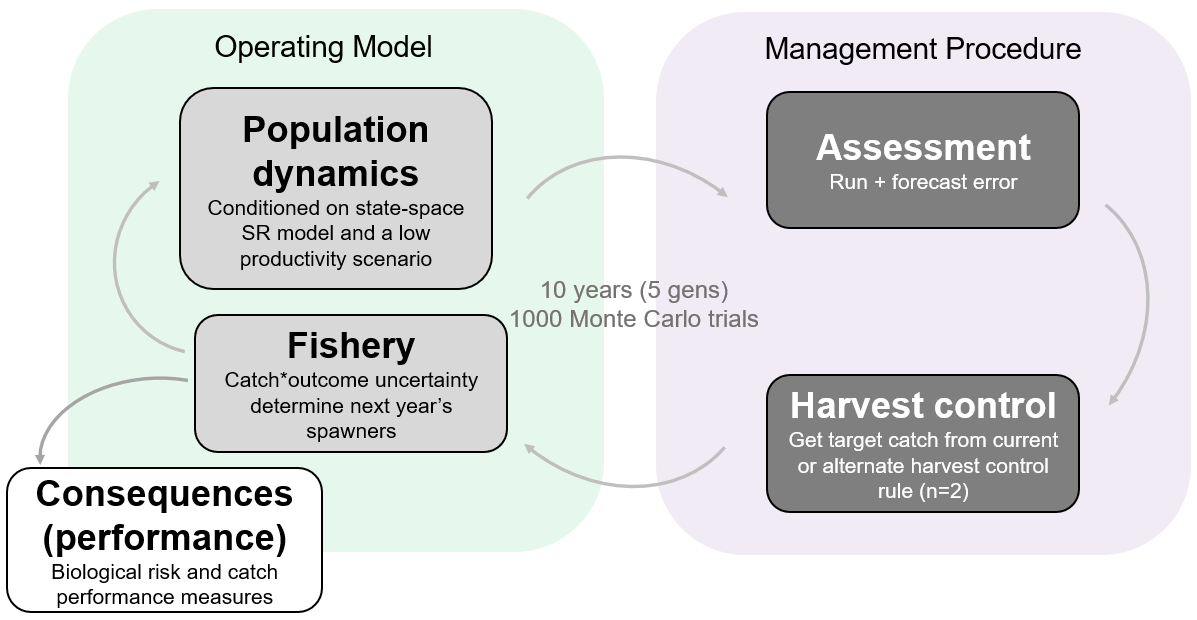
\includegraphics[width=6in]{figure/fwd-sim-schematic}}{Figure \ref{fig:fig-schematic}} 

}

\caption{Illustration of steps in the forward simulation highlighting alternate scenarios in population dynamics and harvest control rules.}\label{fig:fig-schematic}
\end{figure}

\begin{figure}[htb]

{\centering \pdftooltip{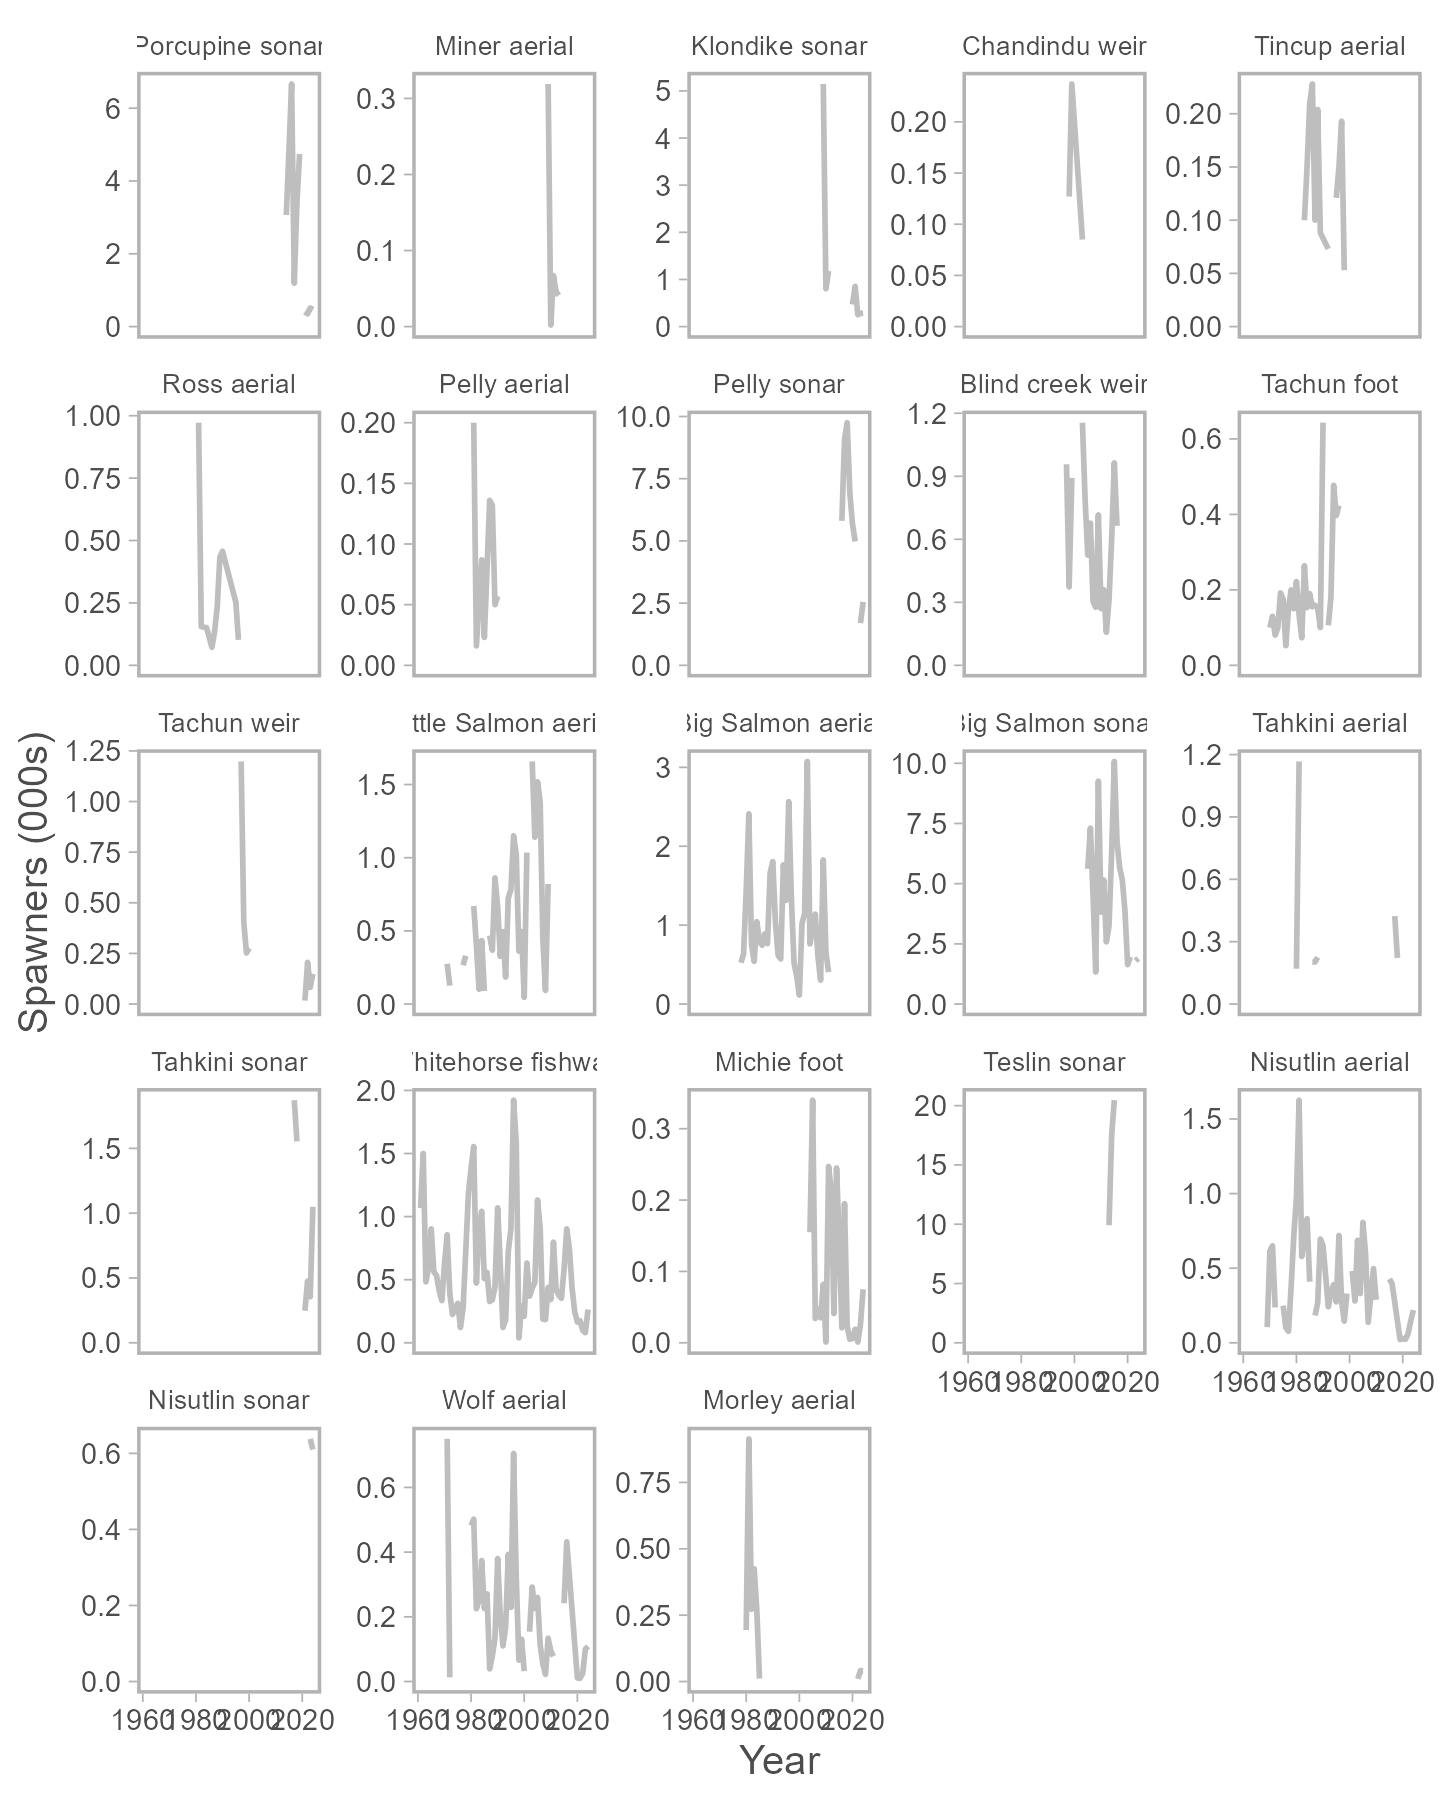
\includegraphics[width=6in]{figure/trib-escape}}{Figure \ref{fig:fig-trib-spawn}} 

}

\caption{Spawner abundances over time by tributary assessment project.}\label{fig:fig-trib-spawn}
\end{figure}

\begin{figure}[htb]

{\centering \pdftooltip{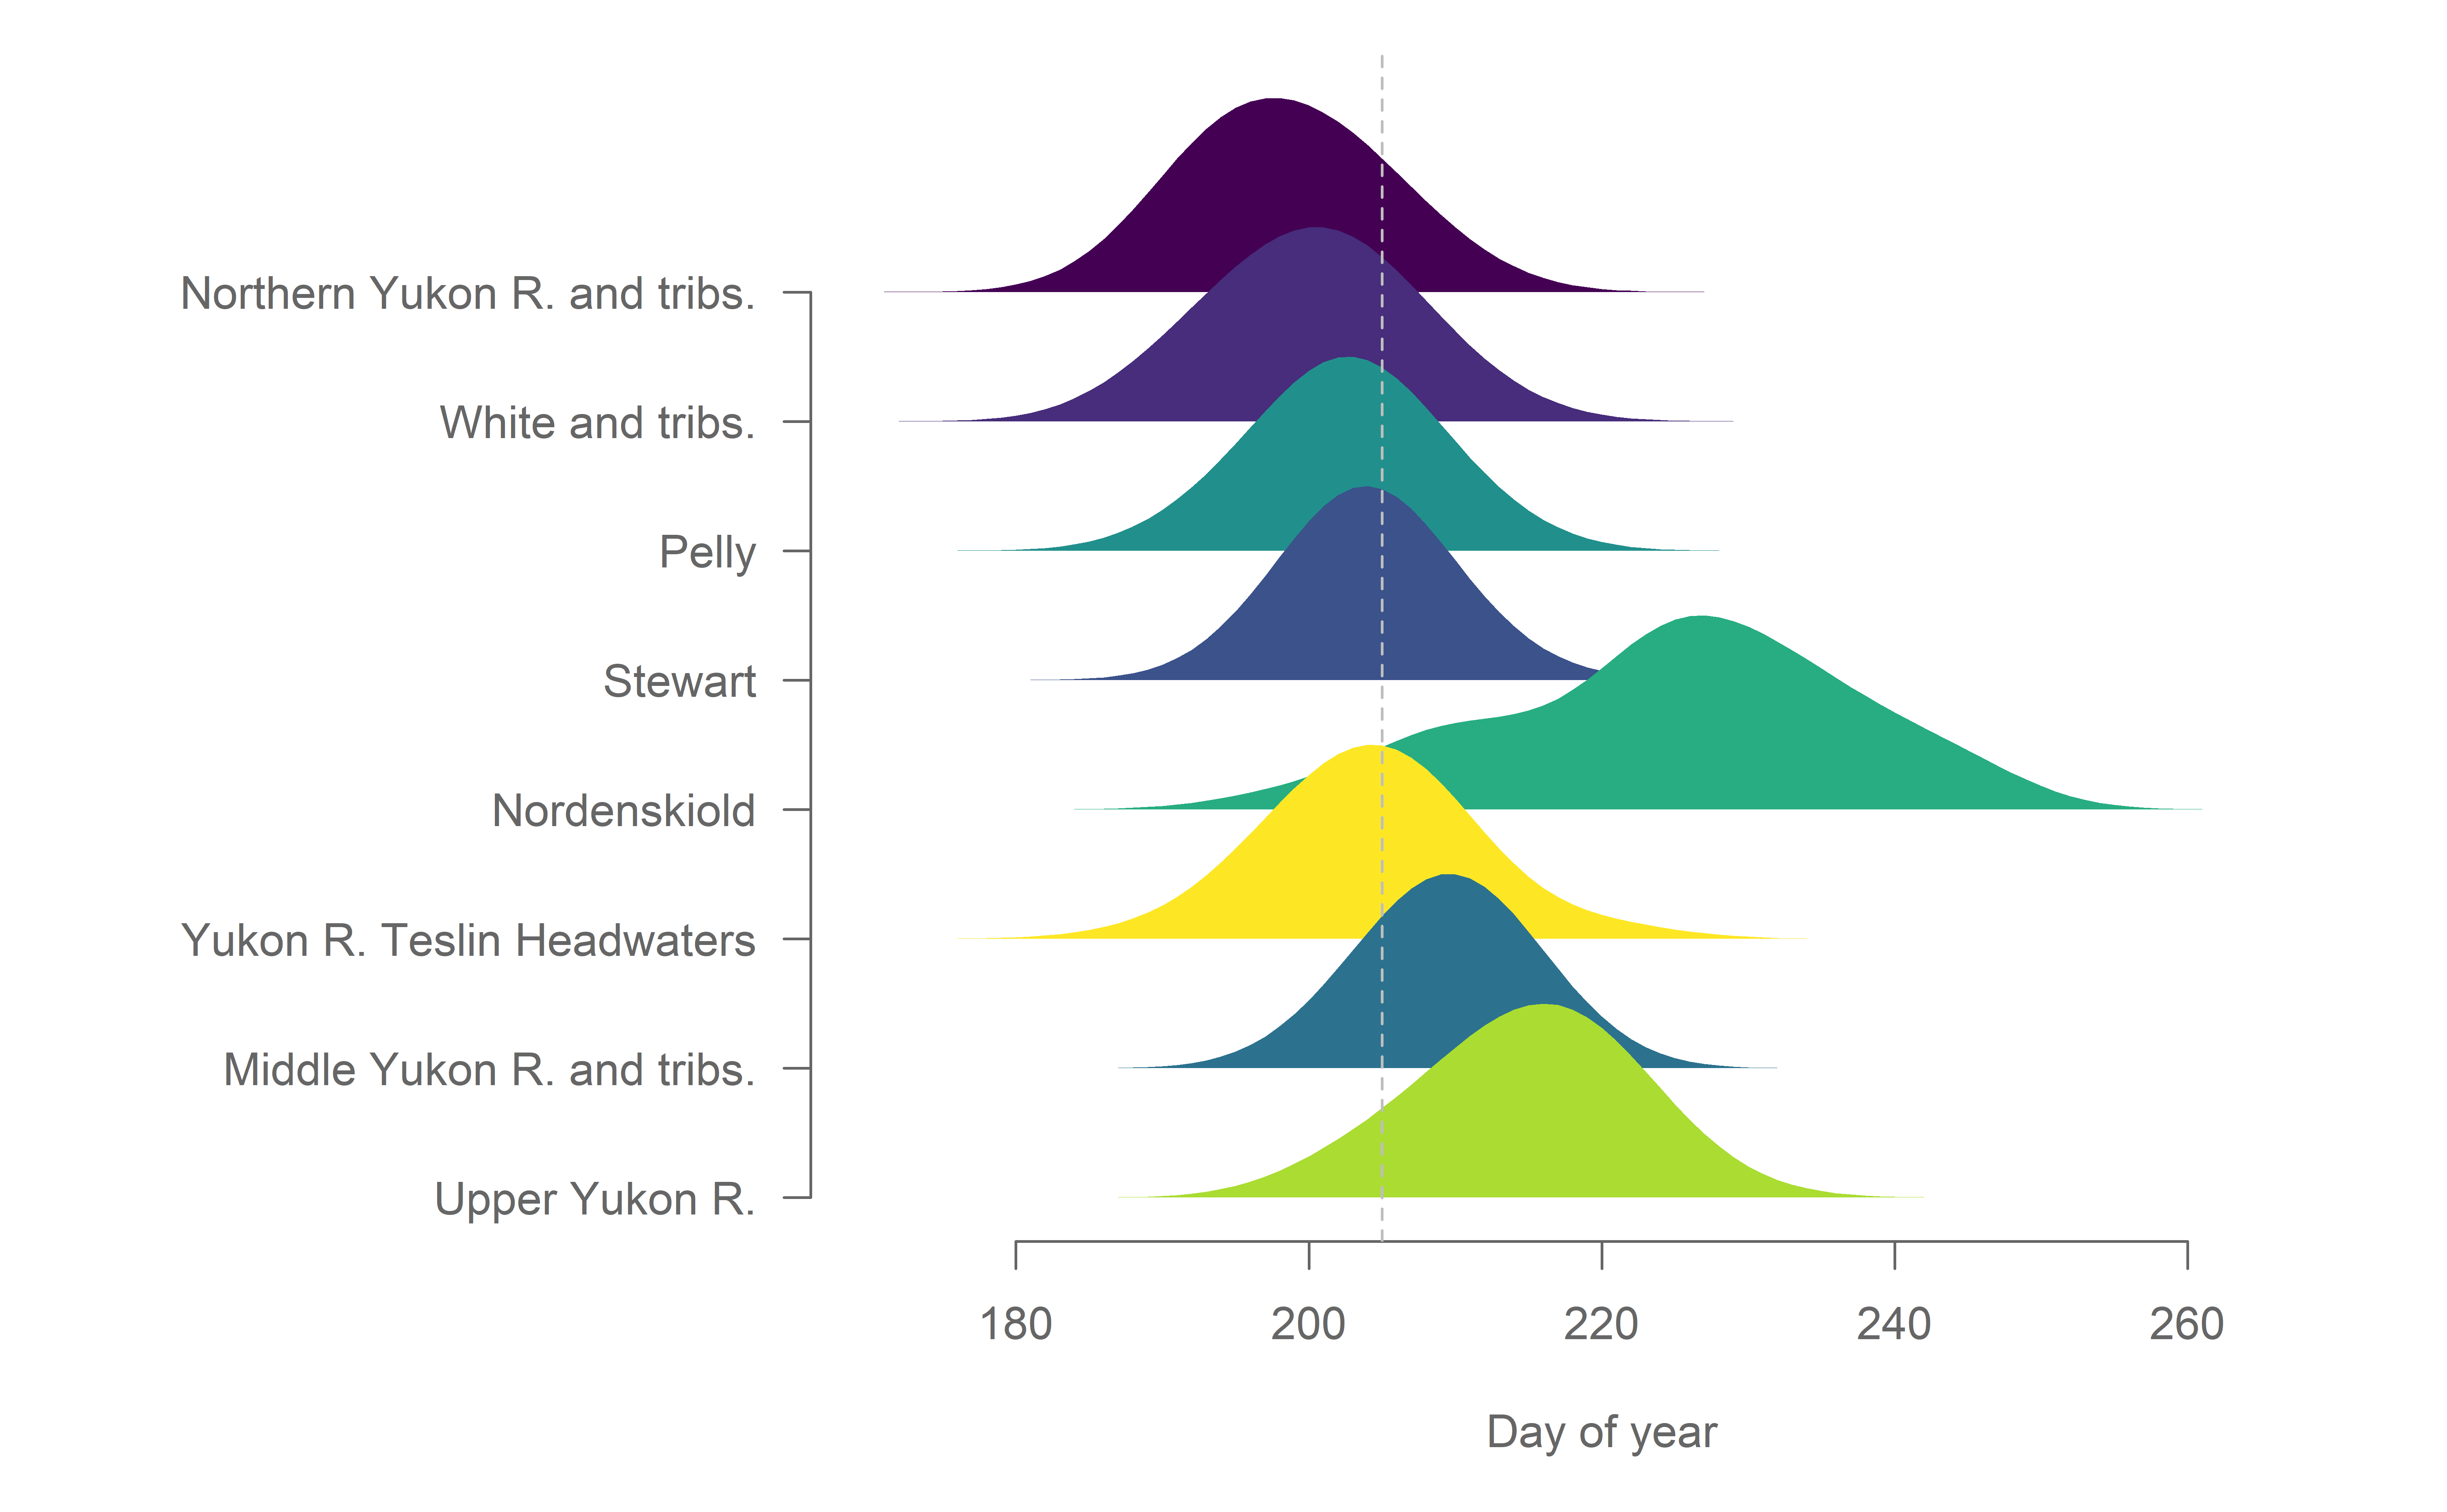
\includegraphics[width=6in]{figure/CU-run-timing}}{Figure \ref{fig:fig-run-timing}} 

}

\caption{Run-timing, at border, by CU.}\label{fig:fig-run-timing}
\end{figure}

\begin{figure}[htb]

{\centering \pdftooltip{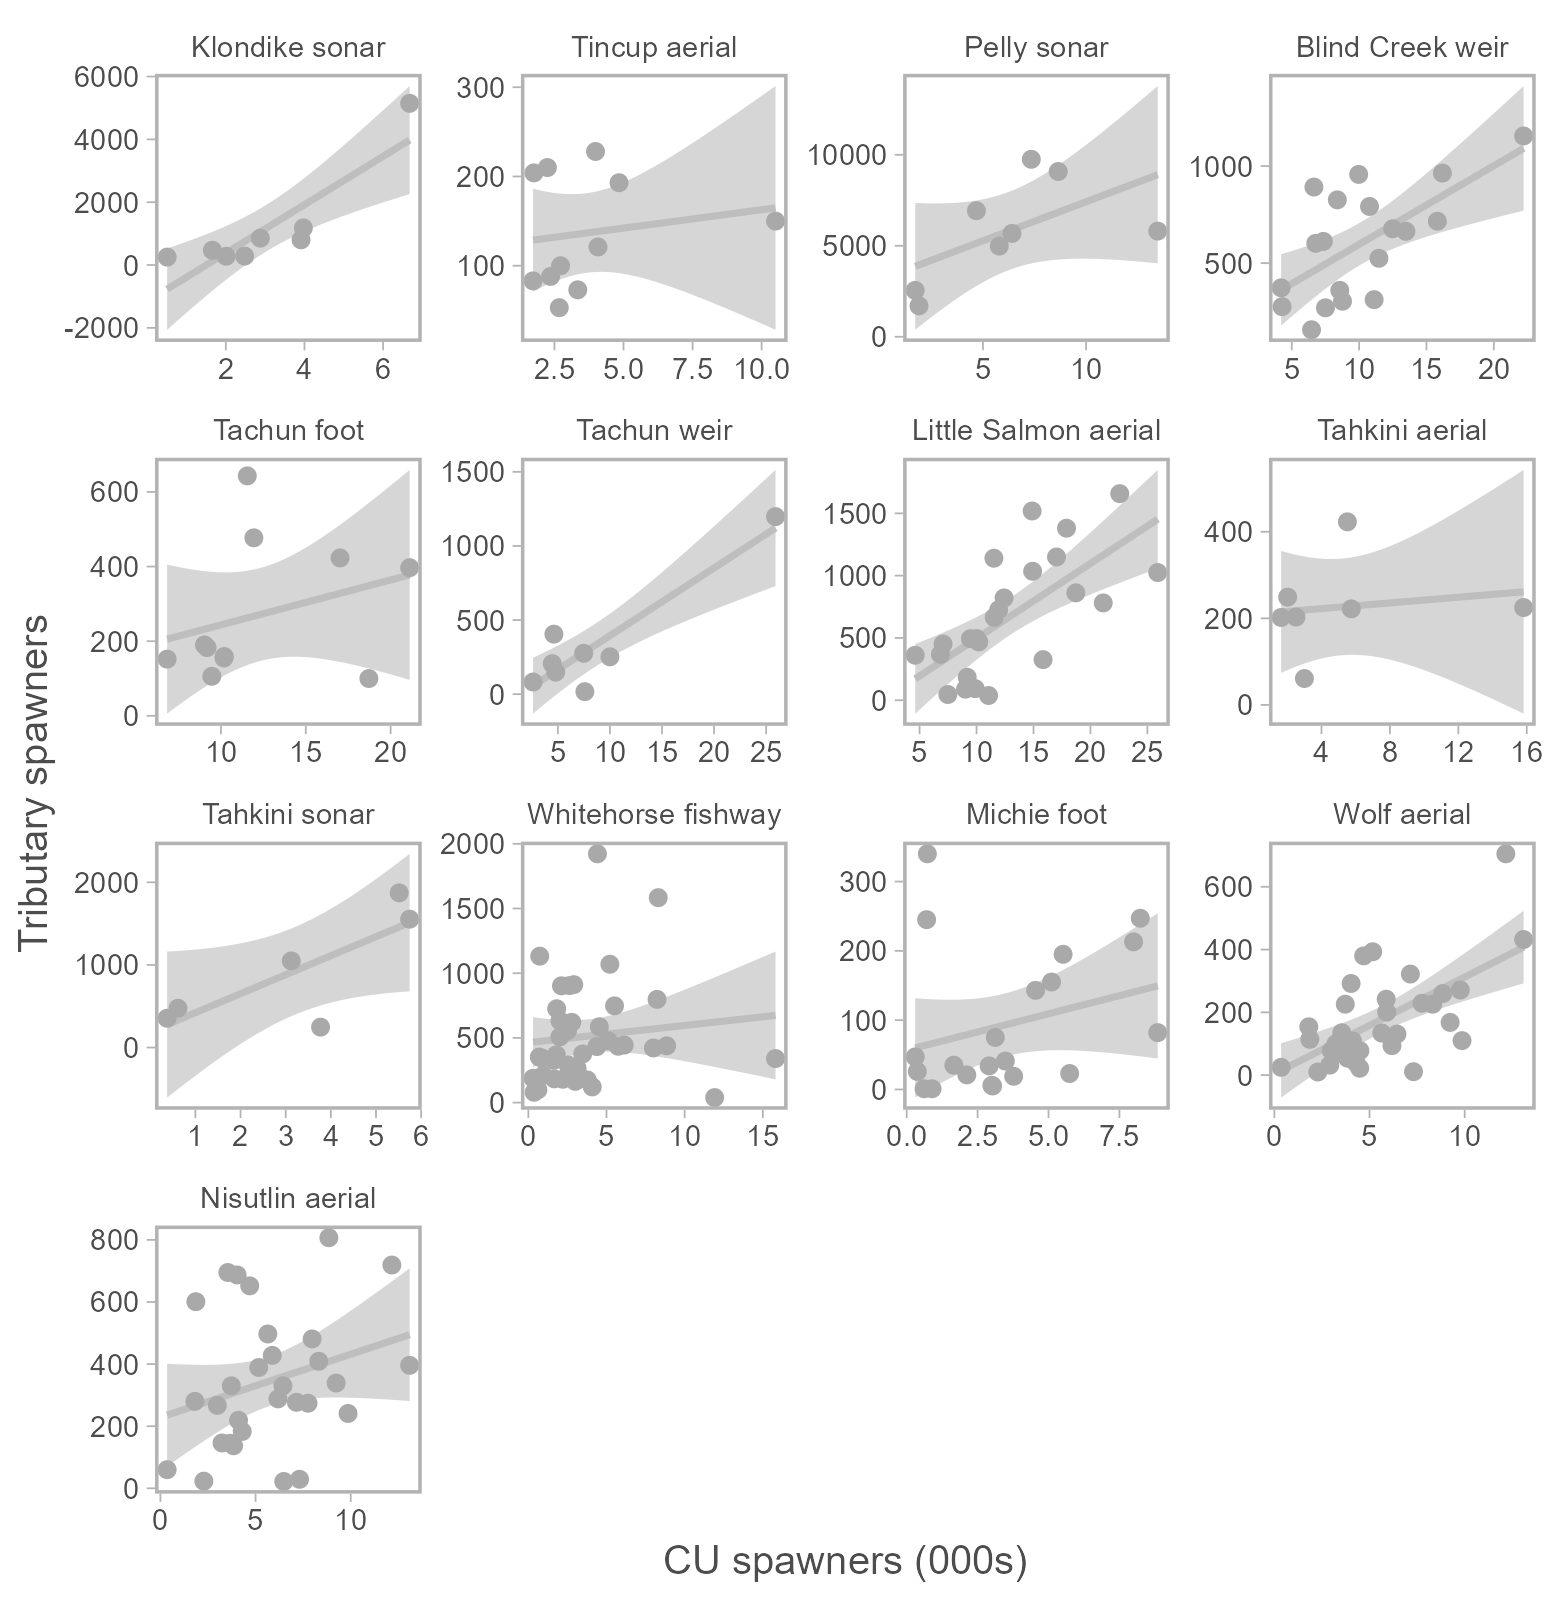
\includegraphics[width=6in]{figure/RR-vs-trib-spawners}}{Figure \ref{fig:fig-trib-vs-CU-spawn}} 

}

\caption{Tributary assessment project vs.~reconstructed spawner abundance over time.}\label{fig:fig-trib-vs-CU-spawn}
\end{figure}

\begin{figure}[htb]

{\centering \pdftooltip{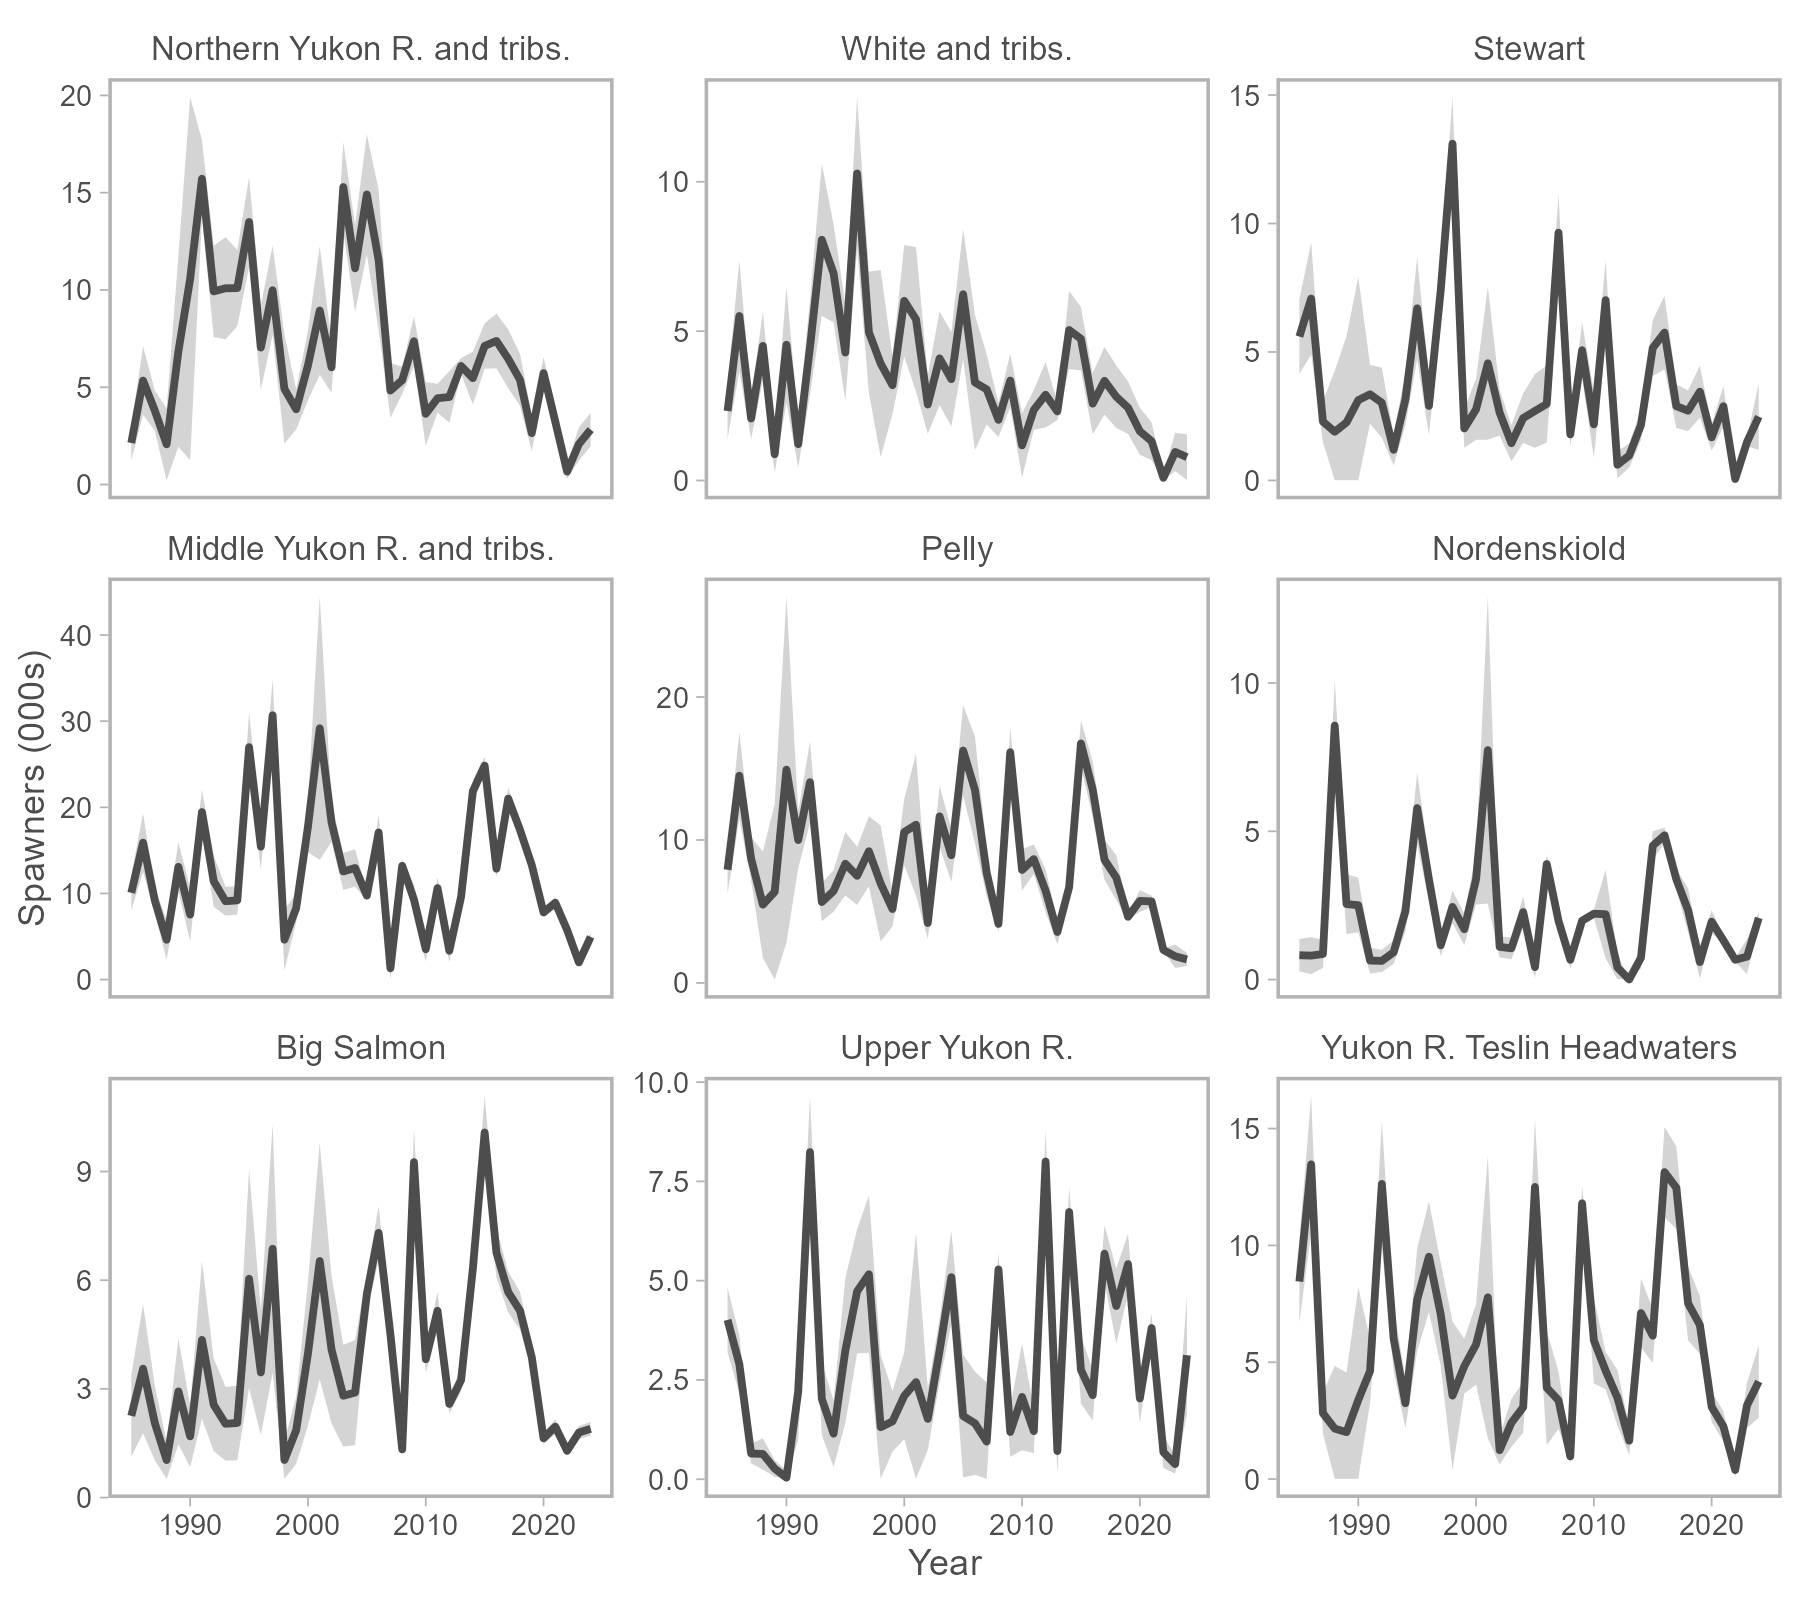
\includegraphics[width=6in]{figure/cu-escape}}{Figure \ref{fig:fig-CU-spawn}} 

}

\caption{Reconstructed spawner abundance over time by CU.}\label{fig:fig-CU-spawn}
\end{figure}

\begin{figure}[htb]

{\centering \pdftooltip{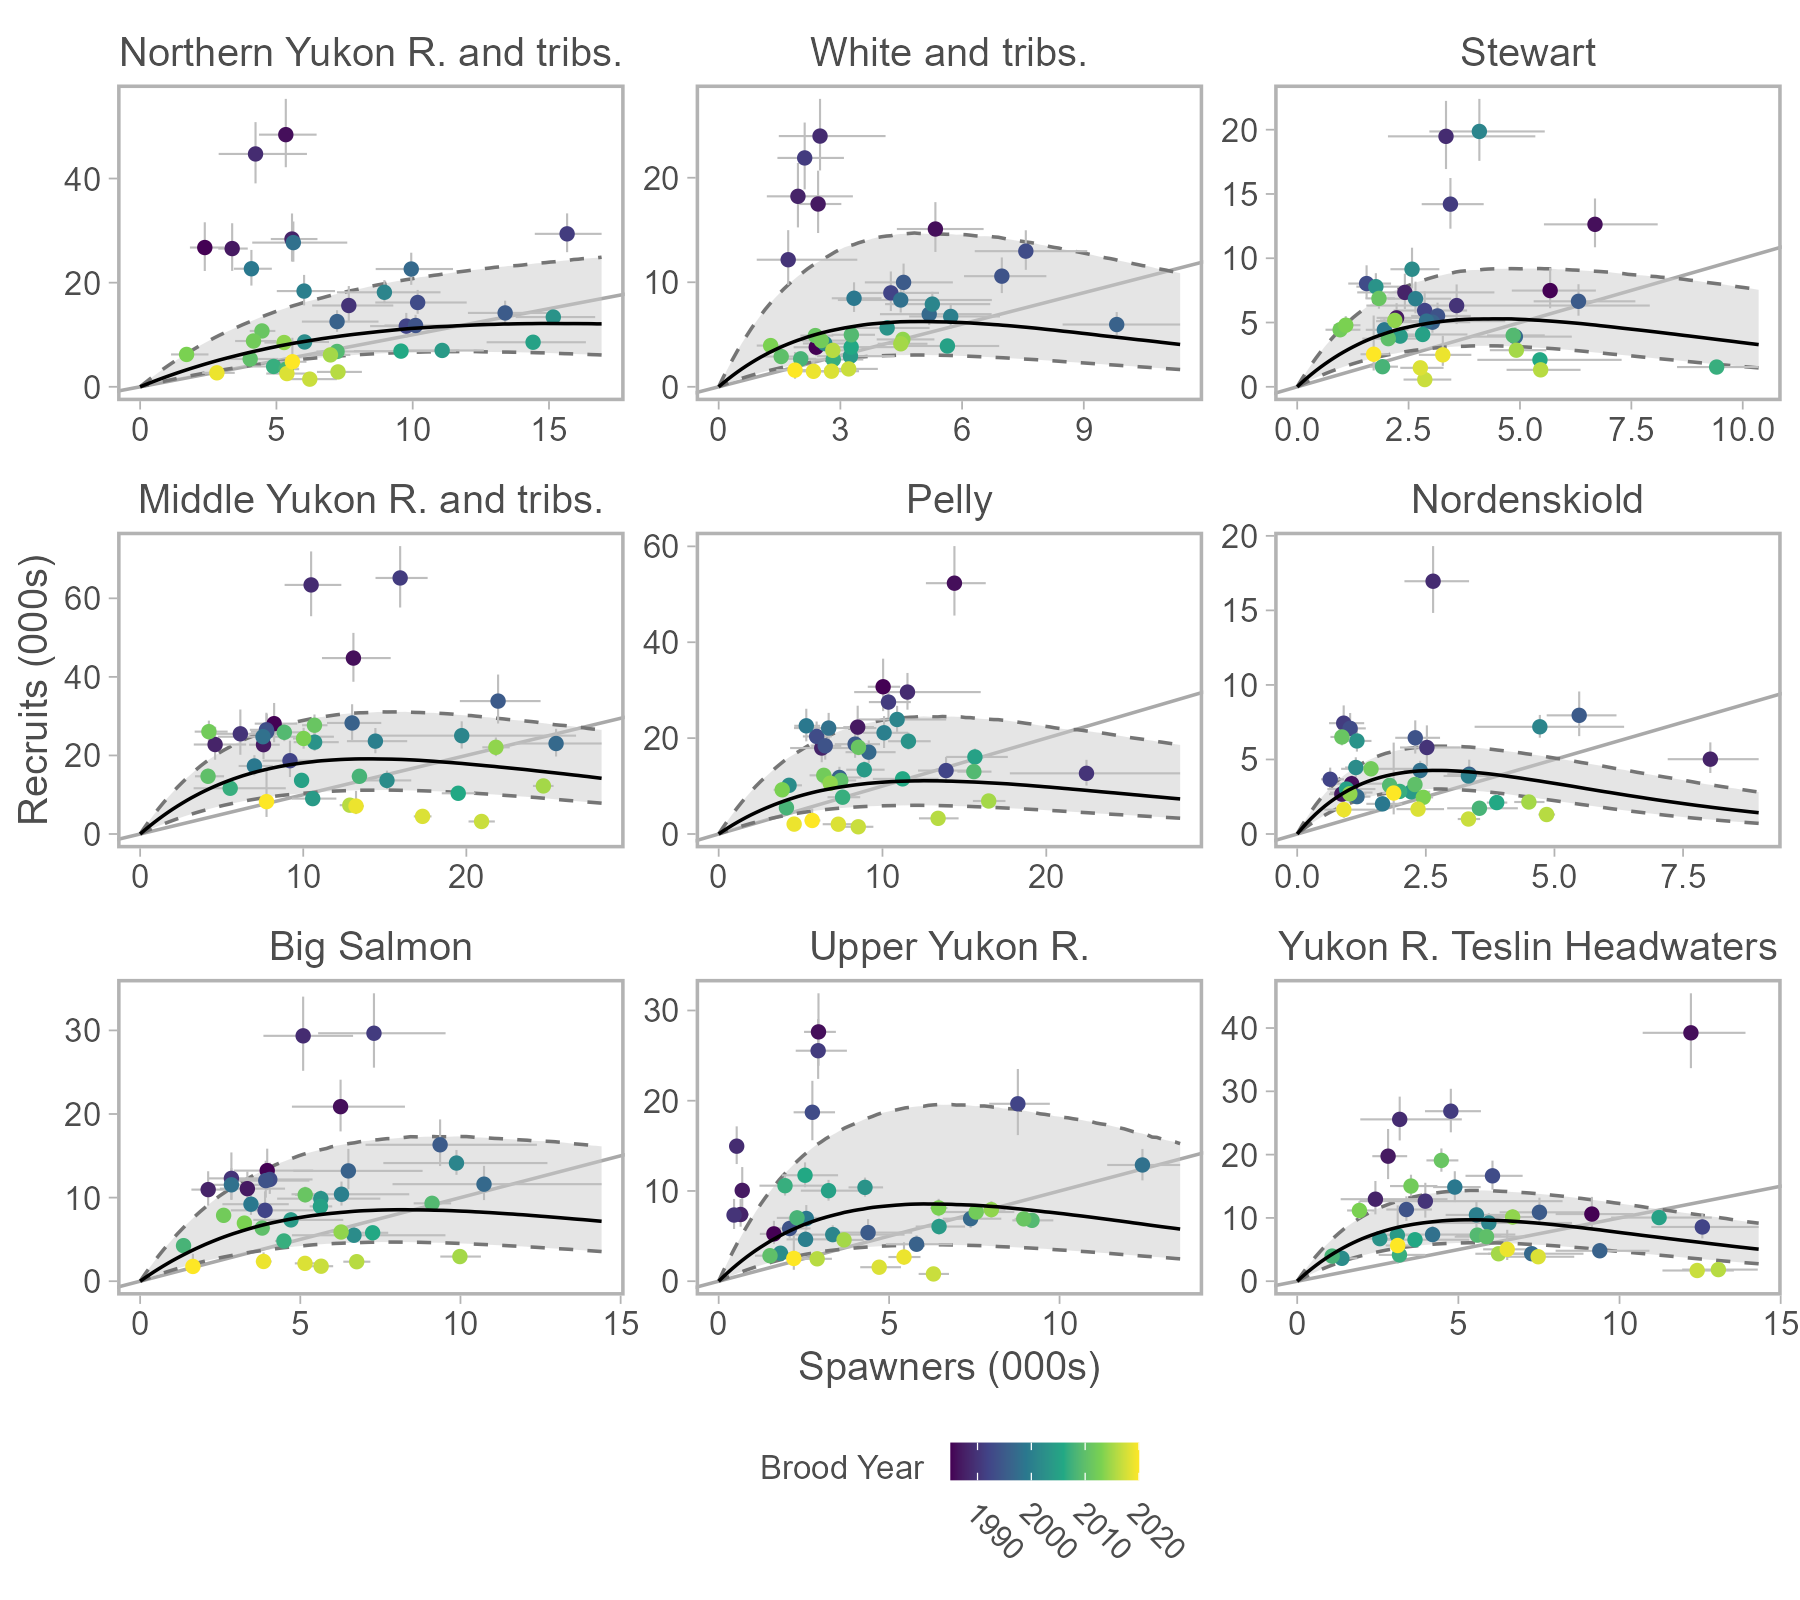
\includegraphics[width=6in]{figure/SR_fits_AR1}}{Figure \ref{fig:fig-CU-SR}} 

}

\caption{Spawner recruitment relationships by CU.}\label{fig:fig-CU-SR}
\end{figure}

\begin{figure}[htb]

{\centering \pdftooltip{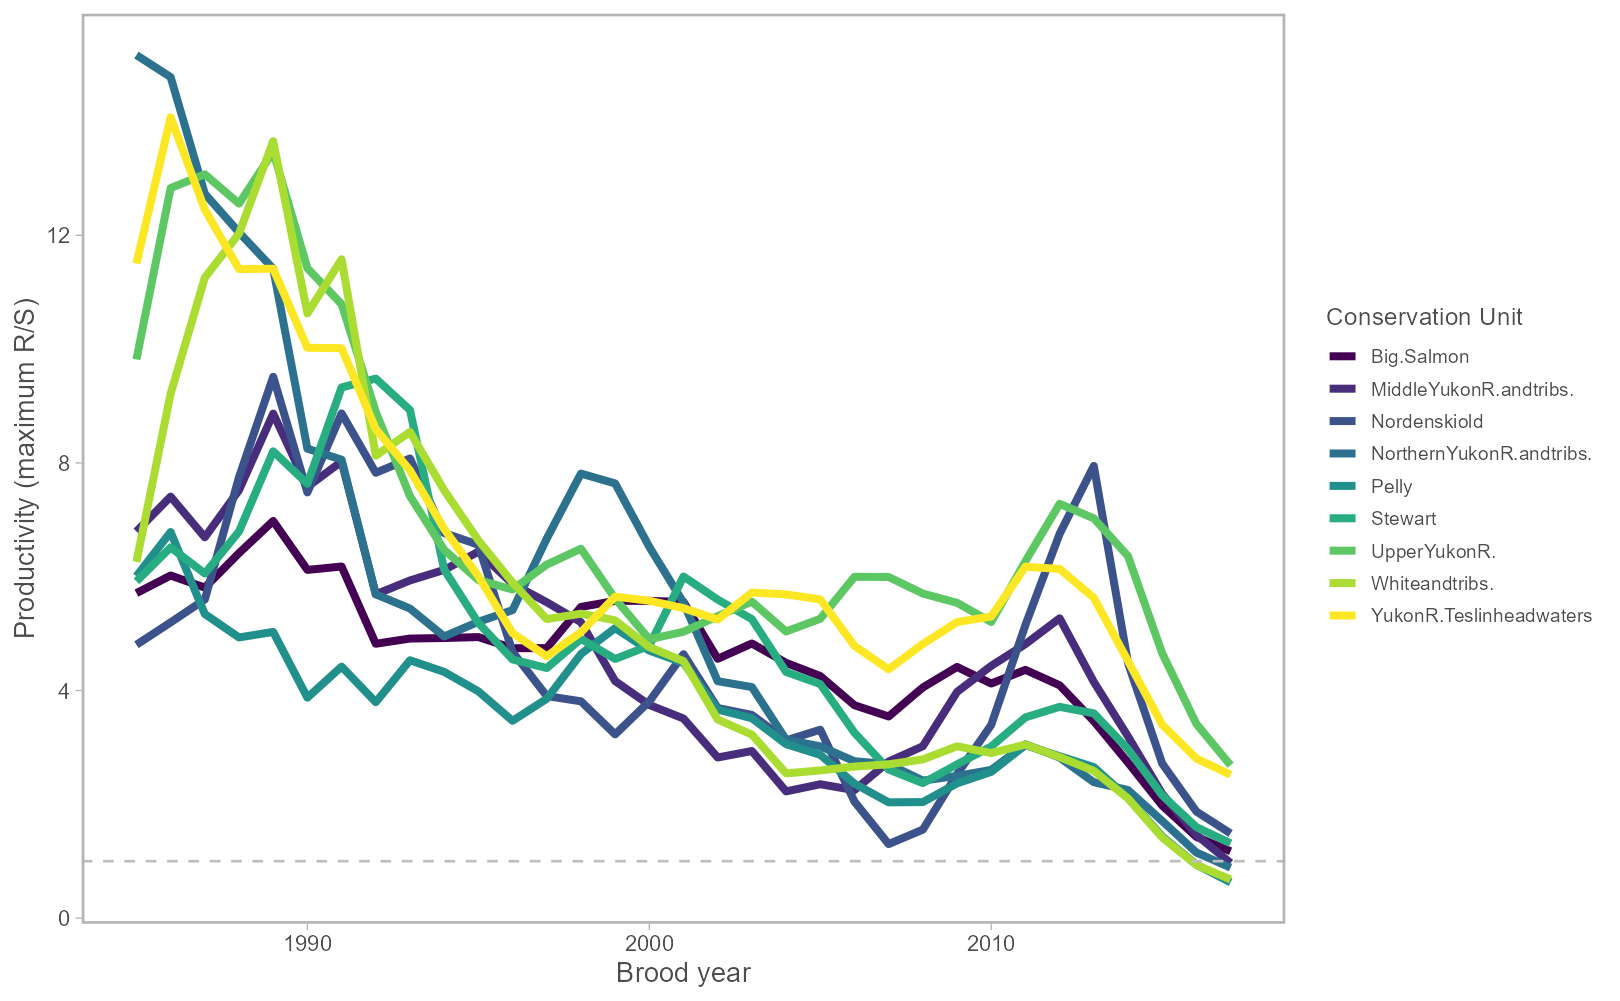
\includegraphics[width=6in]{figure/changing_productivity}}{Figure \ref{fig:fig-prod-trends}} 

}

\caption{Trends in intrinsic productivity over time by CU.}\label{fig:fig-prod-trends}
\end{figure}

\begin{figure}[htb]

{\centering \pdftooltip{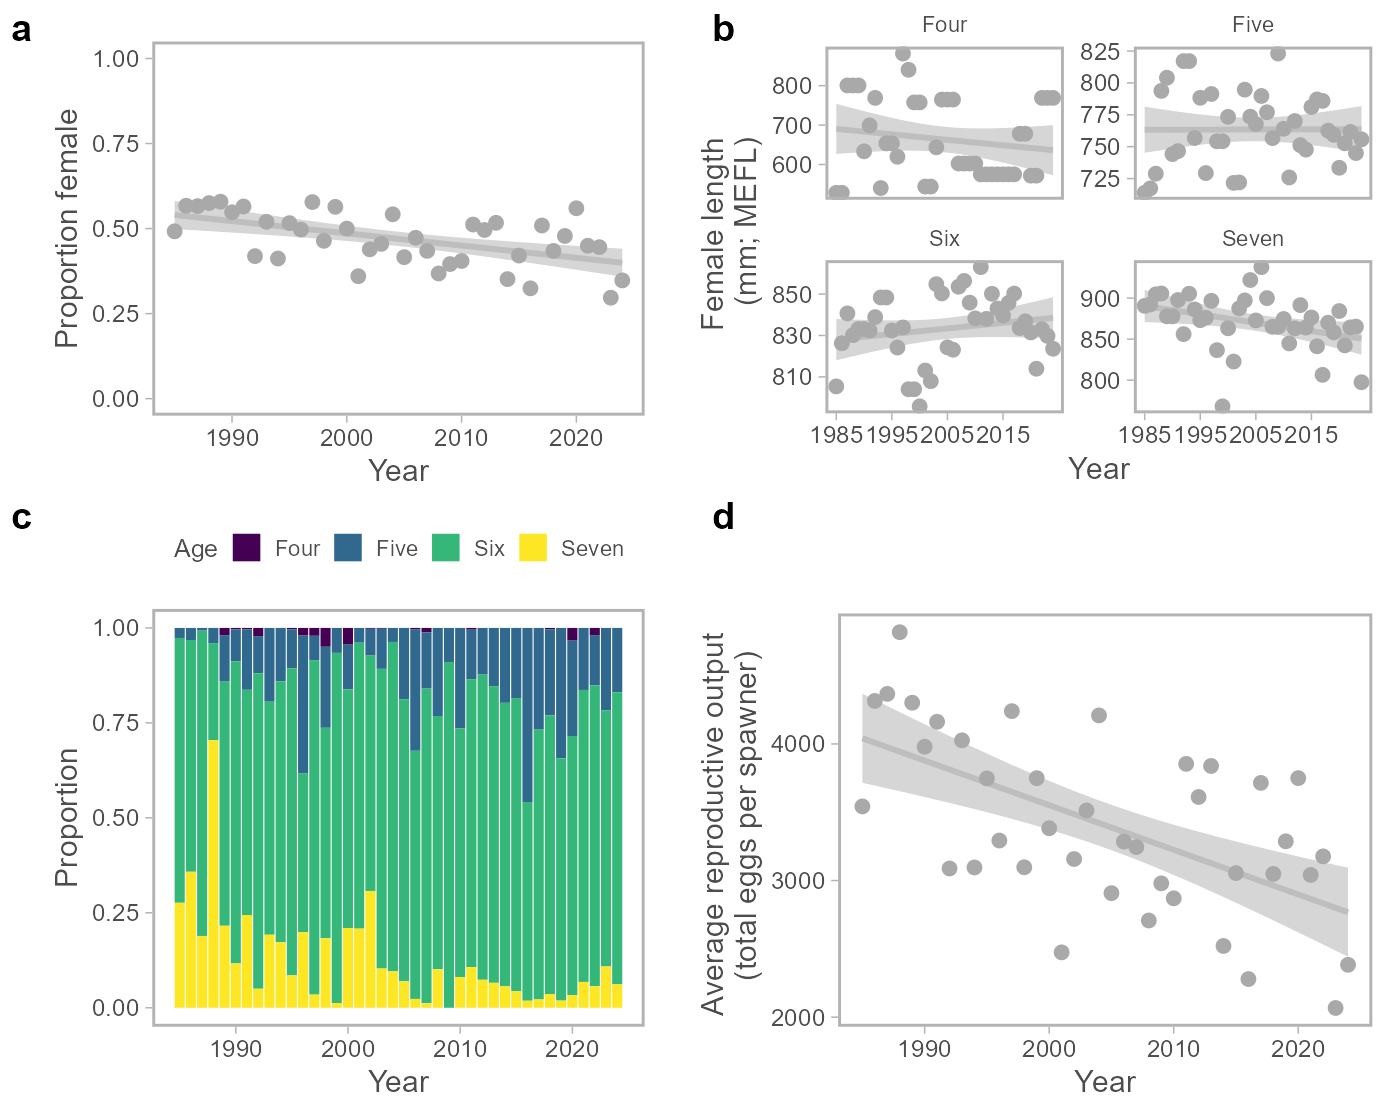
\includegraphics[width=6in]{figure/asl}}{Figure \ref{fig:fig-asl}} 

}

\caption{Trends in asl over time.}\label{fig:fig-asl}
\end{figure}

\begin{figure}[htb]

{\centering \pdftooltip{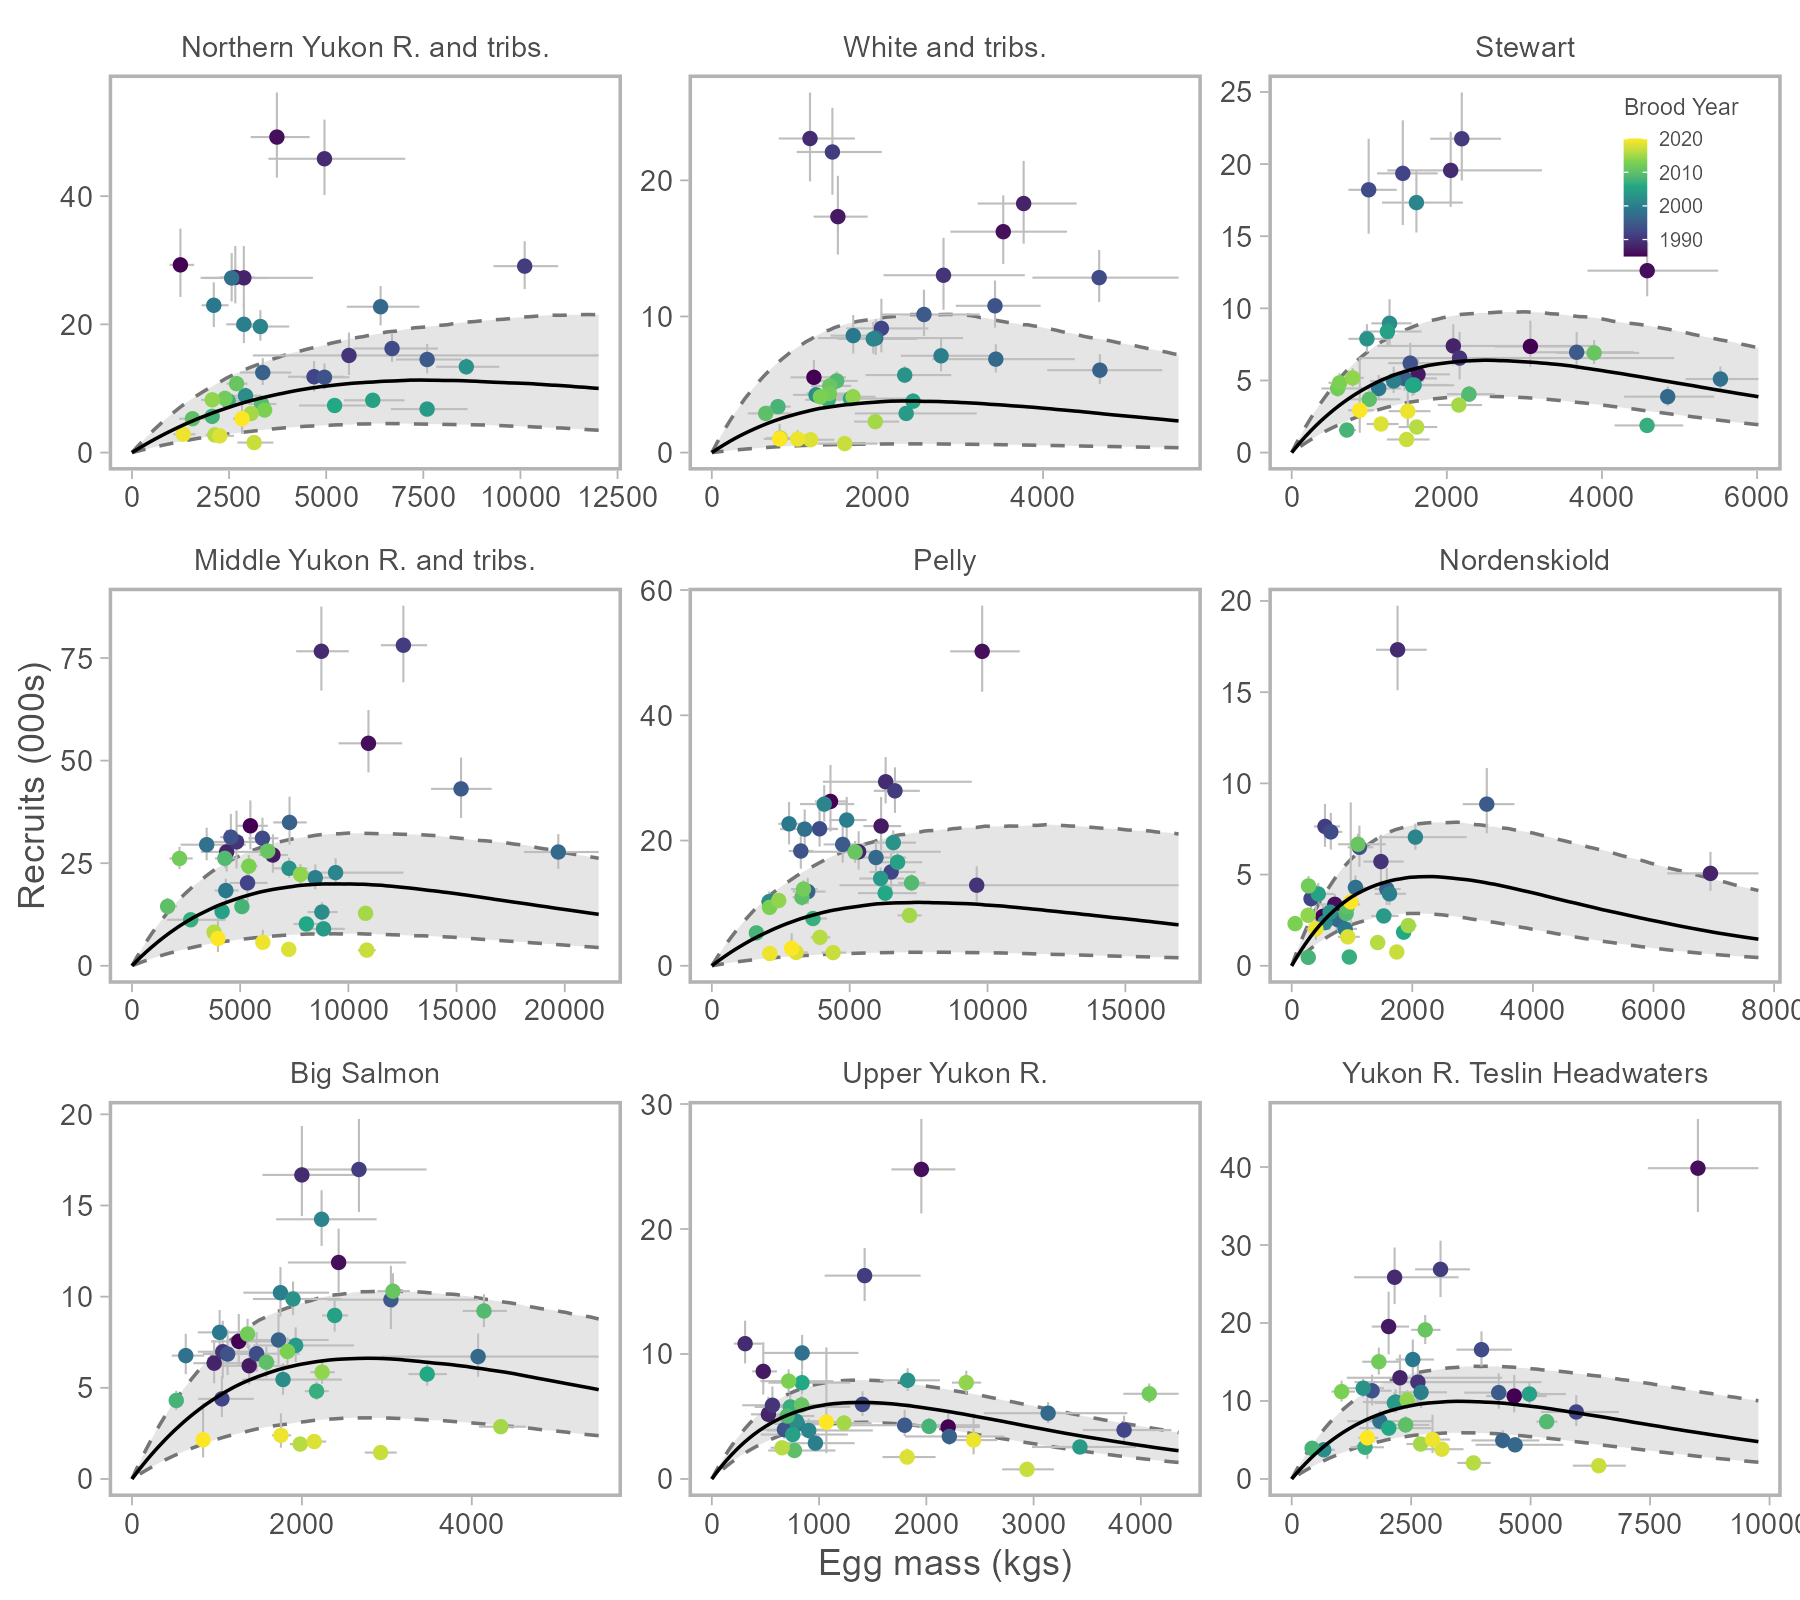
\includegraphics[width=6in]{figure/EM-R_fits}}{Figure \ref{fig:fig-CU-EMR}} 

}

\caption{Egg mass recruitment relationships by CU.}\label{fig:fig-CU-EMR}
\end{figure}

\begin{figure}[htb]

{\centering \pdftooltip{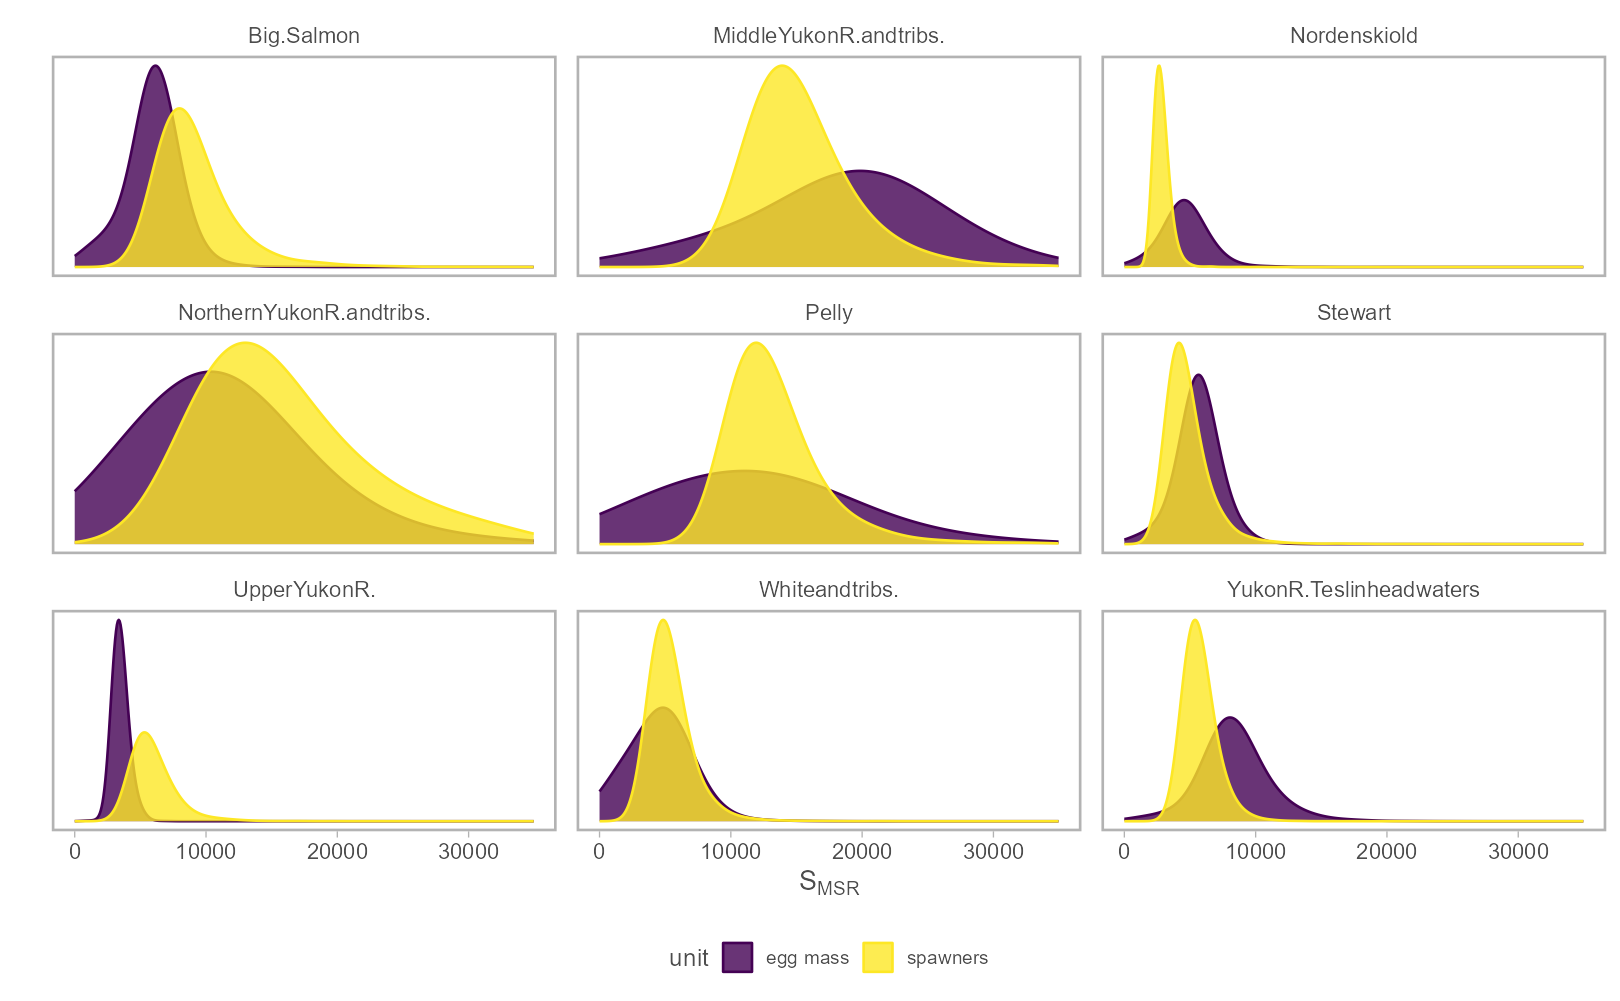
\includegraphics[width=6in]{figure/demo_bench_compare_spawn-vs-recent}}{Figure \ref{fig:fig-demo-smsr}} 

}

\caption{Egg mass recruitment relationships by CU.}\label{fig:fig-demo-smsr}
\end{figure}

\begin{figure}[htb]

{\centering \pdftooltip{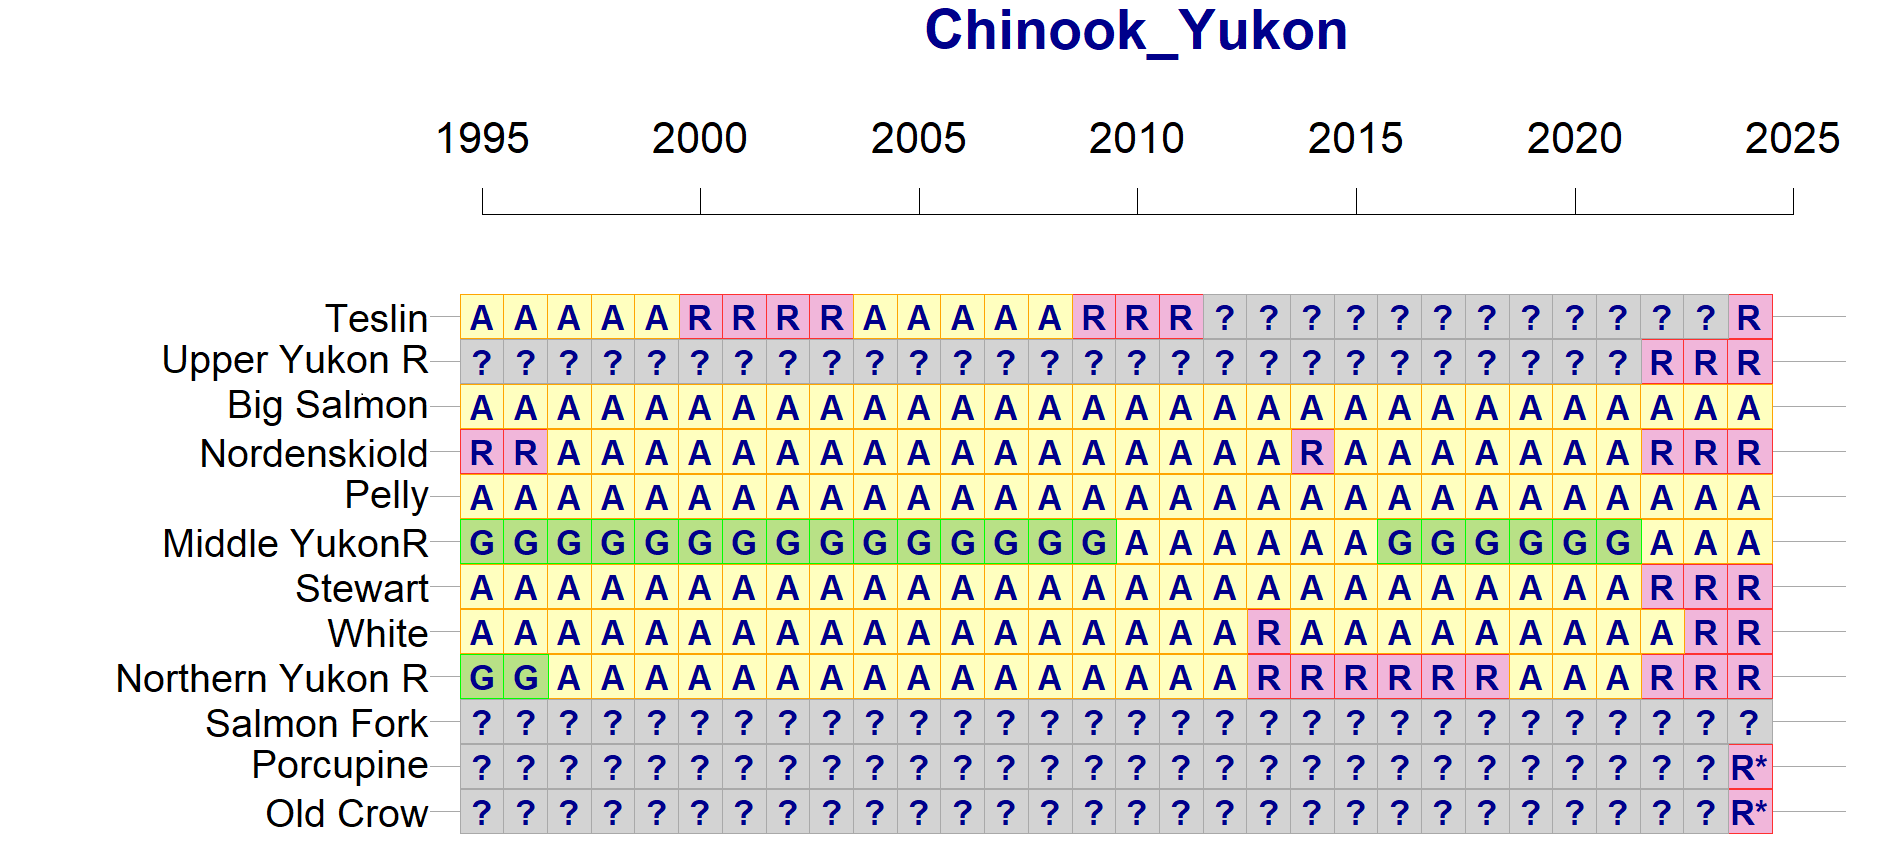
\includegraphics[width=6in]{figure/rapid-status}}{Figure \ref{fig:fig-rapid-status}} 

}

\caption{Yukon Chinook WSP rapid statuses for years with applicable data. Each row summarizes the rapid statuses available for each CU in this SMU.}\label{fig:fig-rapid-status}
\end{figure}

\begin{figure}[htb]

{\centering \pdftooltip{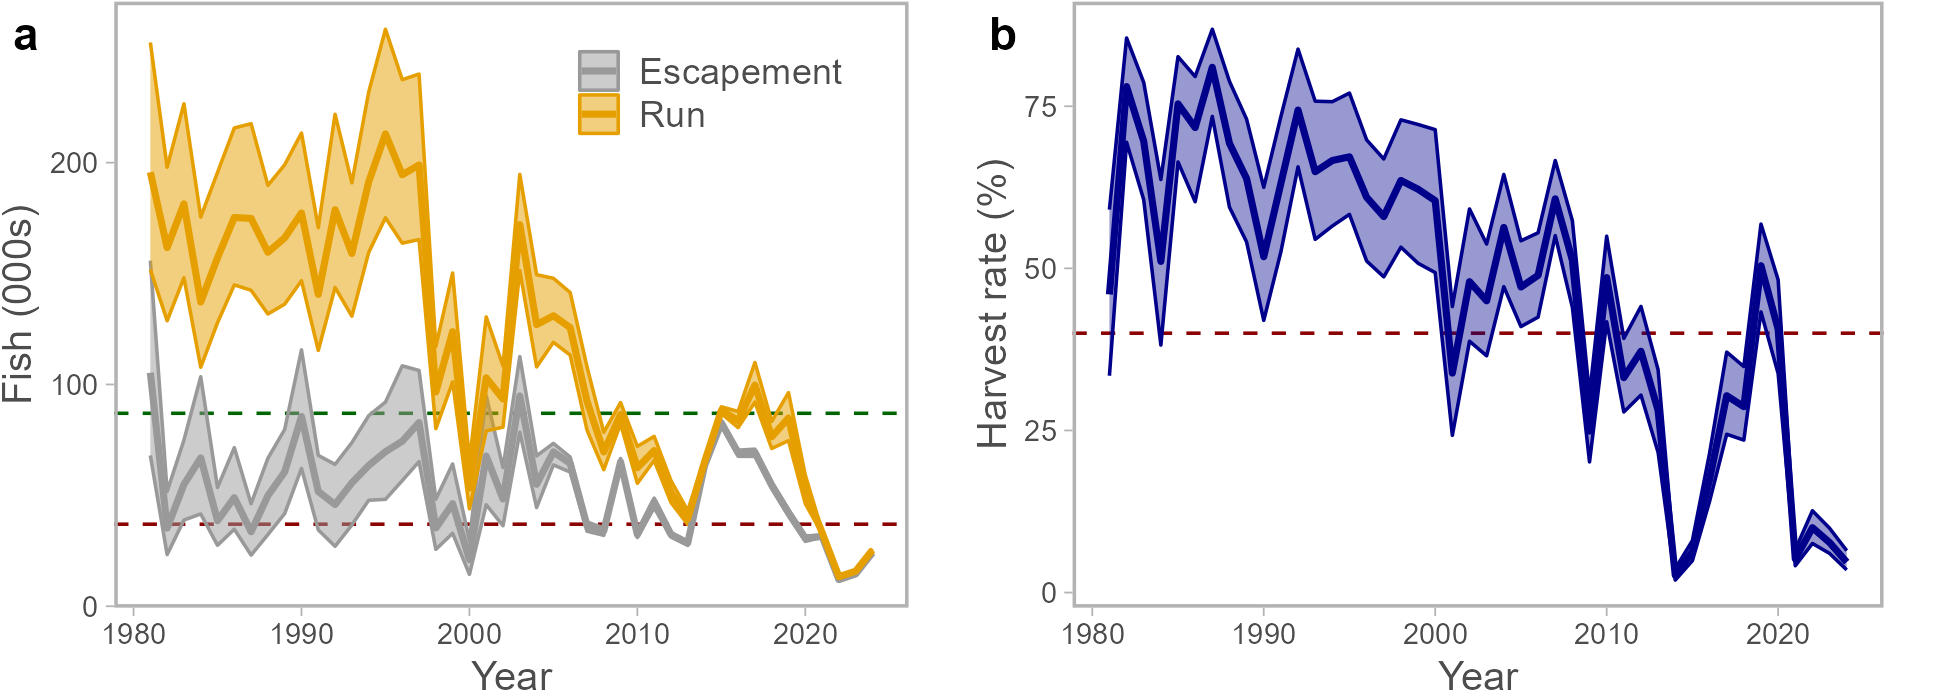
\includegraphics[width=6in]{figure/SMU-run-esc}}{Figure \ref{fig:fig-smu-trends}} 

}

\caption{Reconstructed (a) total run size (orange) and spawning escapement (grey), and (b) harvest rates for the Yukon River SMU. Thick lines are medians and shaded areas indicate 95\% credible intervals.}\label{fig:fig-smu-trends}
\end{figure}
(ref: fig-enhance-proj) Total Chinook releases from Whitehorse Rapids Fish Hatchery, McIntyre Creek Fish Incubation Facility, North Klondike River Hatchery, Mayo River Hatchery and various school program by release year and Conservation Unit (CU) of release. Note: Location of brood and release location, by CU, are the same in all cases except for 250,529 fry from the Upper Yukon raised at the McIntyre Cr facility and released in the Tatchun River (Middle Yukon R. and tribs) between 2006-2011.
\begin{figure}[htb]

{\centering \pdftooltip{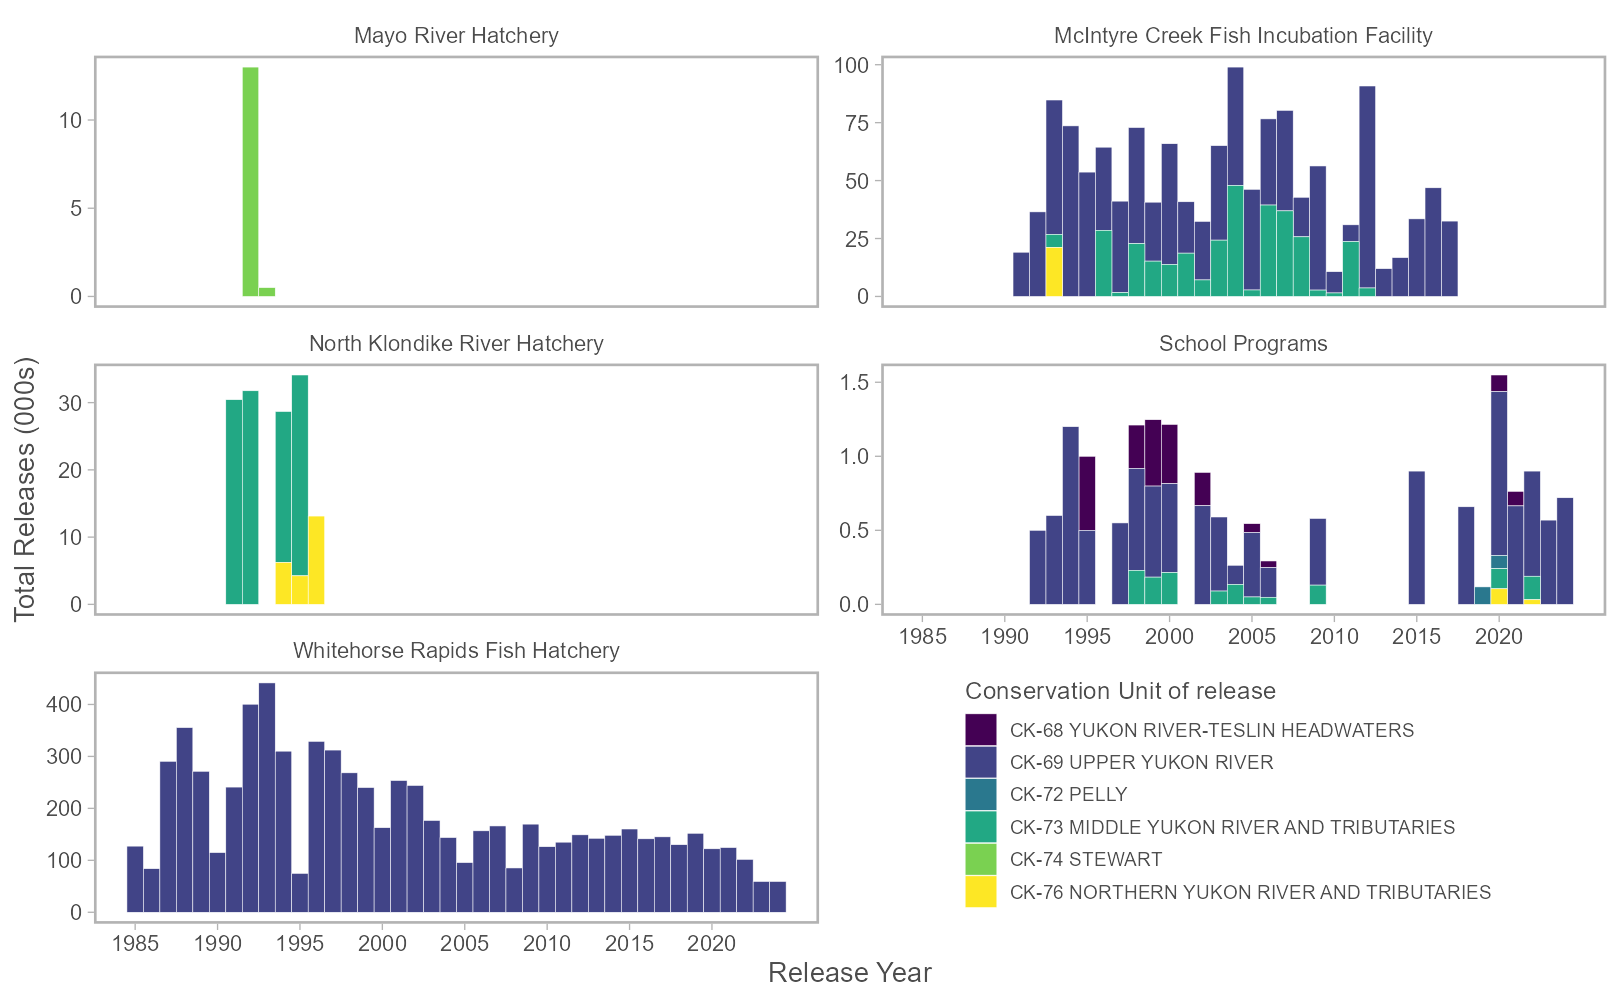
\includegraphics[width=6in]{figure/hatch_bar}}{Figure \ref{fig:fig-enhance-proj}} 

}

\caption{(ref:fig-enhance-proj)}\label{fig:fig-enhance-proj}
\end{figure}
(ref: fig-wh-fishway) Chinook returns to Whitehorse Rapids Fishway and proportion hatchery origin spawners (pHOS), based on observed adipose fin clip rates. Proportionate Natural Influence (PNI) for the last six years, calculated from adipose fin clip status and PBT results of broodstock, when available. PNI average (2019-2024) is 0.72.\,
\begin{figure}[htb]

{\centering \pdftooltip{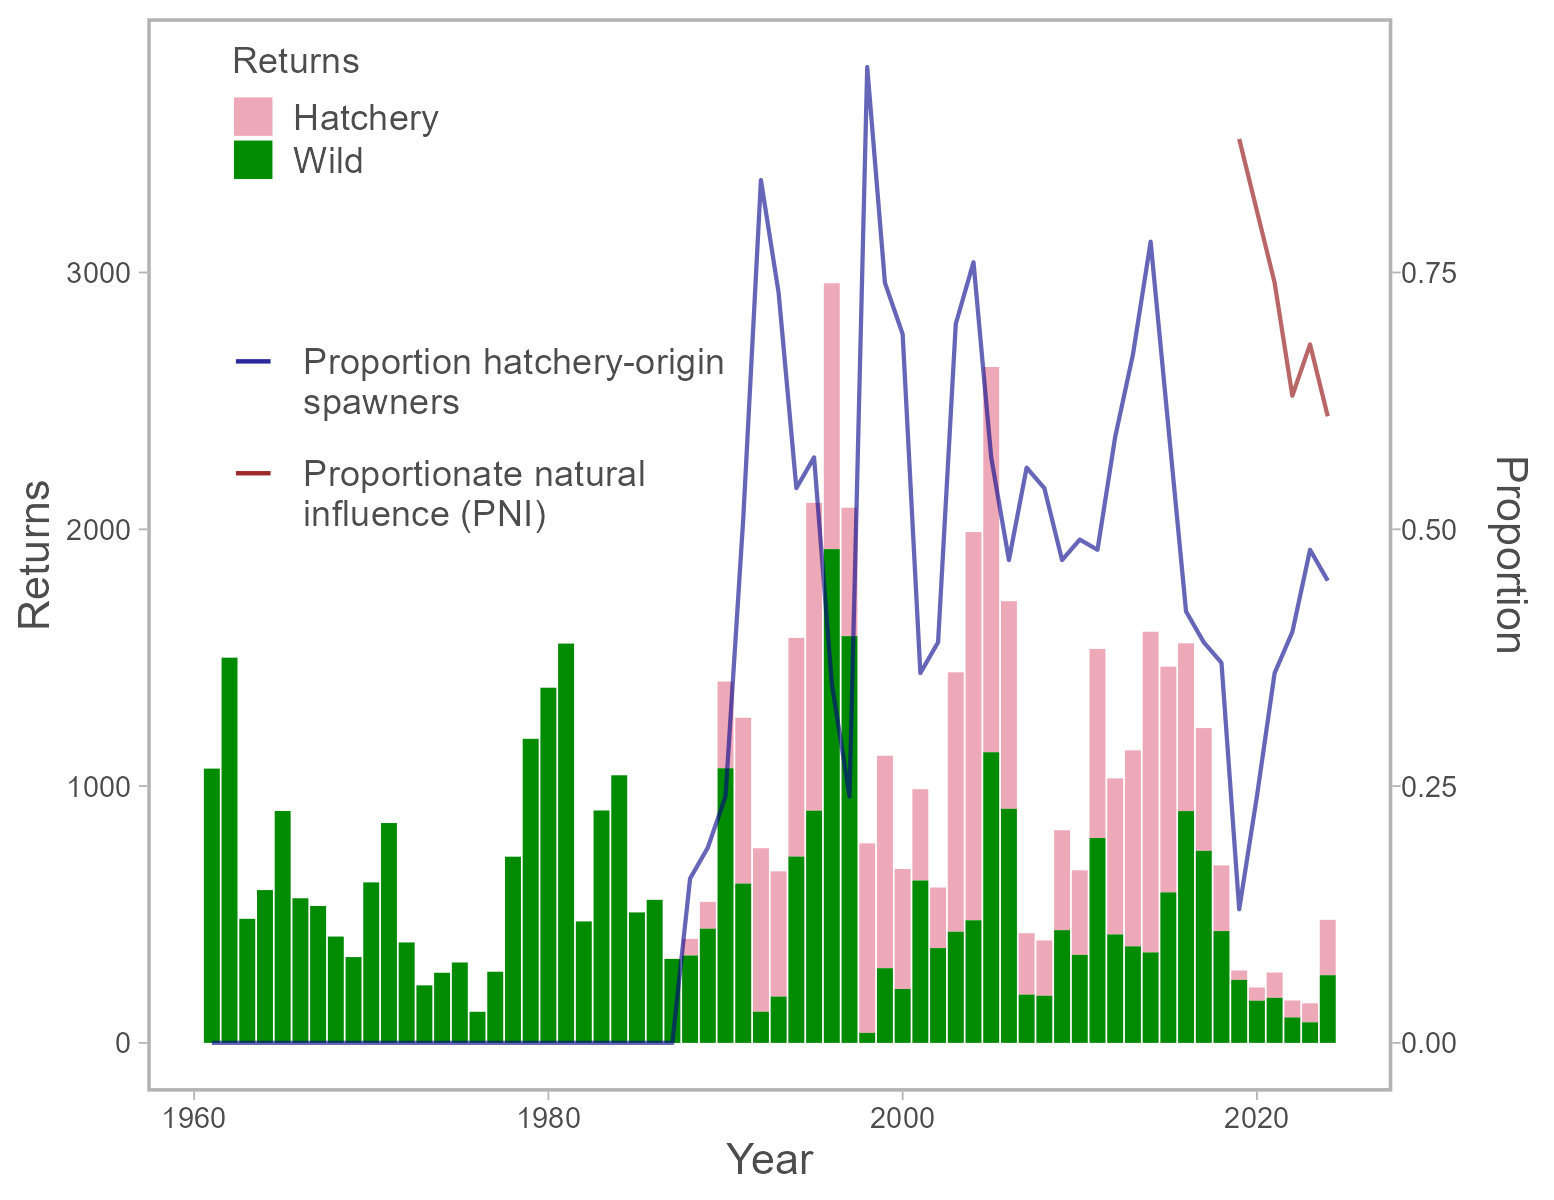
\includegraphics[width=6in]{figure/hatch_prop}}{Figure \ref{fig:fig-wh-fishway}} 

}

\caption{(ref:fig-wh-fishway)}\label{fig:fig-wh-fishway}
\end{figure}
\clearpage

\hypertarget{tables}{%
\section{TABLES}\label{tables}}


\begin{longtable}[t]{>{\raggedright\arraybackslash}p{3cm}>{\raggedright\arraybackslash}p{2cm}>{\raggedright\arraybackslash}p{4cm}>{\raggedright\arraybackslash}p{2cm}} \caption{\label{tab:tab-cons-unit-smu}Stock management units for Canadian Yukon River Chinook (CK) salmon and their component conservation units, with CU contribution from 1985-2024.}\\ \toprule Stock Management Unit & Conservation Unit Indicator & Conservation Unit Name & Average Contribution (1984-2024)\\ \midrule \endfirsthead \multicolumn{4}{l}{\textit{... Continued from previous page}} \\ \hline \caption*{}\\ \toprule Stock Management Unit & Conservation Unit Indicator & Conservation Unit Name & Average Contribution (1984-2024)\\ \midrule \endhead \hline \multicolumn{4}{l}{\textit{Continued on next page ...}} \\ \endfoot \bottomrule \endlastfoot YUKON CHINOOK SALMON & CK-68 & Yukon River-Teslin headwaters & 10.77\%\\  & CK-69 & Upper Yukon River & 4.76\%\\  & CK-70 & Big Salmon & N/A\\  & CK-71 & Nordenskiold & 1.27\%\\  & CK-72 & Pelly & 18.27\%\\  & CK-73 & Middle Yukon River and tributaries & 42.98\%\\  & CK-74 & Stewart & 6.14\%\\  & CK-75 & White and tributaries & 6.05\%\\  & CK-76 & North Yukon River and tributaries & 11.45\%\\ PORCUPINE CHINOOK SALMON & CK-77 & Salmon Fork & N/A\\  & CK-78 & Porcupine & N/A\\  & CK-79 & Old Crow & N/A\\* \end{longtable}

\clearpage


\begin{longtable}[t]{l>{\raggedright\arraybackslash}p{1.5cm}>{\raggedright\arraybackslash}p{1.5cm}>{\raggedright\arraybackslash}p{1.5cm}>{\raggedright\arraybackslash}p{1.5cm}>{\raggedright\arraybackslash}p{1.5cm}>{\raggedright\arraybackslash}p{1.5cm}>{\raggedright\arraybackslash}p{1.5cm}>{\raggedright\arraybackslash}p{1.5cm}} \caption{\label{tab:tab-CU-gsi-annual-summary}Annual proportion of conservation unit contribution, based on raw genetic stock identification assignments. Note that this accounts for GSI assignment uncertainty (i.e., sums across all probabilities and the re-scales by sample size for a given year) but is unweighted by border passage (i.e., does not account for incomplete sampling of return migration).}\\ \toprule Year & Middle Yukon River & North Yukon River & Nordenskiold & Pelly & Stewart & Teslin & Upper Yukon River & White\\ \midrule \endfirsthead \multicolumn{9}{l}{\textit{... Continued from previous page}} \\ \hline \caption*{}\\ \toprule Year & Middle Yukon River & North Yukon River & Nordenskiold & Pelly & Stewart & Teslin & Upper Yukon River & White\\ \midrule \endhead \hline \multicolumn{9}{l}{\textit{Continued on next page ...}} \\ \endfoot \bottomrule \endlastfoot 1985 & 0.298 & 0.05 & 0.02 & 0.191 & 0.136 & 0.205 & 0.043 & 0.055\\ 1986 & 0.262 & 0.094 & 0.009 & 0.207 & 0.1 & 0.196 & 0.041 & 0.088\\ 1987 & 0.322 & 0.112 & 0.007 & 0.293 & 0.073 & 0.096 & 0.022 & 0.073\\ 1991 & 0.417 & 0.124 & 0 & 0.206 & 0.08 & 0.103 & 0.058 & 0.011\\ 1992 & 0.178 & 0.192 & 0 & 0.246 & 0.049 & 0.23 & 0.016 & 0.088\\ 1993 & 0.247 & 0.224 & 0.004 & 0.149 & 0.025 & 0.161 & 0.027 & 0.167\\ 1994 & 0.286 & 0.221 & 0.013 & 0.172 & 0.085 & 0.077 & 0.044 & 0.101\\ 1995 & 0.424 & 0.113 & 0.023 & 0.12 & 0.104 & 0.108 & 0.052 & 0.054\\ 1996 & 0.358 & 0.077 & 0.016 & 0.138 & 0.053 & 0.169 & 0.048 & 0.14\\ 1997 & 0.479 & 0.092 & 0.007 & 0.131 & 0.071 & 0.091 & 0.076 & 0.052\\ 1999 & 0.332 & 0.112 & 0.017 & 0.158 & 0.057 & 0.155 & 0.074 & 0.093\\ 2000 & 0.405 & 0.076 & 0.042 & 0.186 & 0.046 & 0.101 & 0.049 & 0.093\\ 2001 & 0.116 & 0.308 & 0.009 & 0.246 & 0.081 & 0.077 & 0 & 0.162\\ 2002 & 0.568 & 0.136 & 0.013 & 0.117 & 0.079 & 0.026 & 0.038 & 0.022\\ 2003 & 0.376 & 0.207 & 0 & 0.258 & 0.031 & 0.05 & 0.02 & 0.061\\ 2004 & 0.328 & 0.215 & 0.006 & 0.215 & 0.062 & 0.072 & 0.044 & 0.056\\ 2005 & 0.353 & 0.172 & 0.003 & 0.186 & 0.031 & 0.147 & 0.033 & 0.074\\ 2006 & 0.542 & 0.121 & 0 & 0.142 & 0.069 & 0.042 & 0.05 & 0.034\\ 2007 & 0.207 & 0.173 & 0.015 & 0.274 & 0.091 & 0.12 & 0.011 & 0.109\\ 2008 & 0.607 & 0.182 & 0.029 & 0.249 & 0.103 & 0.06 & 0.016 & 0.077\\ 2009 & 0.338 & 0.12 & 0.018 & 0.262 & 0.083 & 0.094 & 0.029 & 0.055\\ 2010 & 0.323 & 0.083 & 0.016 & 0.328 & 0.046 & 0.125 & 0.05 & 0.029\\ 2011 & 0.509 & 0.102 & 0.022 & 0.309 & 0.062 & 0.175 & 0.063 & 0.054\\ 2012 & 0.232 & 0.179 & 0.016 & 0.247 & 0.023 & 0.139 & 0.052 & 0.111\\ 2013 & 0.62 & 0.01 & 0 & 0.172 & 0.046 & 0.08 & 0.069 & 0.003\\ 2014 & 0.562 & 0.049 & 0.018 & 0.168 & 0.052 & 0.066 & 0.04 & 0.044\\ 2015 & 0.497 & 0.062 & 0.017 & 0.187 & 0.066 & 0.076 & 0.046 & 0.048\\ 2016 & 0.478 & 0.054 & 0.007 & 0.154 & 0.066 & 0.151 & 0.064 & 0.024\\ 2017 & 0.55 & 0.061 & 0.017 & 0.123 & 0.044 & 0.125 & 0.051 & 0.03\\ 2018 & 0.601 & 0.053 & 0.013 & 0.085 & 0.046 & 0.086 & 0.087 & 0.029\\ 2019 & 0.63 & 0.033 & 0.01 & 0.12 & 0.041 & 0.079 & 0.059 & 0.029\\ 2020 & 0.546 & 0.068 & 0.009 & 0.177 & 0.055 & 0.096 & 0.03 & 0.02\\ 2021 & 0.533 & 0.07 & 0.028 & 0.13 & 0.083 & 0.077 & 0.051 & 0.03\\ 2022 & 0.705 & 0.065 & 0 & 0.097 & 0.006 & 0.038 & 0.077 & 0.011\\ 2023 & 0.594 & 0.074 & 0.03 & 0.066 & 0.02 & 0.114 & 0.065 & 0.036\\ 2024 & 0.651 & 0.037 & 0 & 0.068 & 0.044 & 0.07 & 0.117 & 0.013\\* \end{longtable}

\clearpage


\begin{longtable}[t]{>{\raggedright\arraybackslash}p{2cm}>{\raggedright\arraybackslash}p{3cm}>{\raggedright\arraybackslash}p{6.5cm}>{\raggedright\arraybackslash}p{5cm}} \caption{\label{tab:tab-factors-summary}Summary of anthropogenic, ecosystem, and climate factors affecting the stock.}\\ \toprule Life stage & Anthropogenic, ecosystem, or climate factor & Description or hypothesis & References\\ \midrule \endfirsthead \multicolumn{4}{l}{\textit{... Continued from previous page}} \\ \hline \caption*{}\\ \toprule Life stage & Anthropogenic, ecosystem, or climate factor & Description or hypothesis & References\\ \midrule \endhead \hline \multicolumn{4}{l}{\textit{Continued on next page ...}} \\ \endfoot \bottomrule \endlastfoot Spawner & Water temperature & Temperatures >18C cause heat stress and impact spawning success & Feddern et al. 2024; Murdoch et al. 2024\\ Spawner & Discharge/flow levels & Low flow reduce spawning success via higher temperature, habitat fragmentation & Howard and von Biela 2023; Neuswanger et al. 2015\\ Spawner & Ichthypohonus hoferi (pathogen) & Primarily infects maturing adults in the marine environment, potentially high mortality during spawning migration & Carroll and Liller 2023; Murphy et al. 2023; 2024; Kocan et al. 2004\\ Spawner & Thiamine deficiency complex (TDC) & Low thiamine in adults has transgenerational effects & Larson and Howard 2019; Howard and von Biela 2023\\ Egg & Stream flow & High flows scour streambeds, reducing egg survival & Feddern et al. 2024\\ Egg & Winter stream temperature & Cold and/or long winters reduce incubation survival & Murdoch et al. 2020; 2024\\ Fry / smolt & Aufeis (icing) & Reduced or halted streamflow from ice formations decreases fry survival & von Finster et al. 2025; in press\\ Fry / smolt & Stream flow / precipitation & High streamflow (high precipitation) may reduce foraging efficiency & Murdoch et al. 2024; Feddern et al. 2024\\ Fry / smolt & Ice out date & Early ice-out allows earlier outmigration & Murdoch et al. 2024; Cunningham et al. 2018; Feddern et al. 2024\\ Fry / smolt & Hydroelectric dam & Fry/smolts pass through dam, decreasing downstream survival & Twardek et al. 2023b\\ Fry / smolt & Placer mining & Sediment deposition and suspension can decrease egg and fry survival & Jensen et al. 2009; von Finster et al. in press\\ Juvenile & Sea surface temperature - winter & Colder first winters result in less productivity & Feddern et al. 2024\\ Juvenile & Sea ice cover & Productivity is lower in years when ice persists in the Bering Sea later & Feddern et al. 2024; Murdoch et al. 2024\\ Juvenile & Predation & Increase in apex predator abundance & Ohlberger et al. 2019\\ Adult & Pink salmon competition & Abundant pink salmon cause trophic cascades in the Bering Sea & Ruggerone et al. 2016; Cunningham et al. 2018\\ Adult & Prey quality & Declining prey quality in the Eastern Bering Sea hypothesized to be the cause of thiamine deficiency in spawning adults & Howard and von Biela 2023\\* \end{longtable}

\clearpage


\begin{longtable}[t]{l>{\raggedright\arraybackslash}p{6.5cm}c} \caption{\label{tab:tab-perf-metrics-descriptions}Biological and fishery performance measures used in the closed-loop simulations to assess HCR performance.}\\ \toprule Metric & Description & Equation\\ \midrule \endfirsthead \multicolumn{3}{l}{\textit{... Continued from previous page}} \\ \hline \caption*{}\\ \toprule Metric & Description & Equation\\ \midrule \endhead \hline \multicolumn{3}{l}{\textit{Continued on next page ...}} \\ \endfoot \bottomrule \endlastfoot \% replicate simulations < LRP & Probability the stock spawner abundance falls below the Limit Reference Point across replicate simulations and years, where $n$ rep is the number of replicate simulations and $t_1$ and $t_2$ are the first and last years over which the metric is calculated & $\frac{\sum_{\substack{n_{rep}\\s =1}}\sum_{\substack{t_1\\s   _2}}S_t<S_{gen}} {t_2-t_1+1}$\\ \% replicate simulations > USR & Probability the stock spawner abundance falls above the Upper Stock Reference Point across replicate simulations and years & $\frac{\sum_{\substack{n_{rep}\\s =1}}\sum_{\substack{t_1\\s  _2}}S_t>0.8S_{MSY}} {t_2-t_1+1}$\\ average annual catch & Average catch across replicate simulations and years & $\frac{\sum_{\substack{n_{rep}\\s =1}}\sum_{\substack{t_1\\s   _2}}S_tC_t} {t_2-t_1+1}$\\ catch stability (1/CV) & Stability in average catch across replicate simulations and years($\mu_C$), where is $\sigma_C$ the standard deviation in catch & $\cfrac{1}{\tfrac{\sigma_C}{\mu_C}}$\\ relative catch metric & Probability annual catch is greater than the average of the top 3 years of catch since 2000 ($C_{top}$), a semi-arbitrary indicator of a ‘good year’ & $\frac{\sum_{\substack{n_{rep}\\s =1}}\sum_{\substack{t_1\\s    _2}}C_t>C_{top}} {t_2-t_1+1}$\\* \end{longtable}

\clearpage


\begin{longtable}[t]{>{\raggedright\arraybackslash}p{3cm}>{\raggedright\arraybackslash}p{3cm}>{\raggedright\arraybackslash}p{10cm}} \caption{\label{tab:ref-points}Definitions of some common biological reference points used for salmon at either Stock Management Unit or Conservation Unit scale.}\\ \toprule Reference & Scale & Definition\\ \midrule \endfirsthead \multicolumn{3}{l}{\textit{... Continued from previous page}} \\ \hline \caption*{}\\ \toprule Reference & Scale & Definition\\ \midrule \endhead \hline \multicolumn{3}{l}{\textit{Continued on next page ...}} \\ \endfoot \bottomrule \endlastfoot Limit Reference Point (LRP) & Stock Management Unit & CU-status based, meaning that whether an SMU is above or below its LRP depends on whether any component CUs are below their lower biological benchmark (in the ‘red’ Wild Salmon Policy status zone). This definition is aligned with principle that LRPs be aligned with Canada’s WSP objective of preserving biodiversity of salmon at the scale of CUs. However, it is difficult to operationalize this type of LRP for fisheries management and so there may also be a “lower stock reference point” that is abundance based.\\ Upper Stock Reference Point (USR) & Stock Management Unit & Spawning abundance associated with fully meeting socio-economic objectives for the system, and above which maximum allowable harvest rates (see Removal Reference Point) can be sustained. Under the DFO Precautionary Approach Framework this is often 80\% of $S_{MSY}$, but this is not a requirement and may vary by system depending on the fishery and broader socio-economic and ecosystem objectives.\\ Removal Reference Point & Stock Management Unit or Conservation Unit & The maximum acceptable harvest rate the SMU can be subject to; is typically set to be less than or equal to the removal rate associated with maximum sustainable yield ($U_{MSY}$).\\ Lower stock reference point & Stock Management Unit & Aggregate SMU spawner abundance below which all fishery removals should be limited to the maximum extent possible and below which there is a high risk of serious and irreversible harm to the stock. This type of reference point is helpful for informing management since assessment and fishery decisions are often abundance based and so can be operationalized.\\ Lower Wild Salmon Policy biological benchmark & Conservation Unit & Differentiates amber and red Wild Salmon Policy status zones. When it can be estimated $S_{GEN}$ is often used and it is the spawning abundance that is expected to lead to recovery to $S_{MSY}$ in one salmon generation in the absence of fishing under equilibrium conditions. Spawning abundances below this reference point (red status) are expected to be associated with high risk of irreversible harm to the CU and align with a COSEWIC assessment of “endangered”.\\ Upper Wild Salmon Policy biological benchmark & Conservation Unit & The spawning abundance that differentiates amber and green Wild Salmon Policy status zones. When it can be estimated 80\%$S_{MSY}$ is used and is the spawner abundance expected to provide, on average annual basis, the maximum annual catch for the CU, given existing environmental conditions and where “there would not be a high probability of losing the CU”\\ Other biological reference points & Stock Management Unit or Conservation Unit & Other biologically based reference points like $S_{MSR}$, which is the spawner abundance expected to maximize returns on average annual basis, may be used as an upper biological reference point and 20\% of $S_{MSR}$ which has been proposed as a lower biological reference point. $S_{MSR}$ is sometimes referred to as $S_{MAX}$, and escapement goals based on this quantity are sometimes deemed more appropriate where the fishery is dominated by subsistence fisheries that wish to harvest a fixed number of fish each year and are attempting to minimize the effort needed to harvest.\\* \end{longtable}

\clearpage


\begin{longtable}[t]{llcllc} \caption{\label{tab:pars-ref-pts}Population (conservation unit) reference points. Values are in thousands of fish.}\\ \toprule Conservation Unit & Benchmark & Mean & Median & Quantile 10 & Quantile 90\\ \midrule \endfirsthead \multicolumn{6}{l}{\textit{... Continued from previous page}} \\ \hline \caption*{}\\ \toprule Conservation Unit & Benchmark & Mean & Median & Quantile 10 & Quantile 90\\ \midrule \endhead \hline \multicolumn{6}{l}{\textit{Continued on next page ...}} \\ \endfoot \bottomrule \endlastfoot  & Sgen & 1.47 & 1.42 & 0.76 & 2.19\\
\cmidrule{2-6}\nopagebreak  & Smsr & 9.1 & 8.47 & 6.25 & 12.56\\
\cmidrule{2-6}\nopagebreak  & Smsy & 3.81 & 3.62 & 1.65 & 5.99\\
\cmidrule{2-6}\nopagebreak \multirow{-4}{*}{\raggedright\arraybackslash Big Salmon} & Umsy & 0 & 0 & 0 & 0\\
\cmidrule{1-6}\pagebreak[0]  & Sgen & 2.5 & 2.42 & 1.41 & 3.63\\
\cmidrule{2-6}\nopagebreak  & Smsr & 15.4 & 14.59 & 11.23 & 20.44\\
\cmidrule{2-6}\nopagebreak  & Smsy & 7.66 & 7.48 & 4.77 & 10.58\\
\cmidrule{2-6}\nopagebreak \multirow{-4}{*}{\raggedright\arraybackslash MiddleYukonR andtribs} & Umsy & 0 & 0 & 0 & 0\\
\cmidrule{1-6}\pagebreak[0]  & Sgen & 0.45 & 0.44 & 0.28 & 0.63\\
\cmidrule{2-6}\nopagebreak  & Smsr & 2.84 & 2.74 & 2.21 & 3.56\\
\cmidrule{2-6}\nopagebreak  & Smsy & 1.59 & 1.57 & 1.25 & 1.98\\
\cmidrule{2-6}\nopagebreak \multirow{-4}{*}{\raggedright\arraybackslash Nordenskiold} & Umsy & 0 & 0 & 0 & 0\\
\cmidrule{1-6}\pagebreak[0]  & Sgen & 5.08 & 2.47 & 1.2 & 5.21\\
\cmidrule{2-6}\nopagebreak  & Smsr & 39.32 & 15.09 & 9.34 & 33.26\\
\cmidrule{2-6}\nopagebreak  & Smsy & 9.11 & 5.15 & 2 & 11.05\\
\cmidrule{2-6}\nopagebreak \multirow{-4}{*}{\raggedright\arraybackslash NorthernYukonR andtribs} & Umsy & 0 & 0 & 0 & 0\\
\cmidrule{1-6}\pagebreak[0]  & Sgen & 2.09 & 2.07 & 1 & 3.06\\
\cmidrule{2-6}\nopagebreak  & Smsr & 13.47 & 12.57 & 9.8 & 17.76\\
\cmidrule{2-6}\nopagebreak  & Smsy & 5.04 & 4.81 & 1.64 & 8.46\\
\cmidrule{2-6}\nopagebreak \multirow{-4}{*}{\raggedright\arraybackslash Pelly} & Umsy & 0 & 0 & 0 & 0\\
\cmidrule{1-6}\pagebreak[0]  & Sgen & 0.8 & 0.75 & 0.43 & 1.2\\
\cmidrule{2-6}\nopagebreak  & Smsr & 4.87 & 4.46 & 3.26 & 6.82\\
\cmidrule{2-6}\nopagebreak  & Smsy & 2.28 & 2.15 & 1.35 & 3.31\\
\cmidrule{2-6}\nopagebreak \multirow{-4}{*}{\raggedright\arraybackslash Stewart} & Umsy & 0 & 0 & 0 & 0\\
\cmidrule{1-6}\pagebreak[0]  & Sgen & 1 & 0.98 & 0.5 & 1.5\\
\cmidrule{2-6}\nopagebreak  & Smsr & 6.66 & 6.3 & 4.88 & 8.68\\
\cmidrule{2-6}\nopagebreak  & Smsy & 3.41 & 3.32 & 1.6 & 5.16\\
\cmidrule{2-6}\nopagebreak \multirow{-4}{*}{\raggedright\arraybackslash UpperYukonR} & Umsy & 0 & 0 & 0 & 0\\
\cmidrule{1-6}\pagebreak[0]  & Sgen & 0.83 & 0.81 & 0.39 & 1.27\\
\cmidrule{2-6}\nopagebreak  & Smsr & 5.4 & 5.08 & 3.78 & 7.29\\
\cmidrule{2-6}\nopagebreak  & Smsy & 2.6 & 2.51 & 1.14 & 4.07\\
\cmidrule{2-6}\nopagebreak \multirow{-4}{*}{\raggedright\arraybackslash Whiteandtribs} & Umsy & 0 & 0 & 0 & 0\\
\cmidrule{1-6}\pagebreak[0]  & Sgen & 0.85 & 0.82 & 0.49 & 1.26\\
\cmidrule{2-6}\nopagebreak  & Smsr & 5.76 & 5.57 & 4.44 & 7.31\\
\cmidrule{2-6}\nopagebreak  & Smsy & 3.37 & 3.33 & 2.54 & 4.26\\
\cmidrule{2-6}\nopagebreak \multirow{-4}{*}{\raggedright\arraybackslash YukonR Teslinheadwaters} & Umsy & 0 & 0 & 0 & 0\\* \end{longtable}

\clearpage


\begin{longtable}[t]{>{\raggedright\arraybackslash}p{3cm}lcl>{\raggedright\arraybackslash}p{2cm}>{\centering\arraybackslash}p{2cm}>{\raggedright\arraybackslash}p{2cm}>{\raggedright\arraybackslash}p{2cm}} \caption{\label{tab:pars-sr}Population (conservation unit) reference points. Values are in thousands of fish.}\\ \toprule Conservation Unit & Parameter & Mean & Median & Quantile 10 & Quantile 90 & Effective Sample Size (Neff) & Chain Mixing (Rhat)\\ \midrule \endfirsthead \multicolumn{8}{l}{\textit{... Continued from previous page}} \\ \hline \caption*{}\\ \toprule Conservation Unit & Parameter & Mean & Median & Quantile 10 & Quantile 90 & Effective Sample Size (Neff) & Chain Mixing (Rhat)\\ \midrule \endhead \hline \multicolumn{8}{l}{\textit{Continued on next page ...}} \\ \endfoot \bottomrule \endlastfoot \multicolumn{1}{>{\centering\arraybackslash}p{3cm}}{} & \multicolumn{1}{c}{alpha} & \multicolumn{1}{c}{2.92} & \multicolumn{1}{c}{2.74} & \multicolumn{1}{>{\centering\arraybackslash}p{2cm}}{1.48} & \multicolumn{1}{>{\centering\arraybackslash}p{2cm}}{5.72} & \multicolumn{1}{>{\centering\arraybackslash}p{2cm}}{3595} & \multicolumn{1}{>{\centering\arraybackslash}p{2cm}}{1}\\
\cmidrule{2-8}\nopagebreak \multicolumn{1}{>{\centering\arraybackslash}p{3cm}}{} & \multicolumn{1}{c}{beta} & \multicolumn{1}{c}{0} & \multicolumn{1}{c}{0} & \multicolumn{1}{>{\centering\arraybackslash}p{2cm}}{0} & \multicolumn{1}{>{\centering\arraybackslash}p{2cm}}{0} & \multicolumn{1}{>{\centering\arraybackslash}p{2cm}}{5626} & \multicolumn{1}{>{\centering\arraybackslash}p{2cm}}{1}\\
\cmidrule{2-8}\nopagebreak \multicolumn{1}{>{\centering\arraybackslash}p{3cm}}{} & \multicolumn{1}{c}{phi} & \multicolumn{1}{c}{0.82} & \multicolumn{1}{c}{0.84} & \multicolumn{1}{>{\centering\arraybackslash}p{2cm}}{0.67} & \multicolumn{1}{>{\centering\arraybackslash}p{2cm}}{0.96} & \multicolumn{1}{>{\centering\arraybackslash}p{2cm}}{4846} & \multicolumn{1}{>{\centering\arraybackslash}p{2cm}}{1}\\
\cmidrule{2-8}\nopagebreak \multicolumn{1}{>{\centering\arraybackslash}p{3cm}}{\multirow{-4}{*}{\raggedright\arraybackslash Big Salmon}} & \multicolumn{1}{c}{sigma} & \multicolumn{1}{c}{0.96} & \multicolumn{1}{c}{0.95} & \multicolumn{1}{>{\centering\arraybackslash}p{2cm}}{0.86} & \multicolumn{1}{>{\centering\arraybackslash}p{2cm}}{1.06} & \multicolumn{1}{>{\centering\arraybackslash}p{2cm}}{5761} & \multicolumn{1}{>{\centering\arraybackslash}p{2cm}}{1}\\
\cmidrule{1-8}\pagebreak[0] \multicolumn{1}{>{\centering\arraybackslash}p{3cm}}{} & \multicolumn{1}{c}{alpha} & \multicolumn{1}{c}{3.64} & \multicolumn{1}{c}{3.63} & \multicolumn{1}{>{\centering\arraybackslash}p{2cm}}{1.95} & \multicolumn{1}{>{\centering\arraybackslash}p{2cm}}{6.28} & \multicolumn{1}{>{\centering\arraybackslash}p{2cm}}{4272} & \multicolumn{1}{>{\centering\arraybackslash}p{2cm}}{1}\\
\cmidrule{2-8}\nopagebreak \multicolumn{1}{>{\centering\arraybackslash}p{3cm}}{} & \multicolumn{1}{c}{beta} & \multicolumn{1}{c}{0} & \multicolumn{1}{c}{0} & \multicolumn{1}{>{\centering\arraybackslash}p{2cm}}{0} & \multicolumn{1}{>{\centering\arraybackslash}p{2cm}}{0} & \multicolumn{1}{>{\centering\arraybackslash}p{2cm}}{5749} & \multicolumn{1}{>{\centering\arraybackslash}p{2cm}}{1}\\
\cmidrule{2-8}\nopagebreak \multicolumn{1}{>{\centering\arraybackslash}p{3cm}}{} & \multicolumn{1}{c}{phi} & \multicolumn{1}{c}{0.72} & \multicolumn{1}{c}{0.74} & \multicolumn{1}{>{\centering\arraybackslash}p{2cm}}{0.51} & \multicolumn{1}{>{\centering\arraybackslash}p{2cm}}{0.92} & \multicolumn{1}{>{\centering\arraybackslash}p{2cm}}{3919} & \multicolumn{1}{>{\centering\arraybackslash}p{2cm}}{1}\\
\cmidrule{2-8}\nopagebreak \multicolumn{1}{>{\centering\arraybackslash}p{3cm}}{\multirow{-4}{*}{\raggedright\arraybackslash MiddleYukonR andtribs}} & \multicolumn{1}{c}{sigma} & \multicolumn{1}{c}{1.02} & \multicolumn{1}{c}{1.02} & \multicolumn{1}{>{\centering\arraybackslash}p{2cm}}{0.92} & \multicolumn{1}{>{\centering\arraybackslash}p{2cm}}{1.12} & \multicolumn{1}{>{\centering\arraybackslash}p{2cm}}{6255} & \multicolumn{1}{>{\centering\arraybackslash}p{2cm}}{1}\\
\cmidrule{1-8}\pagebreak[0] \multicolumn{1}{>{\centering\arraybackslash}p{3cm}}{} & \multicolumn{1}{c}{alpha} & \multicolumn{1}{c}{4.23} & \multicolumn{1}{c}{4.24} & \multicolumn{1}{>{\centering\arraybackslash}p{2cm}}{2.79} & \multicolumn{1}{>{\centering\arraybackslash}p{2cm}}{6.32} & \multicolumn{1}{>{\centering\arraybackslash}p{2cm}}{3762} & \multicolumn{1}{>{\centering\arraybackslash}p{2cm}}{1}\\
\cmidrule{2-8}\nopagebreak \multicolumn{1}{>{\centering\arraybackslash}p{3cm}}{} & \multicolumn{1}{c}{beta} & \multicolumn{1}{c}{0} & \multicolumn{1}{c}{0} & \multicolumn{1}{>{\centering\arraybackslash}p{2cm}}{0} & \multicolumn{1}{>{\centering\arraybackslash}p{2cm}}{0} & \multicolumn{1}{>{\centering\arraybackslash}p{2cm}}{9173} & \multicolumn{1}{>{\centering\arraybackslash}p{2cm}}{1}\\
\cmidrule{2-8}\nopagebreak \multicolumn{1}{>{\centering\arraybackslash}p{3cm}}{} & \multicolumn{1}{c}{phi} & \multicolumn{1}{c}{0.54} & \multicolumn{1}{c}{0.54} & \multicolumn{1}{>{\centering\arraybackslash}p{2cm}}{0.27} & \multicolumn{1}{>{\centering\arraybackslash}p{2cm}}{0.79} & \multicolumn{1}{>{\centering\arraybackslash}p{2cm}}{3177} & \multicolumn{1}{>{\centering\arraybackslash}p{2cm}}{1}\\
\cmidrule{2-8}\nopagebreak \multicolumn{1}{>{\centering\arraybackslash}p{3cm}}{\multirow{-4}{*}{\raggedright\arraybackslash Nordenskiold}} & \multicolumn{1}{c}{sigma} & \multicolumn{1}{c}{1.11} & \multicolumn{1}{c}{1.1} & \multicolumn{1}{>{\centering\arraybackslash}p{2cm}}{1} & \multicolumn{1}{>{\centering\arraybackslash}p{2cm}}{1.22} & \multicolumn{1}{>{\centering\arraybackslash}p{2cm}}{6902} & \multicolumn{1}{>{\centering\arraybackslash}p{2cm}}{1}\\
\cmidrule{1-8}\pagebreak[0] \multicolumn{1}{>{\centering\arraybackslash}p{3cm}}{} & \multicolumn{1}{c}{alpha} & \multicolumn{1}{c}{2.33} & \multicolumn{1}{c}{2.14} & \multicolumn{1}{>{\centering\arraybackslash}p{2cm}}{1.27} & \multicolumn{1}{>{\centering\arraybackslash}p{2cm}}{4.33} & \multicolumn{1}{>{\centering\arraybackslash}p{2cm}}{4377} & \multicolumn{1}{>{\centering\arraybackslash}p{2cm}}{1}\\
\cmidrule{2-8}\nopagebreak \multicolumn{1}{>{\centering\arraybackslash}p{3cm}}{} & \multicolumn{1}{c}{beta} & \multicolumn{1}{c}{0} & \multicolumn{1}{c}{0} & \multicolumn{1}{>{\centering\arraybackslash}p{2cm}}{0} & \multicolumn{1}{>{\centering\arraybackslash}p{2cm}}{0} & \multicolumn{1}{>{\centering\arraybackslash}p{2cm}}{5880} & \multicolumn{1}{>{\centering\arraybackslash}p{2cm}}{1}\\
\cmidrule{2-8}\nopagebreak \multicolumn{1}{>{\centering\arraybackslash}p{3cm}}{} & \multicolumn{1}{c}{phi} & \multicolumn{1}{c}{0.8} & \multicolumn{1}{c}{0.8} & \multicolumn{1}{>{\centering\arraybackslash}p{2cm}}{0.66} & \multicolumn{1}{>{\centering\arraybackslash}p{2cm}}{0.93} & \multicolumn{1}{>{\centering\arraybackslash}p{2cm}}{5643} & \multicolumn{1}{>{\centering\arraybackslash}p{2cm}}{1}\\
\cmidrule{2-8}\nopagebreak \multicolumn{1}{>{\centering\arraybackslash}p{3cm}}{\multirow{-4}{*}{\raggedright\arraybackslash NorthernYukonR andtribs}} & \multicolumn{1}{c}{sigma} & \multicolumn{1}{c}{1.02} & \multicolumn{1}{c}{1.02} & \multicolumn{1}{>{\centering\arraybackslash}p{2cm}}{0.92} & \multicolumn{1}{>{\centering\arraybackslash}p{2cm}}{1.13} & \multicolumn{1}{>{\centering\arraybackslash}p{2cm}}{7048} & \multicolumn{1}{>{\centering\arraybackslash}p{2cm}}{1}\\
\cmidrule{1-8}\pagebreak[0] \multicolumn{1}{>{\centering\arraybackslash}p{3cm}}{} & \multicolumn{1}{c}{alpha} & \multicolumn{1}{c}{2.59} & \multicolumn{1}{c}{2.35} & \multicolumn{1}{>{\centering\arraybackslash}p{2cm}}{1.3} & \multicolumn{1}{>{\centering\arraybackslash}p{2cm}}{5.3} & \multicolumn{1}{>{\centering\arraybackslash}p{2cm}}{3235} & \multicolumn{1}{>{\centering\arraybackslash}p{2cm}}{1}\\
\cmidrule{2-8}\nopagebreak \multicolumn{1}{>{\centering\arraybackslash}p{3cm}}{} & \multicolumn{1}{c}{beta} & \multicolumn{1}{c}{0} & \multicolumn{1}{c}{0} & \multicolumn{1}{>{\centering\arraybackslash}p{2cm}}{0} & \multicolumn{1}{>{\centering\arraybackslash}p{2cm}}{0} & \multicolumn{1}{>{\centering\arraybackslash}p{2cm}}{5755} & \multicolumn{1}{>{\centering\arraybackslash}p{2cm}}{1}\\
\cmidrule{2-8}\nopagebreak \multicolumn{1}{>{\centering\arraybackslash}p{3cm}}{} & \multicolumn{1}{c}{phi} & \multicolumn{1}{c}{0.85} & \multicolumn{1}{c}{0.86} & \multicolumn{1}{>{\centering\arraybackslash}p{2cm}}{0.72} & \multicolumn{1}{>{\centering\arraybackslash}p{2cm}}{0.97} & \multicolumn{1}{>{\centering\arraybackslash}p{2cm}}{4872} & \multicolumn{1}{>{\centering\arraybackslash}p{2cm}}{1}\\
\cmidrule{2-8}\nopagebreak \multicolumn{1}{>{\centering\arraybackslash}p{3cm}}{\multirow{-4}{*}{\raggedright\arraybackslash Pelly}} & \multicolumn{1}{c}{sigma} & \multicolumn{1}{c}{0.96} & \multicolumn{1}{c}{0.96} & \multicolumn{1}{>{\centering\arraybackslash}p{2cm}}{0.87} & \multicolumn{1}{>{\centering\arraybackslash}p{2cm}}{1.06} & \multicolumn{1}{>{\centering\arraybackslash}p{2cm}}{5838} & \multicolumn{1}{>{\centering\arraybackslash}p{2cm}}{1}\\
\cmidrule{1-8}\pagebreak[0] \multicolumn{1}{>{\centering\arraybackslash}p{3cm}}{} & \multicolumn{1}{c}{alpha} & \multicolumn{1}{c}{3.37} & \multicolumn{1}{c}{3.29} & \multicolumn{1}{>{\centering\arraybackslash}p{2cm}}{1.82} & \multicolumn{1}{>{\centering\arraybackslash}p{2cm}}{5.94} & \multicolumn{1}{>{\centering\arraybackslash}p{2cm}}{4116} & \multicolumn{1}{>{\centering\arraybackslash}p{2cm}}{1}\\
\cmidrule{2-8}\nopagebreak \multicolumn{1}{>{\centering\arraybackslash}p{3cm}}{} & \multicolumn{1}{c}{beta} & \multicolumn{1}{c}{0} & \multicolumn{1}{c}{0} & \multicolumn{1}{>{\centering\arraybackslash}p{2cm}}{0} & \multicolumn{1}{>{\centering\arraybackslash}p{2cm}}{0} & \multicolumn{1}{>{\centering\arraybackslash}p{2cm}}{6048} & \multicolumn{1}{>{\centering\arraybackslash}p{2cm}}{1}\\
\cmidrule{2-8}\nopagebreak \multicolumn{1}{>{\centering\arraybackslash}p{3cm}}{} & \multicolumn{1}{c}{phi} & \multicolumn{1}{c}{0.69} & \multicolumn{1}{c}{0.7} & \multicolumn{1}{>{\centering\arraybackslash}p{2cm}}{0.48} & \multicolumn{1}{>{\centering\arraybackslash}p{2cm}}{0.89} & \multicolumn{1}{>{\centering\arraybackslash}p{2cm}}{4648} & \multicolumn{1}{>{\centering\arraybackslash}p{2cm}}{1}\\
\cmidrule{2-8}\nopagebreak \multicolumn{1}{>{\centering\arraybackslash}p{3cm}}{\multirow{-4}{*}{\raggedright\arraybackslash Stewart}} & \multicolumn{1}{c}{sigma} & \multicolumn{1}{c}{1.11} & \multicolumn{1}{c}{1.11} & \multicolumn{1}{>{\centering\arraybackslash}p{2cm}}{1.01} & \multicolumn{1}{>{\centering\arraybackslash}p{2cm}}{1.22} & \multicolumn{1}{>{\centering\arraybackslash}p{2cm}}{8050} & \multicolumn{1}{>{\centering\arraybackslash}p{2cm}}{1}\\
\cmidrule{1-8}\pagebreak[0] \multicolumn{1}{>{\centering\arraybackslash}p{3cm}}{} & \multicolumn{1}{c}{alpha} & \multicolumn{1}{c}{3.89} & \multicolumn{1}{c}{3.73} & \multicolumn{1}{>{\centering\arraybackslash}p{2cm}}{1.71} & \multicolumn{1}{>{\centering\arraybackslash}p{2cm}}{8.46} & \multicolumn{1}{>{\centering\arraybackslash}p{2cm}}{4123} & \multicolumn{1}{>{\centering\arraybackslash}p{2cm}}{1}\\
\cmidrule{2-8}\nopagebreak \multicolumn{1}{>{\centering\arraybackslash}p{3cm}}{} & \multicolumn{1}{c}{beta} & \multicolumn{1}{c}{0} & \multicolumn{1}{c}{0} & \multicolumn{1}{>{\centering\arraybackslash}p{2cm}}{0} & \multicolumn{1}{>{\centering\arraybackslash}p{2cm}}{0} & \multicolumn{1}{>{\centering\arraybackslash}p{2cm}}{7377} & \multicolumn{1}{>{\centering\arraybackslash}p{2cm}}{1}\\
\cmidrule{2-8}\nopagebreak \multicolumn{1}{>{\centering\arraybackslash}p{3cm}}{} & \multicolumn{1}{c}{phi} & \multicolumn{1}{c}{0.81} & \multicolumn{1}{c}{0.82} & \multicolumn{1}{>{\centering\arraybackslash}p{2cm}}{0.66} & \multicolumn{1}{>{\centering\arraybackslash}p{2cm}}{0.95} & \multicolumn{1}{>{\centering\arraybackslash}p{2cm}}{5355} & \multicolumn{1}{>{\centering\arraybackslash}p{2cm}}{1}\\
\cmidrule{2-8}\nopagebreak \multicolumn{1}{>{\centering\arraybackslash}p{3cm}}{\multirow{-4}{*}{\raggedright\arraybackslash UpperYukonR}} & \multicolumn{1}{c}{sigma} & \multicolumn{1}{c}{1.12} & \multicolumn{1}{c}{1.11} & \multicolumn{1}{>{\centering\arraybackslash}p{2cm}}{1.02} & \multicolumn{1}{>{\centering\arraybackslash}p{2cm}}{1.22} & \multicolumn{1}{>{\centering\arraybackslash}p{2cm}}{6667} & \multicolumn{1}{>{\centering\arraybackslash}p{2cm}}{1}\\
\cmidrule{1-8}\pagebreak[0] \multicolumn{1}{>{\centering\arraybackslash}p{3cm}}{} & \multicolumn{1}{c}{alpha} & \multicolumn{1}{c}{3.6} & \multicolumn{1}{c}{3.36} & \multicolumn{1}{>{\centering\arraybackslash}p{2cm}}{1.58} & \multicolumn{1}{>{\centering\arraybackslash}p{2cm}}{8.23} & \multicolumn{1}{>{\centering\arraybackslash}p{2cm}}{3273} & \multicolumn{1}{>{\centering\arraybackslash}p{2cm}}{1}\\
\cmidrule{2-8}\nopagebreak \multicolumn{1}{>{\centering\arraybackslash}p{3cm}}{} & \multicolumn{1}{c}{beta} & \multicolumn{1}{c}{0} & \multicolumn{1}{c}{0} & \multicolumn{1}{>{\centering\arraybackslash}p{2cm}}{0} & \multicolumn{1}{>{\centering\arraybackslash}p{2cm}}{0} & \multicolumn{1}{>{\centering\arraybackslash}p{2cm}}{5174} & \multicolumn{1}{>{\centering\arraybackslash}p{2cm}}{1}\\
\cmidrule{2-8}\nopagebreak \multicolumn{1}{>{\centering\arraybackslash}p{3cm}}{} & \multicolumn{1}{c}{phi} & \multicolumn{1}{c}{0.85} & \multicolumn{1}{c}{0.87} & \multicolumn{1}{>{\centering\arraybackslash}p{2cm}}{0.71} & \multicolumn{1}{>{\centering\arraybackslash}p{2cm}}{0.97} & \multicolumn{1}{>{\centering\arraybackslash}p{2cm}}{4795} & \multicolumn{1}{>{\centering\arraybackslash}p{2cm}}{1}\\
\cmidrule{2-8}\nopagebreak \multicolumn{1}{>{\centering\arraybackslash}p{3cm}}{\multirow{-4}{*}{\raggedright\arraybackslash Whiteandtribs}} & \multicolumn{1}{c}{sigma} & \multicolumn{1}{c}{0.97} & \multicolumn{1}{c}{0.96} & \multicolumn{1}{>{\centering\arraybackslash}p{2cm}}{0.86} & \multicolumn{1}{>{\centering\arraybackslash}p{2cm}}{1.08} & \multicolumn{1}{>{\centering\arraybackslash}p{2cm}}{4204} & \multicolumn{1}{>{\centering\arraybackslash}p{2cm}}{1}\\
\cmidrule{1-8}\pagebreak[0] \multicolumn{1}{>{\centering\arraybackslash}p{3cm}}{} & \multicolumn{1}{c}{alpha} & \multicolumn{1}{c}{4.71} & \multicolumn{1}{c}{4.78} & \multicolumn{1}{>{\centering\arraybackslash}p{2cm}}{2.78} & \multicolumn{1}{>{\centering\arraybackslash}p{2cm}}{7.67} & \multicolumn{1}{>{\centering\arraybackslash}p{2cm}}{3615} & \multicolumn{1}{>{\centering\arraybackslash}p{2cm}}{1}\\
\cmidrule{2-8}\nopagebreak \multicolumn{1}{>{\centering\arraybackslash}p{3cm}}{} & \multicolumn{1}{c}{beta} & \multicolumn{1}{c}{0} & \multicolumn{1}{c}{0} & \multicolumn{1}{>{\centering\arraybackslash}p{2cm}}{0} & \multicolumn{1}{>{\centering\arraybackslash}p{2cm}}{0} & \multicolumn{1}{>{\centering\arraybackslash}p{2cm}}{6974} & \multicolumn{1}{>{\centering\arraybackslash}p{2cm}}{1}\\
\cmidrule{2-8}\nopagebreak \multicolumn{1}{>{\centering\arraybackslash}p{3cm}}{} & \multicolumn{1}{c}{phi} & \multicolumn{1}{c}{0.64} & \multicolumn{1}{c}{0.65} & \multicolumn{1}{>{\centering\arraybackslash}p{2cm}}{0.41} & \multicolumn{1}{>{\centering\arraybackslash}p{2cm}}{0.86} & \multicolumn{1}{>{\centering\arraybackslash}p{2cm}}{2641} & \multicolumn{1}{>{\centering\arraybackslash}p{2cm}}{1}\\
\cmidrule{2-8}\nopagebreak \multicolumn{1}{>{\centering\arraybackslash}p{3cm}}{\multirow{-4}{*}{\raggedright\arraybackslash YukonR Teslinheadwaters}} & \multicolumn{1}{c}{sigma} & \multicolumn{1}{c}{1.07} & \multicolumn{1}{c}{1.07} & \multicolumn{1}{>{\centering\arraybackslash}p{2cm}}{0.97} & \multicolumn{1}{>{\centering\arraybackslash}p{2cm}}{1.18} & \multicolumn{1}{>{\centering\arraybackslash}p{2cm}}{7880} & \multicolumn{1}{>{\centering\arraybackslash}p{2cm}}{1}\\* \end{longtable}

\clearpage


\begin{longtable}[t]{llcllc} \caption{\label{tab:demo-ref-pts}Population (conservation unit) reference points from demographic (egg mass) models. Values are in thousands of fish.}\\ \toprule Conservation Unit & Period & Benchmark & Median & Lower Quantile & Upper Quantile\\ \midrule \endfirsthead \multicolumn{6}{l}{\textit{... Continued from previous page}} \\ \hline \caption*{}\\ \toprule Conservation Unit & Period & Benchmark & Median & Lower Quantile & Upper Quantile\\ \midrule \endhead \hline \multicolumn{6}{l}{\textit{Continued on next page ...}} \\ \endfoot \bottomrule \endlastfoot  & Average (all years) & Smsr & 5.28 & 1.57 & 8.4\\
\cmidrule{2-6}\nopagebreak  & Average (all years) & Smsy & 2.75 & 0.76 & 4.74\\
\cmidrule{2-6}\nopagebreak  & Early() & Smsr & 4.06 & 2 & 6.61\\
\cmidrule{2-6}\nopagebreak  & Early() & Smsy & 2.4 & 0.93 & 3.91\\
\cmidrule{2-6}\nopagebreak  & Recent() & Smsr & 6.05 & 1.22 & 9.59\\
\cmidrule{2-6}\nopagebreak \multirow{-6}{*}{\raggedright\arraybackslash Big Salmon} & Recent() & Smsy & 2.92 & 0.6 & 5.37\\
\cmidrule{1-6}\pagebreak[0]  & Average (all years) & Smsr & 17.28 & 3.72 & 30.02\\
\cmidrule{2-6}\nopagebreak  & Average (all years) & Smsy & 8.76 & 1.82 & 15.91\\
\cmidrule{2-6}\nopagebreak  & Early() & Smsr & 13.46 & 3.46 & 24.83\\
\cmidrule{2-6}\nopagebreak  & Early() & Smsy & 7.73 & 1.69 & 13.55\\
\cmidrule{2-6}\nopagebreak  & Recent() & Smsr & 19.31 & 3.46 & 32.79\\
\cmidrule{2-6}\nopagebreak \multirow{-6}{*}{\raggedright\arraybackslash MiddleYukonR andtribs} & Recent() & Smsy & 9.19 & 1.7 & 17.89\\
\cmidrule{1-6}\pagebreak[0]  & Average (all years) & Smsr & 4.1 & 1.45 & 7.34\\
\cmidrule{2-6}\nopagebreak  & Average (all years) & Smsy & 2.08 & 0.69 & 3.84\\
\cmidrule{2-6}\nopagebreak  & Early() & Smsr & 3.22 & 1.77 & 6\\
\cmidrule{2-6}\nopagebreak  & Early() & Smsy & 1.85 & 0.83 & 3.28\\
\cmidrule{2-6}\nopagebreak  & Recent() & Smsr & 4.57 & 1.08 & 8.14\\
\cmidrule{2-6}\nopagebreak \multirow{-6}{*}{\raggedright\arraybackslash Nordenskiold} & Recent() & Smsy & 2.16 & 0.53 & 4.23\\
\cmidrule{1-6}\pagebreak[0]  & Average (all years) & Smsr & 11.08 & 1.32 & 30.04\\
\cmidrule{2-6}\nopagebreak  & Average (all years) & Smsy & 5.24 & 0.65 & 14.74\\
\cmidrule{2-6}\nopagebreak  & Early() & Smsr & 9.85 & 1.77 & 30.04\\
\cmidrule{2-6}\nopagebreak  & Early() & Smsy & 5.01 & 0.87 & 14.55\\
\cmidrule{2-6}\nopagebreak  & Recent() & Smsr & 10.96 & 0.95 & 30.46\\
\cmidrule{2-6}\nopagebreak \multirow{-6}{*}{\raggedright\arraybackslash NorthernYukonR andtribs} & Recent() & Smsy & 5.07 & 0.47 & 15.46\\
\cmidrule{1-6}\pagebreak[0]  & Average (all years) & Smsr & 11.39 & 1.01 & 30.38\\
\cmidrule{2-6}\nopagebreak  & Average (all years) & Smsy & 5.39 & 0.5 & 15.87\\
\cmidrule{2-6}\nopagebreak  & Early() & Smsr & 9.62 & 1.43 & 30.58\\
\cmidrule{2-6}\nopagebreak  & Early() & Smsy & 5.01 & 0.7 & 14.89\\
\cmidrule{2-6}\nopagebreak  & Recent() & Smsr & 11.61 & 0.73 & 31.63\\
\cmidrule{2-6}\nopagebreak \multirow{-6}{*}{\raggedright\arraybackslash Pelly} & Recent() & Smsy & 5.33 & 0.36 & 16.72\\
\cmidrule{1-6}\pagebreak[0]  & Average (all years) & Smsr & 4.85 & 2.33 & 7.71\\
\cmidrule{2-6}\nopagebreak  & Average (all years) & Smsy & 2.59 & 1.09 & 4.2\\
\cmidrule{2-6}\nopagebreak  & Early() & Smsr & 3.69 & 2.34 & 5.91\\
\cmidrule{2-6}\nopagebreak  & Early() & Smsy & 2.25 & 1.12 & 3.55\\
\cmidrule{2-6}\nopagebreak  & Recent() & Smsr & 5.66 & 1.86 & 8.89\\
\cmidrule{2-6}\nopagebreak \multirow{-6}{*}{\raggedright\arraybackslash Stewart} & Recent() & Smsy & 2.76 & 0.89 & 4.67\\
\cmidrule{1-6}\pagebreak[0]  & Average (all years) & Smsr & 2.76 & 2.08 & 3.93\\
\cmidrule{2-6}\nopagebreak  & Average (all years) & Smsy & 1.85 & 1.38 & 2.46\\
\cmidrule{2-6}\nopagebreak  & Early() & Smsr & 2.03 & 1.54 & 2.9\\
\cmidrule{2-6}\nopagebreak  & Early() & Smsy & 1.5 & 1.16 & 2.01\\
\cmidrule{2-6}\nopagebreak  & Recent() & Smsr & 3.41 & 2.57 & 4.84\\
\cmidrule{2-6}\nopagebreak \multirow{-6}{*}{\raggedright\arraybackslash UpperYukonR} & Recent() & Smsy & 2.1 & 1.49 & 2.79\\
\cmidrule{1-6}\pagebreak[0]  & Average (all years) & Smsr & 4.1 & 0.37 & 7.57\\
\cmidrule{2-6}\nopagebreak  & Average (all years) & Smsy & 2.1 & 0.19 & 4.77\\
\cmidrule{2-6}\nopagebreak  & Early() & Smsr & 3.22 & 0.48 & 5.89\\
\cmidrule{2-6}\nopagebreak  & Early() & Smsy & 1.84 & 0.24 & 3.77\\
\cmidrule{2-6}\nopagebreak  & Recent() & Smsr & 4.68 & 0.41 & 8.8\\
\cmidrule{2-6}\nopagebreak \multirow{-6}{*}{\raggedright\arraybackslash Whiteandtribs} & Recent() & Smsy & 2.26 & 0.21 & 5.57\\
\cmidrule{1-6}\pagebreak[0]  & Average (all years) & Smsr & 6.93 & 3.57 & 12.38\\
\cmidrule{2-6}\nopagebreak  & Average (all years) & Smsy & 3.85 & 1.65 & 6.52\\
\cmidrule{2-6}\nopagebreak  & Early() & Smsr & 5.21 & 3.25 & 9.7\\
\cmidrule{2-6}\nopagebreak  & Early() & Smsy & 3.29 & 1.64 & 5.64\\
\cmidrule{2-6}\nopagebreak  & Recent() & Smsr & 8.16 & 2.85 & 13.99\\
\cmidrule{2-6}\nopagebreak \multirow{-6}{*}{\raggedright\arraybackslash YukonR Teslinheadwaters} & Recent() & Smsy & 4.17 & 1.37 & 7.17\\* \end{longtable}

\clearpage

\hypertarget{references}{%
\section{REFERENCES CITED}\label{references}}

% This manually sets the header for this unnumbered chapter.
\noindent
\vspace{-2em}
\setlength{\parindent}{-0.2in}
\setlength{\leftskip}{0.2in}
\setlength{\parskip}{8pt}

\hypertarget{refs}{}
\begin{CSLReferences}{1}{0}
\leavevmode{\hypertarget{ref-abdul-aziz2011}{}}%
Abdul-Aziz, O.I., Mantua, N.J., and Myers, K.W. 2011. \link{https://doi.org/10.1139/f2011-079}{Potential climate change impacts on thermal habitats of Pacific salmon ( {\emph{Oncorhynchus}} spp.) in the North Pacific Ocean and adjacent seas}. Canadian Journal of Fisheries and Aquatic Sciences 68(9): 1660--1680.

\leavevmode{\hypertarget{ref-YFNSSA2023}{}}%
Alliance, Y.F.N.S.S., and Yukon First Nations, C. of. 2023. Hatcheries as a restoration tool workshop - key themes and insights report.

\leavevmode{\hypertarget{ref-barrett2024technical}{}}%
Barrett, T.J., Marentette, J.R., Forrest, R.E., Anderson, S.C., Holt, C.A., Ings, D.W., and Thiess, M.E. 2024. Technical considerations for stock status and limit reference points under the fish stocks provisions. Canadian Science Advisory Secretariat (CSAS).

\leavevmode{\hypertarget{ref-beacham2006estimation}{}}%
Beacham, T.D., Candy, J.R., Jonsen, K.L., Supernault, J., Wetklo, M., Deng, L., Miller, K.M., Withler, R.E., and Varnavskaya, N. 2006. Estimation of stock composition and individual identification of chinook salmon across the pacific rim by use of microsatellite variation. Transactions of the American Fisheries Society 135(4): 861--888. Oxford University Press Oxford, UK.

\leavevmode{\hypertarget{ref-beacham2018population}{}}%
Beacham, T.D., Wallace, C., MacConnachie, C., Jonsen, K., McIntosh, B., Candy, J.R., and Withler, R.E. 2018. Population and individual identification of chinook salmon in british columbia through parentage-based tagging and genetic stock identification with single nucleotide polymorphisms. Canadian Journal of Fisheries and Aquatic Sciences 75(7): 1096--1105. NRC Research Press.

\leavevmode{\hypertarget{ref-bill201968}{}}%
Bill, C. 2019. 68: An act to amend the fisheries act and other acts in consequence. 1st Session, 42nd Parliament.

\leavevmode{\hypertarget{ref-bowen2020}{}}%
Bowen, L., Von Biela, V.R., McCormick, S.D., Regish, A.M., Waters, S.C., Durbin-Johnson, B., Britton, M., Settles, M.L., Donnelly, D.S., Laske, S.M., Carey, M.P., Brown, R.J., and Zimmerman, C.E. 2020. \link{https://doi.org/10.1093/conphys/coaa084}{Transcriptomic response to elevated water temperatures in adult migrating Yukon River Chinook salmon (Oncorhynchus tshawytscha)}. Conservation Physiology 8(1): coaa084.

\leavevmode{\hypertarget{ref-brabets2000environmental}{}}%
Brabets, T.P., Wang, B., and Meade, R.H. 2000. Environmental and hydrologic overview of the yukon river basin, alaska and canada. Water-Resources Investigations Report 99: 4204. US Dept. of the Interior, US Geological Survey; Branch of Information~\ldots.

\leavevmode{\hypertarget{ref-bradford2008}{}}%
Bradford, M.J., Duncan, J., and Jang, J.W. 2008. \link{https://doi.org/10.14430/arctic23}{Downstream Migrations of Juvenile Salmon and Other Fishes in the Upper Yukon River}. ARCTIC 61(3): 255--264.

\leavevmode{\hypertarget{ref-bradford2001}{}}%
Bradford, M.J., Grout, J.A., and Moodie, S. 2001. \link{https://doi.org/10.1139/z01-165}{Ecology of juvenile chinook salmon in a small non-natal stream of the Yukon River drainage and the role of ice conditions on their distribution and survival}. Canadian Journal of Zoology 79(11): 2043--2054.

\leavevmode{\hypertarget{ref-bradford2024}{}}%
Bradford, M.J., Kwong, L.E., Holt, C.A., Ramshaw, B.C., and Galbraith, R.V. 2024. \link{https://publications.gc.ca/collections/collection_2024/mpo-dfo/Fs144-76-2024-eng.pdf}{Genetically based enhanced contribution guidelines for pacific salmon populations}.

\leavevmode{\hypertarget{ref-brown_catalog_2017}{}}%
Brown, R.J., Finster, A. von, Henszey, R.J., and Eiler, J.H. 2017a. \link{https://doi.org/10.3996/052017-JFWM-045}{Catalog of {C}hinook salmon spawning areas in {Y}ukon {R}iver basin in {C}anada and {U}nited {S}tates}. Journal of Fish and Wildlife Management 8(2): 558--586.

\leavevmode{\hypertarget{ref-brown2017}{}}%
Brown, R.J., Von Finster, A., Henszey, R.J., and Eiler, J.H. 2017b. \link{https://doi.org/10.3996/052017-JFWM-045}{Catalog of Chinook Salmon Spawning Areas in Yukon River Basin in Canada and United States}. Journal of Fish and Wildlife Management 8(2): 558--586.

\leavevmode{\hypertarget{ref-carpenter_stan_2017}{}}%
Carpenter, B., Gelman, A., Hoffman, M.D., Lee, D., Goodrich, B., Betancourt, M., Brubaker, M., Guo, J., Li, P., and Riddell, A. 2017. \link{https://doi.org/10.18637/jss.v076.i01}{\emph{Stan}~: A probabilistic programming language}. J. Stat. Soft. 76(1).

\leavevmode{\hypertarget{ref-holt2023guidelines}{}}%
Carrie. A. Holt, L.W., Kendra Holt. 2023. Guidelines for defining limit reference points for pacific salmon stock management units/. Canadian Science Advisory Secretariat (CSAS).

\leavevmode{\hypertarget{ref-carroll2023}{}}%
Carroll, H., and Liller, Z. (In press). \link{https://www.yukonriverpanel.com/meetings/}{Ichthyophonus research on yukon river chinook. Presentation given at the yukon river panel meeting, april 2023.}

\leavevmode{\hypertarget{ref-connors_estimates_2023}{}}%
Connors, B.M., Bradley, C.A., Cunningham, C., Hamazaki, T., and Liller, Z.W. 2023. Estimates of biological benchmarks for the canadian-origin yukon river mainstem chinook salmon ({\textbackslash{}}{emphOncorhynchus} tshawytscha) stock aggregate. {DFO} Can. Sci. Advis. Sec. Res. Doc. 2023/031. iv + 105 p.

\leavevmode{\hypertarget{ref-connors2022}{}}%
Connors, B.M., Siegle, M.R., Harding, J., Rossi, S., Staton, B.A., Jones, M.L., Bradford, M.J., Brown, R., Bechtol, B., Doherty, B., Cox, S., and Sutherland, B.J.G. 2022. \link{https://doi.org/10.1002/eap.2709}{Chinook salmon diversity contributes to fishery stability and trade{-}offs with mixed{-}stock harvest}. Ecological Applications 32(8): e2709.

\leavevmode{\hypertarget{ref-connors_incorporating_2020}{}}%
Connors, B.M., Staton, B., Coggins, L., Walters, C., Jones, M., Gwinn, D., Catalano, M., and Fleischman, S. 2020. \link{https://doi.org/10.1139/cjfas-2019-0282}{Incorporating harvest--population diversity trade-offs into harvest policy analyses of salmon management in large river basins}. Can. J. Fish. Aquat. Sci. 77(6): 1076--1089.

\leavevmode{\hypertarget{ref-ricks1996}{}}%
Consulting, W.R.R., and Enterprises, D. 1996. A review of the whitehorse rapids fish hatchery.

\leavevmode{\hypertarget{ref-cunningham2018}{}}%
Cunningham, C.J., Westley, P.A.H., and Adkison, M.D. 2018. \link{https://doi.org/10.1111/gcb.14315}{Signals of large scale climate drivers, hatchery enhancement, and marine factors in Yukon River Chinook salmon survival revealed with a Bayesian life history model}. Global Change Biology 24(9): 4399--4416.

\leavevmode{\hypertarget{ref-DFO1985Act}{}}%
DFO. 1985. \link{https://laws-lois.justice.gc.ca/eng/acts/F-14/}{{Canada's Fisheries Act, Revised Statutes of Canada (1985, c. F-14)}}.

\leavevmode{\hypertarget{ref-dfo2000}{}}%
DFO. 2000. Effects of sediment on fish and their habitat.

\leavevmode{\hypertarget{ref-WSP2005}{}}%
DFO. 2005. {Canada's Policy for Conservation of Wild Pacific Salmon}.

\leavevmode{\hypertarget{ref-DFO2013}{}}%
DFO. 2013. \link{https://waves-vagues.dfo-mpo.gc.ca/Library/361269.pdf}{A biological risk management framework for enhancing salmon in the pacific region. Salmonid enhancement program, fisheries and oceans canada, pacific region}.

\leavevmode{\hypertarget{ref-eiler2015migratory}{}}%
Eiler, J.H., Evans, A.N., and Schreck, C.B. 2015. Migratory patterns of wild chinook salmon oncorhynchus tshawytscha returning to a large, free-flowing river basin. PloS one 10(4): e0123127. Public Library of Science San Francisco, CA USA.

\leavevmode{\hypertarget{ref-feddern2024}{}}%
Feddern, M.L., Shaftel, R., Schoen, E.R., Cunningham, C.J., Connors, B.M., Staton, B.A., Von Finster, A., Liller, Z., Von Biela, V.R., and Howard, K.G. 2024. \link{https://doi.org/10.1111/gcb.17508}{Body size and early marine conditions drive changes in Chinook salmon productivity across northern latitude ecosystems}. Global Change Biology 30(10): e17508.

\leavevmode{\hypertarget{ref-sep_data_tables}{}}%
Fisheries, and Canada, O. (In press). \link{https://www.pac.dfo-mpo.gc.ca/sep-pmvs/data-donnees/index-eng.html}{Integrated fisheries management plan salmon enhancement program (SEP) data tables, pacific region}.

\leavevmode{\hypertarget{ref-fleischman-etal-2013}{}}%
Fleischman, S.J., Catalano, M.J., Clark, R.A., and Bernard, D.R. 2013. \link{https://doi.org/10.1139/cjfas-2012-0112}{An age-structured state-space stock-recruit model for Pacific salmon ({\emph{Oncorhynchus}} spp.)}. Canadian Journal of Fisheries and Aquatic Sciences 70(3).

\leavevmode{\hypertarget{ref-forbes-etal-2011}{}}%
Forbes, C., Evans, M., Hastings, N., and Peacock, B. 2011. Statistical {Distributions}. \emph{In} Fourth. {John Wiley \& Sons, Inc.}, {Hoboken, New Jersey}.

\leavevmode{\hypertarget{ref-frid2023re}{}}%
Frid, A., Wilson, K.L., Walkus, J., Forrest, R.E., and Reid, M. 2023. Re-imagining the precautionary approach to make collaborative fisheries management inclusive of indigenous knowledge systems. Fish and Fisheries 24(6): 940--958. Wiley Online Library.

\leavevmode{\hypertarget{ref-HSRG2009}{}}%
Group, H.S.R. 2009. \link{https://www.streamnet.org/app/hsrg/docs/HSRG-CRB_2009-Report-to-Congress\%5B1\%5D.pdf}{Report to congress on columbia river basin hatchery reform}.

\leavevmode{\hypertarget{ref-HSRG2015}{}}%
Group, H.S.R. 2015. \link{https://www.streamnet.org/app/hsrg/docs/HSRG_Report-to-Congress_2015\%5B1\%5D.pdf}{Annual report to congress on the science of hatcheries, 2015. A report on the application of up-to-date science in the management of salmon and steelhead hatcheries in the pacific northwest}.

\leavevmode{\hypertarget{ref-Hamazaki2018BorderAgeComp}{}}%
Hamazaki, T. 2018. {Estimation of U.S.-Canada border age-composition of {Y}ukon {R}iver {C}hinook salmon, 1982 - 2006}. Alaska Department of Fish and Game, Fishery Data Series 18-21.

\leavevmode{\hypertarget{ref-hilborn1985simplified}{}}%
Hilborn, R. 1985. Simplified calculation of optimum spawning stock size from {R}icker's stock recruitment curve. Canadian Journal of Fisheries and Aquatic Sciences 42(11): 1833--1834. NRC Research Press Ottawa, Canada.

\leavevmode{\hypertarget{ref-hoffman2014}{}}%
Hoffman, M.D., and Gelman, A. 2014. \link{https://jmlr.org/papers/volume15/hoffman14a/hoffman14a.pdf}{The {No-U-Turn Sampler}: Adaptively setting path lengths in {Hamiltonian Monte Carlo}}. Journal of Machine Learning Research 15: 1593--1623.

\leavevmode{\hypertarget{ref-holtEvaluationBenchmarksConservation2009}{}}%
Holt, C.A. 2009. \link{http://www.dfo-mpo.gc.ca/csas-sccs/publications/resdocs-docrech/2009/2009_059-eng.htm}{Evaluation of {Benchmarks} for {Conservation Units} in {Canada}'s {W}ild {S}almon {P}olicy: {Technical Documentation}}. DFO Can. Sci. Advis. Sec. Res. Doc. 2009/059. x + 50.

\leavevmode{\hypertarget{ref-holtbyConservationUnitsPacific2007}{}}%
Holtby, L.B., and Ciruna, K.A. 2007. Conservation {Units} for {Pacific Salmon} under the {Wild Salmon Policy}. DFO Canadian Science Advisory Secretariat Research Document 2007/070: 358.

\leavevmode{\hypertarget{ref-howard2023}{}}%
Howard, K.G., and Von Biela, V. 2023. \link{https://doi.org/10.1111/gcb.16610}{Adult spawners: A critical period for subarctic Chinook salmon in a changing climate}. Global Change Biology 29(7): 1759--1773.

\leavevmode{\hypertarget{ref-howard2017}{}}%
Howard, K., Miller, K.B., and Murphy, J. 2017. Estuarine fish ecology of the yukon river delta, 2014-2015.

\leavevmode{\hypertarget{ref-ianelli_chinook_2018}{}}%
Ianelli, J.N., and Stram, D.L. 2018. \link{http://npfmc.legistar.com/gateway.aspx?M=F\&ID=e172520e-fc22-46e8-b5aa-72ba233f129e.pdf}{Chinook bycatch mortality update}. Discussion paper presented to the North Pacific Fishery Management Council, April 2018.

\leavevmode{\hypertarget{ref-jensen2009}{}}%
Jensen, D.W., Steel, E.A., Fullerton, A.H., and Pess, G.R. 2009. \link{https://doi.org/10.1080/10641260902716954}{Impact of Fine Sediment on Egg-To-Fry Survival of Pacific Salmon: A Meta-Analysis of Published Studies}. Reviews in Fisheries Science 17(3): 348--359.

\leavevmode{\hypertarget{ref-johnson2009}{}}%
Johnson, S.P., and Schindler, D.E. 2009. \link{https://doi.org/10.1007/s11284-008-0559-0}{Trophic ecology of Pacific salmon ( {\emph{Oncorhynchus}} spp.) in the ocean: a synthesis of stable isotope research}. Ecological Research 24(4): 855--863.

\leavevmode{\hypertarget{ref-JTC2025Report}{}}%
JTC. 2025. {Yukon River salmon 2024 season summary and 2025 season outlook}. Alaska Department of Fish and Game, Division of Commercial Fisheries, Regional Information Report 25-01.

\leavevmode{\hypertarget{ref-kocan2004}{}}%
Kocan, R., Hershberger, P., and Winton, J. 2004. \link{https://doi.org/10.1577/H03-068.1}{Ichthyophoniasis: An Emerging Disease of Chinook Salmon in the Yukon River}. Journal of Aquatic Animal Health 16(2): 58--72.

\leavevmode{\hypertarget{ref-kristensen2016tmb}{}}%
Kristensen, K., Nielsen, A., Berg, C.W., Skaug, H., and Bell, B.M. 2016. TMB: Automatic differentiation and laplace approximation. Journal of statistical software 70: 1--21.

\leavevmode{\hypertarget{ref-lamborn2025}{}}%
Lamborn, C.C., Ohlberger, J., Walsworth, T.E., Westley, P.A.H., Cunningham, C.J., Wynsma, S., and Smith, J.W. 2025. \link{https://doi.org/10.1111/faf.12895}{A Synthesis of Factors Related to Trends in Abundance and Demography of Alaska Chinook Salmon ( {\emph{Oncorhynchus tshawytscha}} , Salmonidae): Implications for Research, Management, and Policy}. Fish and Fisheries: faf.12895.

\leavevmode{\hypertarget{ref-larson2019}{}}%
Larson, S., and Howard, K. 2019. Exploration of AYK chinook salmon egg thiamine levels as a potential mechanism contributing to recent low productivity patterns, 2014 and 2015.

\leavevmode{\hypertarget{ref-lewis_changes_2015}{}}%
Lewis, B., Grant, W.S., Brenner, R.E., and Hamazaki, T. 2015. \link{https://doi.org/10.1371/journal.pone.0130184}{Changes in size and age of {C}hinook salmon \emph{{O}ncorhynchus tshawytscha} returning to {A}laska}. {PLoS} {ONE} 10(6): e0130184.

\leavevmode{\hypertarget{ref-vanloon2025}{}}%
Loon, S. van. 2025. Yukon placer mining 2024 development and exploration overview.

\leavevmode{\hypertarget{ref-maunder_review_2011}{}}%
Maunder, M.N. 2011. \link{https://doi.org/10.1016/j.fishres.2011.02.018}{Review and evaluation of likelihood functions for composition data in stock-assessment models: Estimating the effective sample size}. Fisheries Research 109(2): 311--319.

\leavevmode{\hypertarget{ref-moran2019bayesian}{}}%
Moran, B.M., and Anderson, E.C. 2019. Bayesian inference from the conditional genetic stock identification model. Canadian Journal of Fisheries and Aquatic Sciences 76(4): 551--560. NRC Research Press.

\leavevmode{\hypertarget{ref-murdoch2024}{}}%
Murdoch, A., Connors, B.M., Lapointe, N.W.R., Mills Flemming, J., Cooke, S.J., and Mantyka-Pringle, C. 2024. \link{https://doi.org/10.1139/cjfas-2022-0254}{Multiple environmental drivers across life stages influence Yukon River Chinook salmon productivity}. Canadian Journal of Fisheries and Aquatic Sciences 81(1): 97--114.

\leavevmode{\hypertarget{ref-murphy2024_youtube}{}}%
Murphy, J. 2024. \link{https://www.youtube.com/watch?v=ggyHBwXmKH0\&t=574s\&ab_channel=AlaskaSeaGrant}{Northern bering sea ecosystem and surface trawl survey 2023 - strait science, feb 12 2024}.

\leavevmode{\hypertarget{ref-murphy2023}{}}%
Murphy, J., Dimond, J., Cooper, D., Garcia, S., Lee, E., Clark, J., Pinchuk, A., Reedy, M., Miller, T., Howard, K., Ferguson, J., Strasburger, W., Labunski, E., and Farley, E.Jr. 2023. \link{https://doi.org/10.25923/MBYQ-XC41}{Northern Bering Sea ecosystem and surface trawl cruise report, 2021}.

\leavevmode{\hypertarget{ref-murphy2021}{}}%
Murphy, J.M., Howard, K., Garcia, S., Moss, J.H., Strasburger, W.W., and Lee, E. 2021. Juvenile Yukon River Chinook Salmon in a Warming Arctic. (17).

\leavevmode{\hypertarget{ref-ohlberger_reproductive_2020}{}}%
Ohlberger, J., Schindler, D.E., Brown, R.J., Harding, J.M.S., Adkison, M.D., Munro, A.R., Horstmann, L., and Spaeder, J. 2020. \link{https://doi.org/10.1139/cjfas-2020-0012}{The reproductive value of large females: Consequences of shifts in demographic structure for population reproductive potential in chinook salmon}. Can. J. Fish. Aquat. Sci. 77(8): 1292--1301.

\leavevmode{\hypertarget{ref-ohlberger2025accounting}{}}%
Ohlberger, J., Schindler, D.E., and Staton, B.A. 2025. Accounting for salmon body size declines in fishery management can reduce conservation risks. Fish and Fisheries 26(1): 113--130. Wiley Online Library.

\leavevmode{\hypertarget{ref-ohlberger2019}{}}%
Ohlberger, J., Schindler, D.E., Ward, E.J., Walsworth, T.E., and Essington, T.E. 2019. \link{https://doi.org/10.1073/pnas.1910930116}{Resurgence of an apex marine predator and the decline in prey body size}. Proceedings of the National Academy of Sciences 116(52): 26682--26689.

\leavevmode{\hypertarget{ref-ohlberger_demographic_2018}{}}%
Ohlberger, J., Ward, E.J., Schindler, D.E., and Lewis, B. 2018. \link{https://doi.org/10.1111/faf.12272}{Demographic changes in {C}hinook salmon across the {N}ortheast {P}acific {O}cean}. Fish Fish 19(3): 533--546.

\leavevmode{\hypertarget{ref-pestal2023state}{}}%
Pestal, G. 2023. State of the salmon: Rapid status assessment approach for pacific salmon under canada's wild salmon policy/gottfried pestal, bronwyn l. MacDonald, sue CH grant, carrie a. holt. \textless{} bound method Organization. get\_name\_with\_acronym of\textless{} Organization~\ldots.

\leavevmode{\hypertarget{ref-pestal_review_2022}{}}%
Pestal, G., Mather, V., West, F., Liller, Z., and Smith, S. 2022. Review of available abundance, age, and stock composition data useful for reconstructing historical stock specific runs, harvest, and escapement of {Y}ukon {R}iver {C}hinook salmon (\emph{{O}ncorhynchus tshawytscha}), 1981-2019. Pacific Salmon Commission Technical Report 48: iii + 347 p.

\leavevmode{\hypertarget{ref-reid2022protecting}{}}%
Reid, M., Collins, M.L., Hall, S.R.J., Mason, E., McGee, G., and Frid, A. 2022. Protecting our coast for everyone's future: Indigenous and scientific knowledge support marine spatial protections proposed by central coast first nations in pacific canada. People and Nature 4(5): 1052--1070. Wiley Online Library.

\leavevmode{\hypertarget{ref-ricker-1954}{}}%
Ricker, W.E. 1954. \link{https://doi.org/10.1139/f54-039}{Stock and recruitment}. Journal of the Fisheries Research Board of Canada 11(5).

\leavevmode{\hypertarget{ref-ruggerone2023}{}}%
Ruggerone, G., Springer, A., Van Vliet, G., Connors, B., Irvine, J., Shaul, L., Sloat, M., and Atlas, W. 2023. \link{https://doi.org/10.3354/meps14402}{From diatoms to killer whales: impacts of pink salmon on North Pacific ecosystems}. Marine Ecology Progress Series 719: 1--40.

\leavevmode{\hypertarget{ref-ruggerone2016}{}}%
Ruggerone, G.T. 2016. \link{https://www.npafc.org/bulletin-6/}{Pink and sockeye salmon interactions at sea and their influence on forecast error of bristol bay sockeye salmon}. Bulletin - North Pacific Anadromous Fish Commission 6: 349--361.

\leavevmode{\hypertarget{ref-scheuerellExplicitSolutionCalculating2016}{}}%
Scheuerell, M.D. 2016. \link{https://doi.org/10.7717/peerj.1623}{An explicit solution for calculating optimum spawning stock size from {Ricker}'s stock recruitment model}. PeerJ 4: e1623.

\leavevmode{\hypertarget{ref-seitz2019}{}}%
Seitz, A.C., Courtney, M.B., Evans, M.D., and Manishin, K. 2019. \link{https://doi.org/10.1139/cjfas-2018-0490}{Pop-up satellite archival tags reveal evidence of intense predation on large immature Chinook salmon ( {\emph{Oncorhynchus tshawytscha}} ) in the North Pacific Ocean}. Canadian Journal of Fisheries and Aquatic Sciences 76(9): 1608--1615.

\leavevmode{\hypertarget{ref-standevelopmentteamRstanInterfaceStan2023}{}}%
Stan Development Team. 2023. \link{https://mc-stan.org/users/interfaces/rstan}{Rstan: The {R} interface to {Stan}}.

\leavevmode{\hypertarget{ref-staton-etal-2020}{}}%
Staton, B.A., Catalano, M.J., Connors, B.M., Jr, L.G.C., Jones, M.L., Walters, C.J., Fleischman, S.J., and Gwinn, D.C. 2020. \link{https://doi.org/10.1139/cjfas-2019-0281}{Evaluation of methods for spawner-recruit analysis in mixed-stock {Pacific} salmon fisheries}. Canadian Journal of Fisheries and Aquatic Sciences 77(7).

\leavevmode{\hypertarget{ref-staton-etal-2017}{}}%
Staton, B.A., Catalano, M.J., and Fleischman, S.J. 2017. \link{https://doi.org/10.1016/j.fishres.2016.09.001}{From sequential to integrated {Bayesian} analyses: Exploring the continuum with a {Pacific} salmon spawner-recruit model}. Fisheries Research 186: 237--247.

\leavevmode{\hypertarget{ref-staton_incorporating_2021}{}}%
Staton, B.A., Catalano, M.J., Fleischman, S.J., and Ohlberger, J. 2021. \link{https://doi.org/10.1139/cjfas-2020-0478}{Incorporating demographic information into spawner--recruit analyses alters biological reference point estimates for a western {A}laska salmon population}. Can. J. Fish. Aquat. Sci. 78(12): 1755--1769.

\leavevmode{\hypertarget{ref-twardek2023}{}}%
Twardek, W.M., Vogt, E., Mercer, B., and Murphy, I. 2023. Whitehorse rapids generating station juvenile chinook salmon entrainment assessment. Consultant{'}s report prepared for yukon energy {\textendash} resource planning department by ecofish research ltd., September 21, 2023.

\leavevmode{\hypertarget{ref-u.s.epa2003}{}}%
U. S. EPA, U.S.E.P.A. 2003. EPA region 10 guidance for pacific northwest state and tribal temperature water quality standards.

\leavevmode{\hypertarget{ref-vehtari2021rank}{}}%
Vehtari, A., Gelman, A., Simpson, D., Carpenter, B., and Burkner, P.-C. 2021. Rank-normalization, folding, and localization: An improved \(\hat{R}\) for assessing convergence of {MCMC} (with discussion). Bayesian analysis 16(2): 667--718. International Society for Bayesian Analysis.

\leavevmode{\hypertarget{ref-vonbiela2020}{}}%
Von Biela, V.R., Bowen, L., McCormick, S.D., Carey, M.P., Donnelly, D.S., Waters, S., Regish, A.M., Laske, S.M., Brown, R.J., Larson, S., Zuray, S., and Zimmerman, C.E. 2020. \link{https://doi.org/10.1139/cjfas-2020-0209}{Evidence of prevalent heat stress in Yukon River Chinook salmon}. Canadian Journal of Fisheries and Aquatic Sciences 77(12): 1878--1892.

\leavevmode{\hypertarget{ref-vonfinster}{}}%
Von Finster, A., Murdoch, A., Gill, J., Hawkins, T., and Hodgson, J. (In press). Issues facing canadian-origin yukon river chinook salmon.

\leavevmode{\hypertarget{ref-wilson2025}{}}%
Wilson, S.M., and Peacock, S.J. 2025. Freshwater life-cycle timing of pacific salmon and steelhead (oncorhynchus spp.) In canada. Canadian Journal of Fisheries and Aquatic Sciences 82: 1--17. Canadian Science Publishing 123 Slater Street, Suite 610, Ottawa, Ontario~\ldots.

\leavevmode{\hypertarget{ref-withler2018}{}}%
Withler, R.E., Bradford, M.J., Willis, D.M., and Holt, C. 2018. DFO Can. Sci. Advis. Sec. Res. Doc. 2018/019.

\end{CSLReferences}
\setlength{\parindent}{0in} \setlength{\leftskip}{0in} \setlength{\parskip}{4pt}

\Appendices


\clearpage

\refstepcounter{chapter}
\label{app:first-appendix}
\starredchapter{APPENDIX~\thechapter. GENETIC STOCK INFORMATION}

Biological information on Canadian origin Yukon Chinook has been collected annually from the fish wheels at White and Sheep rocks (scales; most years from 1985--2008) and the gillnet test fishery at Eagle (tissue samples; 2005--present). Samples have typically been taken over the annual upstream adult migration period, with the number of samples taken each day roughly proportional to daily passage (\protect\hyperlink{ref-connors_incorporating_2020}{Connors et al. 2020}). Genetic material has been recovered from 150-300 archived scale samples for most years 1985-2005, and since then 500-1500 tissue samples have been taken per year for genetic stock assignment. These samples have been used to genotype individual fish by microsatellite panel (1985-2016; Beacham et al. (\protect\hyperlink{ref-beacham2006estimation}{2006})) or single nucleotide polymorphism (SNP) panel (2017-2019; Beacham et al. (\protect\hyperlink{ref-beacham2018population}{2018})) and then assigned to one of eight Conservation Units (CUs). These CU grouping differ slightly from the grouping reported in annual Yukon River Panel Joint Technical Committee reports (\protect\hyperlink{ref-JTC2025Report}{JTC 2025}). This benchmarked baseline consists of 4,713 Chinook salmon sampled at 29 unique spawning locations (or tributaries) throughout the Canadian portion of the Yukon River Basin (Table XX).

To evaluate how accurate genetic assignments were we conducted a simulation analysis on the baseline samples (i.e., samples of known origin) in rubias (\protect\hyperlink{ref-moran2019bayesian}{Moran and Anderson 2019}). Simulations indicated that the average simulation accuracy within each CU was greater than 75\%, and typically greater than 95\%, for all CUs using the microsatellite baseline and similar for the SNP baseline with the exception of the Chandindu, Earn, and Nisling rivers which had poorer assignment accuracies (Table XX). Given then variable uncertainty in genetic stock assignments uncovered by these simulations we ensured the run-reconstruction model (Appendix~\ref{app:second-appendix}) fit to these data to derive annual estimates of CU border passage explicitly took uncertainty in genetic stock assignments into account. Genetic samples from the Big Salmon and Teslin (below Teslin lake) tributaries could not reliably differentiated from baseline sampling locations in the Middle Yukon River CU. As a result they were grouped with the Middle Yukon River CU for the purposes of our genetic analyses.


\clearpage

\refstepcounter{chapter}
\label{app:second-appendix}
\starredchapter{APPENDIX~\thechapter. RUN RECONSTRUCTION MODEL}

We estimated the daily passage of Chinook into Canadian (CDN) waters using a multi-population run reconstruction (RR) model, which simultaneously accounts for uncertainty in observations and underlying population processes and allows for the inclusion of incomplete datasets. This model was originally described in Connors et al. (\protect\hyperlink{ref-connors2022}{2022}), and has been adapted and fit to updated data through 2024. We separately modelled the dynamics of the nine Chinook salmon Conservation Units (CUs), indexed by \(s\). Annual, population-specific border passage was the main parameter of interest estimated by the model, though we also estimated parameters for run timing and catchability. We separately modelled catchability to two fishing ``gears'' (index by \(g\)): fish wheels and sonar, which have been used to derive annual aggregate border passage estimates (fish wheel mark-recapture from 1985-2008; sonar from 2005-2024). Model notation and equations are listed in Table Xa and Xb, respectively.

We implemented the models using the Template Model Builder package (TMB; Kristensen et al. (\protect\hyperlink{ref-kristensen2016tmb}{2016})). Standard errors of model parameters and quantities of interest were calculated using a delta method routine within TMB and were treated as equivalent to standard deviations.(Table~\ref{tab:tab-rr-params})


\begin{longtable}[t]{ll} \caption{\label{tab:tab-rr-params}Model notation for multi-CU run-reconstruction model.}\\ \toprule Symbol & Description\\ \midrule \endfirsthead \multicolumn{2}{l}{\textit{... Continued from previous page}} \\ \hline \caption*{}\\ \toprule Symbol & Description\\ \midrule \endhead \hline \multicolumn{2}{l}{\textit{Continued on next page ...}} \\ \endfoot \bottomrule \endlastfoot Indices & \\ $s$ & Population, s=1, $\ldots$ ,8\\ $y$ & Year, y=1985, $\ldots$ ,2016\\ $d$ & Julian day, d=160, $\ldots$ ,285\\ $g$ & Gear type, 1=Sonar, 2=Fish Wheel\\ Data and inputs & \\ $x_{sgyd}$ & Observed stock composition by gear/year/day\\ $E_{sgyd}$ & Border passage counts by gear/year/day\\ $I_y$ & Run size index from stock aggregate run-reconstruction (Connors et al., 2023)\\ $CV_y$ & Coefficient of variation around run size index\\ Parameters & \\ $\widehat{R}_{sy}$ & Annual run size by population\\ $\widehat{\mu}_{sy}$ & Mean Julian date of arrival by population/year\\ $\sigma_s$ & Standard deviation around mean Julian date of arrival by stock\\ $\varepsilon_{sy}$ & Process error in arrival timing by stock/year\\ $\Sigma$ & Process error covariance\\ $q_g^{(E)}$ & Daily counts catchability by gear\\ $q^{(I)}$ & Mark-recapture catchability\\ Latent variables & \\ $N_{syd}$ & Daily numbers arriving by population /year\\ $\rho_{syd}$ & Daily arrival proportions by population /year\\ $\mu_{syd}$ & Mean Julian date of arrival by population /year\\ $\widehat{E}_{sgyd}$ & Predicted daily counts by population /gear/year\\ $\widehat{I}_{sy}$ & Predicted run size index\\ $p_{sgyd}$ & Stock composition by gear/year/day\\ $\tau_y$ & Standard deviation for log run size index\\  & \\  & \\  & \\  & \\  & \\  & \\  & \\  & \\  & \\  & \\  & \\  & \\  & \\  & \\  & \\  & \\  & \\  & \\  & \\  & \\  & \\  & \\  & \\  & \\  & \\  & \\  & \\  & \\  & \\  & \\  & \\  & \\  & \\  & \\  & \\  & \\  & \\  & \\  & \\  & \\  & \\  & \\  & \\ >>>>>>> 205178f087db218f76bc670d4589af86d4778ba0 & \\* \end{longtable}


\begin{longtable}[t]{ll} \caption{\label{tab:tab-rr-eqns}Model equations for multi-CU run-reconstruction model.}\\ \toprule Equation & Formula\\ \midrule \endfirsthead \multicolumn{2}{l}{\textit{... Continued from previous page}} \\ \hline \caption*{}\\ \toprule Equation & Formula\\ \midrule \endhead \hline \multicolumn{2}{l}{\textit{Continued on next page ...}} \\ \endfoot \bottomrule \endlastfoot Population Dynamics & \\ (T4.1) Estimated Parameters & $\Theta = \left\{ \hat{R}_{sy},\ \hat{\mu}_s,\ \sigma_s,\ \varepsilon_{sy},\ \sum,\ q_{E,s,g},\ q_{I,s},\ \tau \right\}$\\ (T4.2) Arrival timing, y=1 & $\mu_{s,1} = \widehat{\mu}_s$\\ (T4.3) Arrival timing, y>1 & $\mu_{s,y} = \mu_{s,y-1}\exp(\varepsilon_{s,y-1})$\\ (T4.4) Daily arrival proportions & \\ (T4.5) Daily arrivals (numbers) & $N_{syd} = \widehat{R}_{sy}\rho_{syd}$\\ Model predictions & \\ (T4.6) Predicted daily counts & $\widehat{E}_{sgyd}=q_g^{(E)}N_{syd}$\\ (T4.7) Predicted run size index & $\widehat{I}_y=q^{(I)}\sum_s\widehat{R}_{sy}$\\ (T4.8) Predicted stock composition & $p_{syd}=N_{syd}/\sum_jN_{jyd}$\\ Objective function & \\ (T4.9) Mean and variance parameters for N.B. count likelihood & $\eta_{gyd}=\sum_s\widehat{E}_{sgyd}$\\  & $\tau_{gyd}^2=\eta_{gyd}+\eta_{gyd}^2\phi_{gy}$\\ (T4.10) Re-parameterization of N.B. parameters & $p_{gyd}=\eta_{gyd}/\tau_{gyd}^2$\\  & $r_{gyd}= \eta_{gyd}p_{gyd}(1-p_{gyd})$\\ (T4.11) N.B. NLL for daily counts & $L_E=\sum_g\sum_y\sum_d[-\ln\Gamma(E_{gyd}+\eta_{gyd})+\ln\Gamma(\eta_{gyd})+\ln\Gamma(E_{gyd}+1)-\eta_{gyd}\ln(1-p_{gyd})]$\\ (T4.12) Multinomial NLL for stock composition & $L_x=\sum_g\sum_y\sum_d[-\ln\Gamma(\sum_sx_{sgyd}+1)+\sum_s\ln\Gamma(x_{sgyd}+1)-\sum_sx_{sgyd}\ln(p_{syd})]$\\ (T4.13) Run size index std. dev. & $\tau_y=\sqrt{\ln(CV_t^2+1)}$\\ (T4.14) Lognormal NLL for run size index & $L_I=\sum_{y=1985}^{2008} \left[ \ln\tau_y+\frac{\ln2\pi}2+\frac{\left(\ln I_y  \;-\; \ln\widehat{I}_y\right)^2} {2\tau_y^2} \right]$\\ (T4.15) Multivariate-normal prior on process errors & $L_\varepsilon=0.5 \left[ \ln|\Sigma| - \varepsilon^T \Sigma^{-1} \varepsilon - S\ln2\pi \right]$\\ (T4.16) Run size prior in fish wheel years & $L_R=\sum_{y=1985}^{2005} \left[ \ln1 + \frac{\ln2\pi}2 + \frac{ \left( \ln \widehat{R}_{sy} \;-\; \ln\widehat{R}_{s,y-1} \right)^2} {2} \right]$\\ (T4.17) Objective function & $L = L_E + L_x + L_I + L_\varepsilon + L_R$\\* \end{longtable}

\newcounter{appendix_2_counter}
\refstepcounter{appendix_2_counter}
\hypertarget{population-dynamics}{%
\appsection{POPULATION DYNAMICS}\label{population-dynamics}}

For each population, the daily proportion of salmon entering the model (i.e., crossing the US-Canada border into CDN waters) in a given year is calculated based on a normal probability density function, with mean \(\mu_{sy}\) with variance \(\sigma^2_s\), which is divided by its sum to ensure that the individual values sum to 1 (Table Xb 4.4). Numbers of salmon arriving daily for each population/year combination is subsequently calculated as the product of the daily arrival proportions and run size (Table Xb 4.5). To model interannual variability in mean run timing, we assume that the population-specific mean dates of arrival in a given year (\({\lbrace \mu_{s,y}\rbrace}_{s=1}^9\) or \(\mu_{y}\)) are a function of run timing in the previous year, i.e.:
\begin{equation}
  \mu_{y}=(\mu_{y-1})^{\epsilon_{y}}
  \label{eq:arrival}
\end{equation}
where \(\epsilon_{y}\) is a vector of nine normally distributed process errors with mean 0 and covariance \(\sum\). The covariance matrix is constructed as \(\sum=DCD\), where \(D\) is a diagonal matrix with the variance of \(\mu_s\) as the \(ss\)th element, and \(C\) is a symmetric correlation matrix, i.e.:
\begin{equation}
     C_{i,j} = 
      \begin{cases}
         1 &\quad{i = j} \\
         c_{i,j} &\quad{i \neq j} \\
      \end{cases}
  \label{eq:corr_arrival}
\end{equation}
where \(c_{i,j}\) is the correlation between arrival timing deviations for CU \(i\) and \(j\). We constrained all off-diagonal elements of \(C\) to have the same value, which assumes all stocks have equal correlation in arrival timing deviations.

\hypertarget{observation-model-and-objective-function}{%
\appsection{OBSERVATION MODEL AND OBJECTIVE FUNCTION}\label{observation-model-and-objective-function}}

Daily border passage counts were predicted by scaling the daily model-predicted passage by a gear-specific catchability factor (Table Xb 4.6). The fish wheel samples an unknown portion of the run, so fish wheel catchability was estimated. While catchability may vary across populations for a variety of reasons (i.e., bank orientation, run-timing, etc.), the data were not informative enough to estimate CU-specific catchability. In contrast, all passing fish were assumed to be observable by sonar, and so er fixed sonar catchability at 1. Similarly, the predicted run size index is assumed to represent the total run, so catchability to the run size index was fixed at 1 (Table Xb 4.7), and this run size index was taken from updated fit of the model described in Connors et al. (\protect\hyperlink{ref-connors_estimates_2023}{2023}). Population composition was predicted as the relative proportion of a population present on each day (Table Xb 4.8).

Daily salmon counts were assumed to arise from negative-binomial (\(NB\)) distributions (Table Xb 4.11). The (\(NB\)) distribution, describing the number of successes in a series of Bernoulli trials before \(r\) failures occur (with probability of success \(p\)), is broadly applicable as a model for overdispersed count data. We parameterized the \(NB\) distribution in terms of the mean count \(\eta\) and the dispersion \(\phi\) (Table Xb 4.9). The variance of this distribution is \(\tau^2=\eta+\eta^2\phi\), hence the \(NB\) distribution is equivalent to the Poisson when \(\phi=0\). We set \(\phi=0\) for sonar counts, as these counts are believed to be relatively accurate. We set \(\phi=0.02\) for the fish wheel counts in all years except for 2001, when dispersion was set to 2 to account for low perceived reliability of counts in that year.

Conservation Unit composition data were fitted using a multinomial likelihood (Table Xb 4.12). For each year/day/gear combination, the observed number of Chinook by CU, \(n_1,…,n_9\), was assumed to arise from a multinomial distribution with sample size \(n=\sum_sn_s\) and probabilities equal to the relative proportions of passage by CU for that year/day. Sample sizes in multinomial distributions for fisheries composition data are typically down-weighted to an ``effective'' sample size to account for correlations among fish within a given sample. However, we did not down-weight sample sizes as they were already relatively small. We note, however, that by applying a fixed value for the \(NB\) dispersion parameter when modelling daily counts as well as to the total run size index likelihood (see below), we are effectively down weighting the stock composition data.

Total run size indices were assumed to arise from a lognormal distribution with standard deviation \(\tau_y\), which was derived from the annual estimates of the CV in the run size index (Table Xb 13). Process errors in arrival timing are assumed to arise from a zero-mean multivariate normal distribution with covariance \(\sum\) (Table Xb 15).

In some years prior to the implementation of sonar monitoring, the fish wheel data was not informative enough to estimate run sizes for some CUs. To stabilize estimates in these cases, we applied a normal prior on the interannual deviations of log-scale run sizes for each CU (Table Xb 16). The prior was set to 1, which is wide enough to have negligible effects in years for which data were sufficiently informative to estimate run size and was omitted from 2005 onward, after the introduction of sonar monitoring.

\hypertarget{model-fitting-and-diagnostics}{%
\appsection{MODEL FITTING AND DIAGNOSTICS}\label{model-fitting-and-diagnostics}}
\begin{itemize}

\item
  make point that spawners was estimated as border passage minus CU harvest based on CDN Er
\item
  make point we subtracted the Big Salmon sonar estimates from the Middle Yukon CK73 escapement time series in years when there are big salmon sonar estimates and otherwise subtracted average proportional contribution of Big Salmon for years where there is not.And vice-versa for Big Salmon CU
\item
  make point hatchery fish were removed from upper Yukon CU
\end{itemize}


\begingroup\fontsize{10}{12}\selectfont \begingroup\fontsize{10}{12}\selectfont  
\begin{longtable}[t]{l>{\raggedright\arraybackslash}p{40em}} \caption{\label{tab:TabVariables}Variables in the run reconstruction (RR) submodel. Stock (s) is lower Yukon (l), middle Yukon (m), or Canada (c). Location (L) is downriver from Pilot Station (d), Pilot Station (pl), upriver from Pilot Station (u), the U.S./Canada border (b), or Canada (c). Method (j) references various assessment methods in use at locations and tributaries throughout the Yukon River drainage. Methods may change over time and more than one method may be used at a location.}\\ \toprule Variable & Description\\ \midrule \endfirsthead \multicolumn{2}{l}{\textit{... Continued from previous page}} \\ \hline \caption*{}\\ \toprule Variable & Description\\ \midrule \endhead \hline \multicolumn{2}{l}{\textit{Continued on next page ...}} \\ \endfoot \bottomrule \endlastfoot $H_{y,s,L}$ & Total harvest in year $y$, stock $s$, location $L$\\
\midrule $e_{y,s,i,f}$ & Escapement in year $y$, stock $s$, tributary $i$, using method $j$\\
\midrule $N_{y,s,L}$ & Total run size  in year $y$, stock $s$, location $L$\\
\midrule $U_{y,s,L}$ & Fishing harvest rate in  year $y$, stock $s$, location $L$\\
\midrule $E_{y,s,L}$ & Total escapement in  year $y$, stock $s$, location $L$\\
\midrule $K_i$ & Time-invariant fraction of total escapement in tributary $i$\\
\midrule $\sigma_{y,i,j}$ & Observed log-normal standard deviation of tributary $i$ in year $y$, using method $j$\\
\midrule $\sigma_{(H)L}$ & Time-invariant asserted log-normal standard deviation of the harvest in location $L$\\
\midrule $\sigma_{(N)y,s,L,j}$ & Observed log-normal standard deviation of the total run in year $y$, stock $s$, location $L$, using method $j$\\
\midrule $P_{(H)y,s,L}$ & Observed harvest proportions of  stock $s$ in  year $y$, location $L$\\
\midrule $P_{(R)y,s,L}$ & Observed run proportions of  stock $s$ in  year $y$, location $L$\\
\midrule $n_{(H)y,L}$ & Effective samples size asserted for the harvest stock proportions likelihood in  year $y$, location $L$\\
\midrule $n_{(R)y,L}$ & Effective samples size asserted for the run stock proportions likelihood in  year $y$, location $L$\\
\midrule $R_y$ & Total recruitment in year $y$\\
\midrule $p_{y,a}$ & Proportion of fish spawned in brood year $y$ that matured at age $a$, where $a$ $\in$ 4:7\\
\midrule $N_{y,a,s}^{SRA}$ & Number of Chinook salmon that are predicted in the spawner-recruitment submodel to return to stock $s$ in year $y$ and age $a$\\
\midrule $p_{y,k,a}^{obs}$ & Observed harvest age composition proportion for age $a$, in river section $k$ and year $y$\\
\midrule $\tau_{y,a}^{age}$ & Predicted run age ($a$) proportions for year $y$\\
\midrule $q+{y,a}$ & Female sex ratio in spawner escapement in year $y$ and age $a$\\
\midrule $w_{j,y,a}$ & Per capita reproductive output for metric $j$ in year $y$ and age $a$\\
\midrule $Z_{j,y}$ & Total reproductive output for metric $j$ in year $y$\\* \end{longtable}

\endgroup{} \endgroup{}

\clearpage


\clearpage

\refstepcounter{chapter}
\label{app:third-appendix}
\starredchapter{APPENDIX~\thechapter. SPAWNER RECRUITMENT MODELS}

To characterize Yukon Chinook salmon CU spawner-recruitment relationships we fit individual age-structured state-space spawner-recruitment models (\protect\hyperlink{ref-fleischman-etal-2013}{Fleischman et al. 2013}) to all available data for each CU (i.e., time series of estimated catch, spawner abundance and age composition).

These sources of information, along with measures of observation variance, were externally derived from the multi-CU run-reconstructions described in Appendix~\ref{app:first-appendix} for spawner abundance and published estimates for catch and age composition (\protect\hyperlink{ref-connors_estimates_2023}{Connors et al. 2023}), updated through 2024.

An alternative to the sequential modelling approach we took would have been to integrate the run-reconstructions and spawner-recruitment analyses into a single model. However, we note that previous research found that as long as the spawner-recruitment model carries forward uncertainty in input estimates from the run-reconstruction models, sequential analyses like those that we conducted (which still do not account for parameter covariance among models) produce very similar estimates of abundance, population dynamics parameters, and management reference points, both in terms of point estimates and uncertainty (\protect\hyperlink{ref-staton-etal-2017}{Staton et al. 2017}).

These models could have also been fit in a multi-population framework (\protect\hyperlink{ref-staton-etal-2020}{Staton et al. 2020}; \protect\hyperlink{ref-connors_incorporating_2020}{Connors et al. 2020}). However, these integrated models tend to yield very high estimates of recruitment variability and negative estimates of recruitment autocorrelation which appear to be spuriously too high and low, respectively, and which could lead to biases in other model parameters in manners that are difficult to predict (\protect\hyperlink{ref-staton-etal-2020}{Staton et al. 2020}).

Because the same model was fitted to each CU, all symbols in the presentation of the state-space model actually have a \(j\) subscript appended to them to represent individual CUs

We omit this for the presentation here, both to simplify it and to emphasize that this approach fits to data from each population separately.

\newcounter{appendix_3_counter}
\refstepcounter{appendix_3_counter}
\hypertarget{process-model}{%
\appsection{PROCESS MODEL}\label{process-model}}

The process model is intended to represent the true population dynamics (i.e., free of measurement error), and this component of our state-space spawner-recruitment model specifies productivity, density-dependence, and age-at-return by cohort (i.e.~brood year, \(y\)).

Recruitment abundances of adult Chinook (i.e., the total number of adults from a given brood year that will ever return, \(R_y\)) were treated as unobserved states and modeled as a function of spawner abundance in year \(y\) (\(S_y\)) assuming a Ricker (\protect\hyperlink{ref-ricker-1954}{1954}) spawner-recruitment relationship with serially auto-correlated log-normal process variation:
\begin{equation}
  \ln(R_y) = \ln(S_y) + \ln(\alpha) - \beta S_y + v_y
  \label{eq:AR1-ricker}
\end{equation}
where \(\alpha\) is productivity (intrinsic rate of growth), \(\beta\) is the magnitude of within brood year density-dependent effects, and \(v_y\) reflects inter-annual variation in survival from egg to adulthood, which we term ``recruitment anomalies''.

This variation was assumed to follow a lag-1 autoregressive process (correlation coefficient denoted by \(\phi\)) over time:
\begin{equation}
  \begin{aligned}
  v_y &= \phi v_{y-1} + \varepsilon_y \\
  \varepsilon_y &\sim \mathcal{N}(0, \sigma_R)
  \end{aligned}
  \label{eq:eq-residuals}
\end{equation}
where \(\varepsilon_y\) reflects the portion of the recruitment anomaly \(v_y\) that is temporally independent (i.e., white noise).

The first seven years of recruitment states were not linked to observations of spawner abundance in the spawner-recruitment relationship (Equ.~\ref{eq:AR1-ricker}) and were modeled as random draws from a log-normal distribution with mean \(\ln(R_0)\) and variance \(\sigma_R^2\).

Rather than estimating \(\ln(R_0)\) as a free parameter as in Fleischman et al. (\protect\hyperlink{ref-fleischman-etal-2013}{2013}), we choose to follow Staton et al. (\protect\hyperlink{ref-staton-etal-2020}{2020}) and inform its value using the expected recruitment under equilibrium unfished conditions \(\ln(\alpha)/\beta\).

The number of Chinook salmon that returned to spawn in year \(y\) at age \(a\) (\(a \in\) 4:7) was the product of the total recruitment produced by spawning that occurred in brood year \(y-a\) and the proportion from brood year \(y-a\) that returned at age \(a\):
\begin{equation}
  N_{y,a} = R_{y-a} p_{y-a,a}
  \label{eq:returnage}
\end{equation}
where \(p_{y,a}\) is the probability that a fish spawned in brood year \(y\) will return at age \(a\). Because we lacked empirical data on life stage-specific abundances (e.g., smolts, fish abundance of different ages/brood years in the ocean) from which to directly estimate maturation rates and life-stage specific mortality, the sole purpose of this probability of return-at-age model (Equ.~\ref{eq:returnage}-\ref{eq:returnagevar}) is to apportion the abundance of total adult recruitment to the correct age and year of return.

We modeled brood year variation in age at return as Dirichlet random vectors drawn from a common hyperdistribution characterized by a mean age-at-maturity probability vector (\(\pi\)) and an inverse dispersion parameter (\(1/D^2\)):
\begin{equation}
  p_{y,a}  \stackrel{\mathrm{iid}}{\sim}  \mathcal{D}(\pi(\frac{1}{D^2}))
  \label{eq:returnagevar}
\end{equation}
The total run in year \(y\) was made up of recruitments from multiple brood years as shown in Equ.~\ref{eq:returnage} and was calculated as the sum of the age-specific run abundances:
\begin{equation}
  N_{y} = \sum_{a=4}^{7} N_{y,a}
  \label{eq:totalreturn}
\end{equation}
Harvest in a given year (\(H_y\)) was modeled as the product of total run size and the harvest rate (\(U_y\)) experienced that year:
\begin{equation}
  H_y = N_y U_y
  \label{eq:harvest}
\end{equation}
and spawner abundance (\(S_y\)) was modeled as the portion of \(N_y\) remaining after harvest \(H_y\):
\begin{equation}
  S_y = N_y (1 - U_y)
  \label{eq:spawners}
\end{equation}
It is this spawner abundance \(S_y\) (which is itself made up of fish of multiple ages from multiple brood years) that is used in Equ.~\ref{eq:AR1-ricker} to produce the recruitment abundance from spawning in brood year \(y\).

\hypertarget{observation-model}{%
\appsection{OBSERVATION MODEL}\label{observation-model}}

We assumed a coefficient of variation (CV) for spawner observations that was based on the annual CV in estimated spawner abundances derived from the run reconstruction model (Appendix~\ref{app:first-appendix}).

Observed spawner abundance (\(S_{obs,y}\)) was therefore assumed to be log-normally distributed with the CVs converted to log-normal variance following (\protect\hyperlink{ref-forbes-etal-2011}{Forbes et al. 2011}):
\begin{equation}
  \sigma^2_{o,y} = \ln\left(\mathrm{CV}_y^2 + 1\right)
  \label{eq:get-sigm}
\end{equation}
Direct estimates of harvest by CU do not exist because most harvest occurs in highly mixed-stock fisheries in the mainstem of the Yukon River and this harvest has never been apportioned back to CUs. Harvest observations (\(H_{obs,y}\)) were therefore approximated based on the stock aggregate harvest rate (\(U_{obs,y}\); {[}Connors et al. (\protect\hyperlink{ref-connors_estimates_2023}{2023})) and CU specific spawner abundance:
\begin{equation}
  H_{obs,y} = S_{obs,y}(1-U_{obs,y})^{-1}U_{obs,y}
  \label{eq:obs-harvest}
\end{equation}
and were assumed to have a CV equal to that of the joint uncertainty in spawner abundance and aggregrate harvest rate estimates which was log-normally distributed and converted to log-normal variance as per Equ.~\ref{eq:get-sigm}.

Age composition by return year at the CU scale was available from fish passing from Alaska into the Yukon most years from 2008 to present, but samples sizes are small because not all fish that were aged have corresponding genetic stock identification information, and vice-versa. In earlier years (i.e., pre 2008) it was often difficult to match individual scale samples used for ageing with scales that had genetic material extracted making any inference on CU age composition unreliable. In addition, while these sources of data provide insights into age composition of fish prior to spawning they may not be representative of total return age composition because harvest can be size selective and these samples are taken after the bulk of harvest occurs. We therefore made the simplifying assumption that estimates of age composition by return year, taken from an integrated run-reconstruction and spawner-recruitment model that explicitly takes age composition in harvest and spawners into account (\protect\hyperlink{ref-connors_estimates_2023}{Connors et al. 2023}), were a reasonable proxy for CU specific age compositions. We felt this was a reasonable assumption because CU specific border age composition from 2008 to present tended to be very similar among CUs.

These age composition by return year estimates were assumed to be observed with multinomial sampling error, where uncertainty in age proportions in a given year was generated by specifying an ``effective sample size'' (ESS) of 50 pre-2007 and 100 thereafter. These ESSs are lower than the likely observed sample sizes to account for the non-independence of observation within a given sampling event (\protect\hyperlink{ref-maunder_review_2011}{Maunder 2011}) and were chosen to reflect the reduced confidence in age composition data prior to the Eagle test fishery sampling program which was standardized beginning in 2007.

\hypertarget{time-varying-productivity}{%
\appsection{TIME-VARYING PRODUCTIVITY}\label{time-varying-productivity}}

Given widespread evidence for changes in salmon productivity over time ((\protect\hyperlink{ref-refs}{\textbf{refs?}})), and interest in understanding the evidence for changing productivity in Yukon Chinook, we also fit a version of the model described in Equ.~\ref{eq:AR1-ricker}-\ref{eq:obs-harvest} with time-varying intrinsic productivity. Specifically, we allowed the \(\alpha\) parameter to evolve through time as a random walk, yielding time-varying estimates of productivity:
\begin{equation}
  \begin{aligned}
  \alpha_y &= \alpha_{y-1} + \varepsilon_y \\
  \varepsilon_y &\sim \mathcal{N}(0, \sigma_\alpha)
  \end{aligned}
  \label{eq:tv-alpha}
\end{equation}
where \(\sigma_\alpha\) is the magnitude of process variation in productivity and where recruitment anomalies were no longer modeled as being auto-correlated but all other parameters in equation~\ref{eq:AR1-ricker} otherwise remained the same.

\hypertarget{escapement-quality-1}{%
\appsection{ESCAPEMENT QUALITY}\label{escapement-quality-1}}

The spawner-recruitment models described in the previous section assumed that demographic attributes of spawning escapement have not changed over time such that reproductive output is homogeneous among individuals and has been static over the past 40 years. However, changes in age, sex, and length-at-age of returning Chinook salmon, including in the Yukon (\protect\hyperlink{ref-lewis_changes_2015}{Lewis et al. 2015}; \protect\hyperlink{ref-ohlberger_demographic_2018}{Ohlberger et al. 2018}, \protect\hyperlink{ref-ohlberger_reproductive_2020}{2020}), have been widely observed, suggesting concurrent declines in per capita reproductive output as smaller females carry disproportionately fewer eggs of a smaller mass compared to larger females (i.e., fecundity and total egg mass scale exponentially with female size) (\protect\hyperlink{ref-ohlberger_reproductive_2020}{Ohlberger et al. 2020}). While changes in age, sex, and length-at-age (aka ``escapement quality'') are not typically considered when deriving spawner-recruitment based reference points and setting escapement goals, previous research on Chinook salmon in the Yukon and Kuskokwim River of western Alaska suggests that failing to account for declines in escapement quality may result in underestimating the escapement needed to maximize long-term sustainable yield or recruitment (\protect\hyperlink{ref-staton_incorporating_2021}{Staton et al. 2021}; \protect\hyperlink{ref-connors_estimates_2023}{Connors et al. 2023}). In addition, simulation analyses suggest that accounting for the consequences of declining ``escapement quality'' in fishery management (via reference points) can reduce conservation risks relative to assessment frameworks that do not take demographic change into account (\protect\hyperlink{ref-ohlberger2025accounting}{Ohlberger et al. 2025}).

To evaluate the potential consequences of changes in escapement quality over time (which we operationalized as total egg mass) we translated time trends in sex ratios, age composition, and size-at-age to annual estimates of total egg mass production. We chose to focus on total egg mass instead of eggs because it it tightly correlated with egg energy content (\protect\hyperlink{ref-ohlberger_reproductive_2020}{Ohlberger et al. 2020}) and may be a better proxy for female reproductive output than egg number. Large females produce not only more but also larger eggs compared to small females (\protect\hyperlink{ref-ohlberger_reproductive_2020}{Ohlberger et al. 2020}).

Estimates of annual age and sex composition, and mean length were derived from records of individual fish sampled by fishwheels (pre-2007), and more recently by multi-mesh size gill net test fishery, near the Alaska-Yukon border (ADF\&G AYK Database Management System). These data were corrected for the known size selectivity of fishwheels using the length selectivity method described in Hamazaki (\protect\hyperlink{ref-Hamazaki2018BorderAgeComp}{2018}) .The allometric relationship between female Chinook salmon size and total egg mass that we assumed was based on 140 samples of female fish with paired measurements of length (mid-eye to tail fork; METF), egg count and egg (ovary) mass, based on collections in the gill net test fishery between 2008 and 2010 (\protect\hyperlink{ref-ohlberger_reproductive_2020}{Ohlberger et al. 2020}).

With this alternative measure of reproductive potential we then refit our our spawner-recruitment models, replacing the spawner abundance term (\(S_{y}\)) in Equ.~\ref{eq:AR1-ricker} with:
\begin{equation} 
  Z_{m,y} = \sum_a S_{y} \cdot q_{y,a} \cdot w_{em,y,a} 
  \label{eq:reprometric}
\end{equation}
where \(Z_{m,y}\) is the year-specific total egg mass \(em\), \(S_{y}\) is the year specific total spawner abundance, \(q_{y,a}\)is the year- and age-specific proportion females, and \(w_{em,y,a}\) is the average total egg mass (\(em\)) per individual in each year (\(y\)) and age (\(a\)).

\hypertarget{model-fitting-and-diagnostics-1}{%
\appsection{MODEL FITTING AND DIAGNOSTICS}\label{model-fitting-and-diagnostics-1}}
\begin{itemize}

\item
  description {[}table: parameters and associated prior and posterior distributions{]}
\item
  brief description of why we think fit was adequate (e.g., R-hat, ESS, trace plots and posterior predictive checks) along with any parameters that were hard to estimate {[}HTML Supplement: prior/posterior predictive checks, traceplots, ESS, R-hat{]}
\item
  description of spawner-recruitment relationships {[}figure: spawner-recruitment relationships by CU{]}
\end{itemize}
We fit the spawner-recruitment models in a Bayesian estimation framework with Stan (\protect\hyperlink{ref-carpenter_stan_2017}{Carpenter et al. 2017}; \protect\hyperlink{ref-standevelopmentteamRstanInterfaceStan2023}{Stan Development Team 2023}), which implements the No-U-Turn Hamiltonian Markov chain Monte Carlo (MCMC) algorithm (\protect\hyperlink{ref-hoffman2014}{Hoffman and Gelman 2014}) for Bayesian statistical inference to generate a joint posterior probability distribution of all unknowns in the model.

We sampled from 4 chains with XXXX iterations each and discarded the first half as warm-up. We assessed chain convergence visually via trace plots and by ensuring that \(\hat{R}\) (potential scale reduction factor; Vehtari et al. (\protect\hyperlink{ref-vehtari2021rank}{2021})) was less than 1.01 and that the effective sample size was greater than 200, or 10\% or the iterations. Posterior predictive checks were also used to make sure that the model returned data similar to the data used to fit parameters.A summary of model diagnostics is available online \link{https://pacific-salmon-assess.github.io/yukon-CK-ResDoc/analysis/R/SR-diagnostics.html}{here}.

Priors were generally uninformative or weakly informative and are summarized in Table~\ref{tab:tab-priors}.


\begin{longtable}[t]{l>{\raggedright\arraybackslash}p{6cm}l>{\raggedright\arraybackslash}p{5cm}} \caption{\label{tab:tab-priors}Prior probability distributions for parameters.NEEDS TO BE UPDATED WITH ALL PRIORS}\\ \toprule Parameter & Prior & Bounds & Description\\ \midrule \endfirsthead \multicolumn{4}{l}{\textit{... Continued from previous page}} \\ \hline \caption*{}\\ \toprule Parameter & Prior & Bounds & Description\\ \midrule \endhead \hline \multicolumn{4}{l}{\textit{Continued on next page ...}} \\ \endfoot \bottomrule \endlastfoot $ln(\alpha)$ & $\sim N(1,2)$ & $[0,\inf]$ & Natural log of intrinsic rate of growth.\\ $ln(\beta)$ & $\sim N(0,1)$ & $[0,\inf]$ & Magnitude of within brood-year density-dependence\\ $\phi$ & $\sim U(-1,1)$ & $[-1,1]$ & Lag-one correlation in interannual variation in survival.\\ $\sigma_R$ & $\sim N(1,2)$ & $[0,\inf]$ & White noise process standard deviation in survival.\\ $ln(R_0)$ & $\sim N(0,20)$ & $[0,\inf]$ & Natural log of unobserved recruitment in the first year of process model.\\ $\sigma_{R_0}$ & $\sim Inv-Gamma(2,1)$ & $[0,\inf]$ & Standard deviation in unobserved recruitment in the first year of process model.\\* \end{longtable}

\hypertarget{biological-reference-points}{%
\appsection{BIOLOGICAL REFERENCE POINTS}\label{biological-reference-points}}

We calculated biological reference points for each MCMC sample and then summarized them across MCMC samples. The spawning abundance expected to maximize sustainable yield over the long-term under equilibrium conditions, \(S_{MSY}\) was derived as:
\begin{equation}
  S_{MSY} = 1 - W(e^{1-ln(\alpha)})/\beta
  \label{eq:get-Smsy}
\end{equation}
where \(W\) is the Lambert function (\protect\hyperlink{ref-scheuerellExplicitSolutionCalculating2016}{Scheuerell 2016}), and \(\alpha\) and \(\beta\) are intrinsic productivity and the magnitude of within stock density dependence, respectively. We chose to apply this exact solution for \(S_{MSY}\) instead of the commonly applied Hilborn (\protect\hyperlink{ref-hilborn1985simplified}{1985}) approximation because the approximation only holds for \(0 <ln(\alpha) \leq3\) such that infrequent, but large, posterior samples of \(\alpha\) can result in biased estimates of the posterior distribution of \(S_{MSY}\).

The spawner abundance expected to result in the stock rebuilding to \(S_{MSY}\) in one generation in the absence of fishing (\(S_{gen}\); (\protect\hyperlink{ref-holtEvaluationBenchmarksConservation2009}{Holt 2009})), often used as a lower biological benchmarks for CUs under the Wild Salmon Policy, was solved numerically according to:
\begin{equation}
  S_{MSY} = S_{gen}\alpha e^{-\beta S_{gen}}
  \label{eq:get-Sgen}
\end{equation}
The spawner abundance expected to maximize recruitment over the long-term under equilibrium conditions (\(S_{MSR}\), also commonly referred to as \(S_{MAX}\)) was estimated as:
\begin{equation}
  S_{MSR} = \frac{1}{\beta}
  \label{eq:get-Smsr}
\end{equation}
Equilibrium spawner abundance (\(S_{eq}\)), where recruitment exactly replaces spawners, was estimated as:
\begin{equation}
  S_{eq} = ln(\alpha)/\beta
  \label{eq:get-Seq}
\end{equation}
The harvest rate expected to lead to maximum sustainable yield, \(U_{MSY}\), was derived according to the solution proposed by Scheuerell (\protect\hyperlink{ref-scheuerellExplicitSolutionCalculating2016}{2016}) as:
\begin{equation}
  U_{MSY} = 1 - W(e^{1-ln(\alpha)})
  \label{eq:get-Umsy}
\end{equation}
To derive biological reference points from the egg mass-recruitment models we used the yield-per-recruit algorithm described in Staton et al. (\protect\hyperlink{ref-staton_incorporating_2021}{2021}). Specifically we calculated reproductive output-per-recruit (\(z_{PR}\)) under fishing mortality \(F_{max}\) as a function of the age and sex class(\(j\))-specific reproductive output (\(z_{i,j}\)) in a given time block (\(j\)) weighted by the probability of returning by age and sex (\(\pi_{i,j}\)) and the probability of escaping harvest (\(1-U_{i,j}\)):
\begin{equation}
  z_{PR,j} = \sum_{j}(1-U_{i,j})z_{i,j}pi_{i,j}
  \label{eq:get-YPR}
\end{equation}
We then could calculate equilibrium recruitment as:
\begin{equation}
  R_{eq,i} = \frac{log(\alpha z_{PR,j})}{\beta z_{PR,j}}
  \label{eq:get-eqR}
\end{equation}
Once the scale of the equilibrium population fished at \(F_{max}\) was obtained from Eqn.~\ref{eq:get-eqR}, we calculated the age- or sex-structured total return, harvest, and spawning escapement:
\begin{equation}
  \begin{aligned}
  N_{eq,i,j}=R_{eq,i}pi_{i,j} \\
  H_{eq,i,j}=N_{eq,i}U_{i,j} \\
  S_{eq,i,j}=N_{eq,i}(1-U_{i,j}) \\
  \end{aligned}
  \label{eq:get-eqNHS}
\end{equation}
and calculated totals for harvest and spawning escapement by summing over ages and sexes.

We then treated \(H_{eq,i,j}\) or \(R_{eq,i,j}\) as the objective value to maximize via iterative numerical search on the quantity \(F_{max}\) to estimate demographically based biological reference points \(S_{MSY,j}\) or \(S_{MSR,j}\), respectively.


\clearpage

\refstepcounter{chapter}
\label{app:fourth-appendix}
\starredchapter{APPENDIX~\thechapter. WILD SALMON POLICY RAPID STATUS ASSESSMENT}


\clearpage

\refstepcounter{chapter}
\label{app:fifth-appendix}
\starredchapter{APPENDIX~\thechapter. COMPUTING ENVIRONMENT}

This document aims to be transparent and reproducible. All data and code to reproduce the analysis in the report, and generate it, is available in \link{https://doi.org/10.5281/zenodo.13328248}{this Zenodo hosted} \link{https://github.com/Pacific-salmon-assess/FR-PK-ResDoc/tree/v1.0?tab=readme-ov-file}{GitHub repository}\\
The document describing model diagnostics and some additional figures can be found within the repository at \texttt{Supplement-model-check.html}.

To reproduce this report, clone the repository from GitHub, make sure you have the required software installed, run \texttt{fit-sr-stan.R} to fit the models, then \texttt{index.Rmd} to create the document.

Look at documentation on the \texttt{README} on the main page of the repository for more details.

R packages (and dependencies therein) necessary to recreate this analysis are:
\begin{longtable}[]{@{}lll@{}}
\toprule()
Package & Version & Date \\
\midrule()
\endhead
cowplot & 1.1.1 & 2020-12-30 \\
csasdown & 0.1.1 & 2023-12-04 \\
gsl & 2.1-8 & 2023-01-24 \\
here & 1.0.1 & 2020-12-13 \\
kableExtra & 1.3.4 & 2021-02-20 \\
rosettafish & 0.0.0.9000 & 2023-12-02 \\
rstan & 2.32.3 & 2023-10-15 \\
scales & 1.3.0 & 2023-11-28 \\
tidyverse & 1.3.2 & 2022-07-18 \\
\bottomrule()
\end{longtable}
\end{document}
